% Paquetes
\documentclass[a4paper,11pt]{article}
\usepackage[utf8]{inputenc}
\usepackage{graphicx}
\usepackage{hyperref}
\usepackage{geometry}
\usepackage{ragged2e}
\usepackage{setspace}
\usepackage{anyfontsize}
\usepackage{tocloft}
\usepackage{titlesec}
\usepackage{parskip}
\usepackage{indentfirst}
\usepackage{textcomp}
\usepackage[spanish]{babel}
\usepackage{caption}
\usepackage[square,numbers]{natbib}
\usepackage{float}
\usepackage{enumitem}
\usepackage{amsmath}
\usepackage{amssymb}
\usepackage{matlab-prettifier}
\usepackage{xcolor}
\usepackage{array}
\usepackage{pdfpages}
\usepackage{listings}
\usepackage{colortbl}
\usepackage{multirow}
\usepackage{tabularx}
\usepackage{pdflscape}
\usepackage{afterpage}
\usepackage{arydshln}
\usepackage{fontawesome}
\usepackage{adjustbox}
\usepackage{background}
\usepackage{tikz}
\usepackage{placeins}

% Preámbulo
\geometry{
  a4paper,         % Paper size
  left = 3cm,        % Left margin
  right = 3cm,       % Right margin
  top = 2.5cm,         % Top margin
  bottom = 2.5cm       % Bottom margin
}

\setlength{\parindent}{2em}
\setlength{\parskip}{1em plus 0.5em minus 0.2em}
\captionsetup{font=normalsize}
\addto\captionsspanish{
  \renewcommand{\tablename}{Tabla}
  \renewcommand{\listtablename}{Índice de tablas}
}

\spanishdecimal{.}
\definecolor{maroon}{RGB}{128, 0, 0}

%% Definición estilo C:
\lstset{
  language=C,
  basicstyle=\ttfamily\small,
  keywordstyle=\color{blue},
  commentstyle=\color[rgb]{0,0.5,0},
  stringstyle=\color{red},
  numbers=left,
  numberstyle=\tiny\color{gray},
  stepnumber=1,
  numbersep=10pt,
  backgroundcolor=\color{white},
  showspaces=false,
  showstringspaces=false,
  showtabs=false,
  frame=single,
  tabsize=4,
  captionpos=b,
  breaklines=true,
  breakatwhitespace=false,
  title=\lstname,
  escapeinside={},
  morekeywords={setup, loop, pinMode, digitalWrite, delay, HIGH, LOW, INPUT, OUTPUT},
}

%% Estilos de letras
\newcommand{\boldcenteredtext}[1]{
  \begin{center}
    \textbf{\fontsize{12pt}{14pt}\selectfont #1}
  \end{center}
}
\newcommand{\largeboldcenteredtext}[1]{
  \begin{center}
    \textbf{\fontsize{16pt}{18pt}\selectfont #1}
  \end{center}
}
\newcommand{\boldrightalignedtext}[1]{
  \begin{flushright}
    \textbf{\fontsize{12pt}{14pt}\selectfont #1}
  \end{flushright}
}
\newcommand{\centeredtext}[1]{
  \begin{center}
    \fontsize{10pt}{12pt}\selectfont #1
  \end{center}
}

%% Apariencia referencias
\hypersetup{
  colorlinks=true,
  linkcolor=black,
  urlcolor=blue,
  pdfborder={0 0 0},
  citecolor=black
}

%% Índices
\renewcommand{\contentsname}{Índice de contenidos}
\renewcommand{\listfigurename}{Índice de figuras}
\renewcommand{\cftfigpresnum}{\figurename\ }
\renewcommand{\cftfigaftersnum}{:}
\setlength{\cftfignumwidth}{3em}
\renewcommand{\listtablename}{Índice de tablas}

% Documento
\begin{document}

\pagestyle{plain}

\thispagestyle{empty}
\begin{center}
    
\includegraphics[width=0.4\linewidth, height=0.1\textheight]{FigurasMemoria/logoTecnun.png}
  \end{center}
  
  \vspace{1cm}
  
  \boldcenteredtext{Proyecto Fin de Grado}
  
  \largeboldcenteredtext{INGENIERÍA ELÉCTRICA}
  
  \vspace{6cm}
  
  \largeboldcenteredtext{Diseño y desarrollo de una lanzadera electromagnética}
  
  \vspace{8cm}
  
  \boldrightalignedtext{Pedro José Romero Gombau}
  \boldrightalignedtext{Donostia-San Sebastián, mayo 2024}
  
  \vspace{0.6cm}
  
  \centeredtext{Po Manuel Lardizabal, 13. 20018 Donostia-San Sebastián, Gipuzkoa Tel. 943 219 877 · Fax 943 311 442 · www.tecnun.es}

\newpage
\thispagestyle{empty}
\null

\newpage
\thispagestyle{empty}
Quiero dedicar este trabajo de final de grado a mis padres y a mi hermana. Ellos han sido una guía y un apoyo constante en mi vida, formándome como persona y proporcionándome la oportunidad de cursar la carrera de Ingeniería Eléctrica. Sin su esfuerzo, sacrificio y cariño incondicional, no habría sido posible alcanzar este logro. Gracias por todo el apoyo y la dedicación que habéis mostrado a lo largo de mi vida y en especial durante estos años de estudio universitario.

También quisiera agradecer a mis profesores Ibón Elosegui y Jose Macayo, sin los cuales no podría haber llevado a cabo este interesante proyecto. A Ibón por sus valiosas enseñanzas en el campo de la electricidad y las muchas enseñanzas vitales. Y a Jose por su interés continuo y su predisposición a ayudar siempre. Sois el pilar de la ingeniería eléctrica en tecnun, y sin ninguna duda habéis tenido un papel imprescindible en el desarrollo de mi vocación.

\newpage
\addtocontents{toc}{\protect\setcounter{tocdepth}{-1}}
\section*{Resumen}

Este trabajo de fin de grado trata acerca del diseño y la implementación de una lanzadora electromagnética, centrándose en el uso de ANSYS Maxwell para la simulación y el desarrollo de un prototipo funcional. Si bien el campo de la tecnología de las lanzadoras electromagnéticas está bien establecido, el objetivo principal de este proyecto es el diseño de una práctica universitaria en la que los alumnos dispongan de las fórmulas necesarias para optimizar la geometría y alimentación de la bobina y logren una mayor velocidad y fuerza de lanzamiento del proyectil. Los métodos empleados incluyen la creación de geometría en ANSYS Maxwell y simulaciones transitorias para analizar el comportamiento de la bobina, con énfasis en los parámetros dinámicos del proyectil. Además, se realizarán cálculos analíticos manuales para derivar relaciones electromagnéticas que rigen la interacción entre la bobina y el proyectil. En resumen, esta tesis presenta una exploración exhaustiva de las técnicas de diseño y simulación de una lanzadera electromagnética, con un enfoque en el aprendizaje de ANSYS Maxwell y la optimización de la geometría de la bobina para mejorar el rendimiento del proyectil.¡
\\~\\
\textbf{Palabras clave:}Lanzadera electromagnética, ANSYS Maxwell, Simulación, Prototipo, Optimización.

\newpage
\thispagestyle{plain}
\addtocontents{toc}{\protect\setcounter{tocdepth}{-1}}
\section*{Abstract}
This undergraduate thesis focuses on the design and implementation of an electromagnetic launcher, emphasizing the use of ANSYS Maxwell for simulation and the development of a functional prototype. Although the field of electromagnetic launcher technology is well-established, the primary objective of this project is to design a university practical exercise in which students have the necessary formulas to optimize the geometry and power supply of the coil, achieving higher speed and force in projectile launch. The methods employed include creating geometry in ANSYS Maxwell and transient simulations to analyze the coil's behavior, with an emphasis on the dynamic parameters of the projectile. Additionally, manual analytical calculations will be conducted to derive electromagnetic relationships governing the interaction between the coil and the projectile. In summary, this thesis presents a comprehensive exploration of the design and simulation techniques for an electromagnetic launcher, focusing on learning ANSYS Maxwell and optimizing coil geometry to improve projectile performance.
\\~\\
\textbf{Key words:}Coilgun, ANSYS Maxwell, Simulation, Prototype, Optimization.

% Indice títulos
\newpage
\thispagestyle{empty}
\tableofcontents

% Indice figuras
\newpage
\thispagestyle{empty}
\listoffigures

% Indice tablas
\newpage
\thispagestyle{empty}
\listoftables

\addtocontents{toc}{\protect\setcounter{tocdepth}{3}}

\newpage
\section{Introducción}
\label{sec:introduccion}

En el ámbito de la ingeniería y la física aplicada, las \textit{coilguns}, también conocidas como \textit{lanzaderas electromagnéticas}, representan una tecnología de creciente interés debido a su potencial en aplicaciones tanto industriales como militares. El concepto de las lanzaderas electromagnéticas se origina en el siglo XIX, cuando se empiezan a explorar las propiedades del electromagnetismo y sus potenciales aplicaciones. Uno de los nombres con los que uno se puede referir a esta tecnología es \textit{Cañones de Gauss}, debido a que fue el matemático Carl Friedrich Gauss quién desarrolló en esta época las ecuaciones que regían el comportamiento del dispositivo. Sin embargo, no es hasta los tempranos años del siglo XX cuando se construye la primera lanzadera funcional, producto del ingenio del científico noruego Kristian Birkeland\citep{introCoilGun}.

\begin{figure}[h]
    \centering
    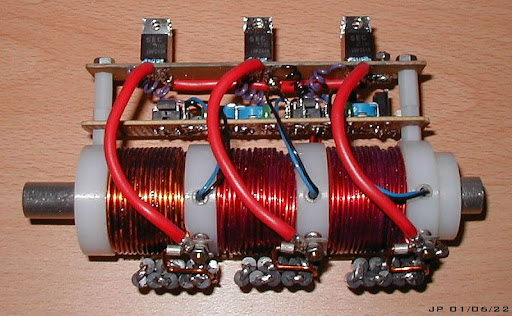
\includegraphics[width=7cm]{FigurasMemoria/fig1coilgunIntro.jpeg}
    \caption{Cañón de Gauss\citep{coilgun2024}.}
    \label{fig:prototipolanzadera} %Para referenciar -> \ref{fig:figNum}
\end{figure}

Las principales aplicaciones de las lanzaderas electromagnéticas se encuentran en el ámbito militar\citep{inproceedings}, donde se utilizan para el lanzamiento de proyectiles a alta velocidad sin la necesidad de explosivos químicos. Esta tecnología ofrece ventajas significativas, como la reducción del desgaste mecánico y la capacidad de ajustar la fuerza de lanzamiento con precisión. Además, en el sector aeroespacial\citep{inproceedings}, las lanzaderas electromagnéticas se consideran una alternativa prometedora para el lanzamiento de satélites y otros objetos al espacio, debido a su eficiencia energética y menor impacto ambiental en comparación con los cohetes tradicionales. También encontramos varias aplicaciones en la industria, como por ejemplo en procesos de manufactura que requieren la propulsión de materiales a altas velocidades. También se están explorando aplicaciones en el campo de la medicina, como en dispositivos de resonancia magnética y aceleradores de partículas para tratamientos médicos avanzados\citep{inproceedings}.

Para finalizar con la introducción, se presentará brevemente el funcionamiento básico de estos cañones. El objetivo físico de una lanzadera electromagnética es la creación de un campo magnético mediante el paso de una corriente eléctrica a través de una bobina de cobre. Cuando se aplica corriente a la bobina, se genera un campo magnético que ejerce una fuerza de atracción sobre el proyectil, que debe ser de material ferromagnético, al que me referiré durante este proyecto como \textbf{vástago}. El proceso de aceleración comienza cuando la corriente eléctrica, controlada por un circuito electrónico, fluye a través de la bobina, creando un campo magnético que atrae el proyectil hacia el centro de la bobina. Antes de que los centros de la bobina y el vástago estén alineados, la corriente se corta, provocando que este último continúe su movimiento hacia adelante debido a su inercia.

\newpage

\newpage
\section{Objetivos y motivación del proyecto}
\label{sec:motivacionyobjetivos}

\subsection{Objetivos y métodos}
Exploraremos ahora los principales objetivos del proyecto, desglosando cada parte constituyente y su resultado esperado. El principal propósito de este trabajo es el diseño de una práctica universitaria que se pueda realizar durante la asignatura de sistemas eléctricos, con la idea de atraer a nuevos ingenieros hacia el campo de la electricidad.

Para lograr este objetivo principal, el trabajo se dividirá en cuatro partes: desarrollo teórico, simulaciones, desarrollo de un prototipo y desarrollo de la práctica. Los objetivos y resultados esperados de cada parte son:

\begin{enumerate}
    \item \textbf{Desarrollo teórico:} Este apartado tiene como objetivo explorar las fórmulas que describen el comportamiento del vástago dentro de la bobina cuando es alimentada con corriente continua. El desarrollo resultará en una serie de fórmulas que constituirán un modelo del sistema, así como un programa que las implemente en una aplicación de \textit{MatLAB\textregistered}.
    \item \textbf{Simulaciones:} Las simulaciones tienen como objetivo obtener otro modelo teórico del sistema, utilizando el método de los elementos finitos a través del software \textit{ANSYS Maxwell\textregistered}. El resultado esperado es un modelo paramétrico que permita introducir los valores de la geometría de la bobina y su alimentación, y devuelva los valores dinámicos del vástago. Se espera que estos resultados sean más precisos que los obtenidos mediante el desarrollo teórico.
    \item \textbf{Prototipo:} Esta parte tiene como objetivo el diseño y desarrollo de un prototipo funcional de lanzadera que permita comparar los resultados teóricos con los físicos. Será necesario diseñar un circuito electrónico de control con \textit{Arduino\textregistered} y un medio físico para sujetar y alimentar la bobina. El resultado esperado es un prototipo manejable y modular, con el cual se puedan probar diferentes configuraciones.
    \item \textbf{Desarrollo de la práctica:} Con los resultados obtenidos en los apartados anteriores, se desarrollará un documento que presente el diseño de una bobina para implementar en el prototipo, a resolver por los alumnos que realicen la práctica. Se especificarán las variables que pueden modificar, así como las relaciones entre ellas, definidas a partir de las ecuaciones de electromagnetismo que gobiernan los circuitos magnéticos.
\end{enumerate}

\newpage
\subsection{Motivación}

El desarrollo de este proyecto está justificado por los siguientes puntos, que van a ser las principales áreas de influencia de este trabajo de final de grado:

\begin{enumerate}
    \item \textbf{Vanguardia Tecnológica:} La investigación y desarrollo en tecnologías como la tratada en este trabajo representan una oportunidad para estar a la vanguardia en el campo de la ingeniería electromagnética. Este proyecto permite explorar y comprender los principios fundamentales del electromagnetismo aplicados a un sistema real y funcional.
    \item \textbf{Aplicación de Conocimientos Teóricos:} La creación de una \textit{lanzadera electromagnética} requiere la aplicación de conocimientos avanzados en física, matemáticas e ingeniería eléctrica. Este proyecto proporciona un contexto práctico en el que tanto el autor como alumno, como los futuros estudiantes que lo utilicen, emplearán teorías y conceptos aprendidos en las aulas para fortalecer su entendimiento de los fenómenos electromagnéticos a un nivel visual y palpable.
    \item \textbf{Desarrollo de Competencias Técnicas:} La construcción de la \textit{lanzadera} involucra diversas habilidades técnicas, desde el diseño y simulación en software especializado hasta la fabricación y prueba de placas electrónicas y prototipos funcionales. Este proceso mejora significativamente las competencias prácticas en el laboratorio, una habilidad esencial para cualquier ingeniero eléctrico.
    \item \textbf{Fomento de la Innovación Educativa:} El desarrollo de este proyecto no solo busca aportar al conocimiento técnico, sino también servir como una herramienta educativa innovadora. La práctica universitaria diseñada a partir de este proyecto permitirá a los estudiantes experimentar directamente con la optimización de parámetros electromagnéticos, desarrollando habilidades críticas y fomentando una mentalidad innovadora.
\end{enumerate}

Con esto queda justificada la realización de este proyecto de fin de grado, y podemos empezar a desarrollar el proceso de creación de la \textbf{lanzadera electromagnética}.

\newpage
\input{MarcoTeorico.tex}

\newpage
\section{Cálculo analítico de la fuerza de atracción}
\label{sec:analitico}
En la sección de desarrollo teórico trataré de proporcionar un procedimiento mediante el cual los alumnos que realicen la práctica sean capaces de optimizar la velocidad y fuerza del proyectil a partir de los parámetros eléctricos y geométricos que definen el sistema. Estos parámetros de entrada serán:
\begin{itemize}
    \item \textbf{Parámetros geométricos}:
    \begin{enumerate}[label=\alph*., leftmargin=*, itemindent=1em]
        \item \(r_{cext}\) y \(r_{cint} \): radios exterior e interior de la bobina, respectivamente.
        \item \(l_c\): altura de la bobina.
        \item \(r_{fe}\): radio del vástago.
        \item \(l_{fe}\): longitud del vástago.
        \item \(k_{disp}\): parámetro multiplicador para obtener la sección de dispersión. La dispersión es la parte del flujo que abraza a la bobina y a la barra.
    \end{enumerate}
    \item \textbf{Parámetros eléctricos}:
    \begin{enumerate}[label=\alph*., leftmargin=*, itemindent=1em]
        \item \(N\): número de espiras.
        \item \(I_{cc}\): corriente de alimentación del solenoide.
        \item \(\mu_{fe}\): permeabilidad relativa del vástago ferromagnético.
    \end{enumerate}
\end{itemize}

\begin{figure}[H]
    \centering 
    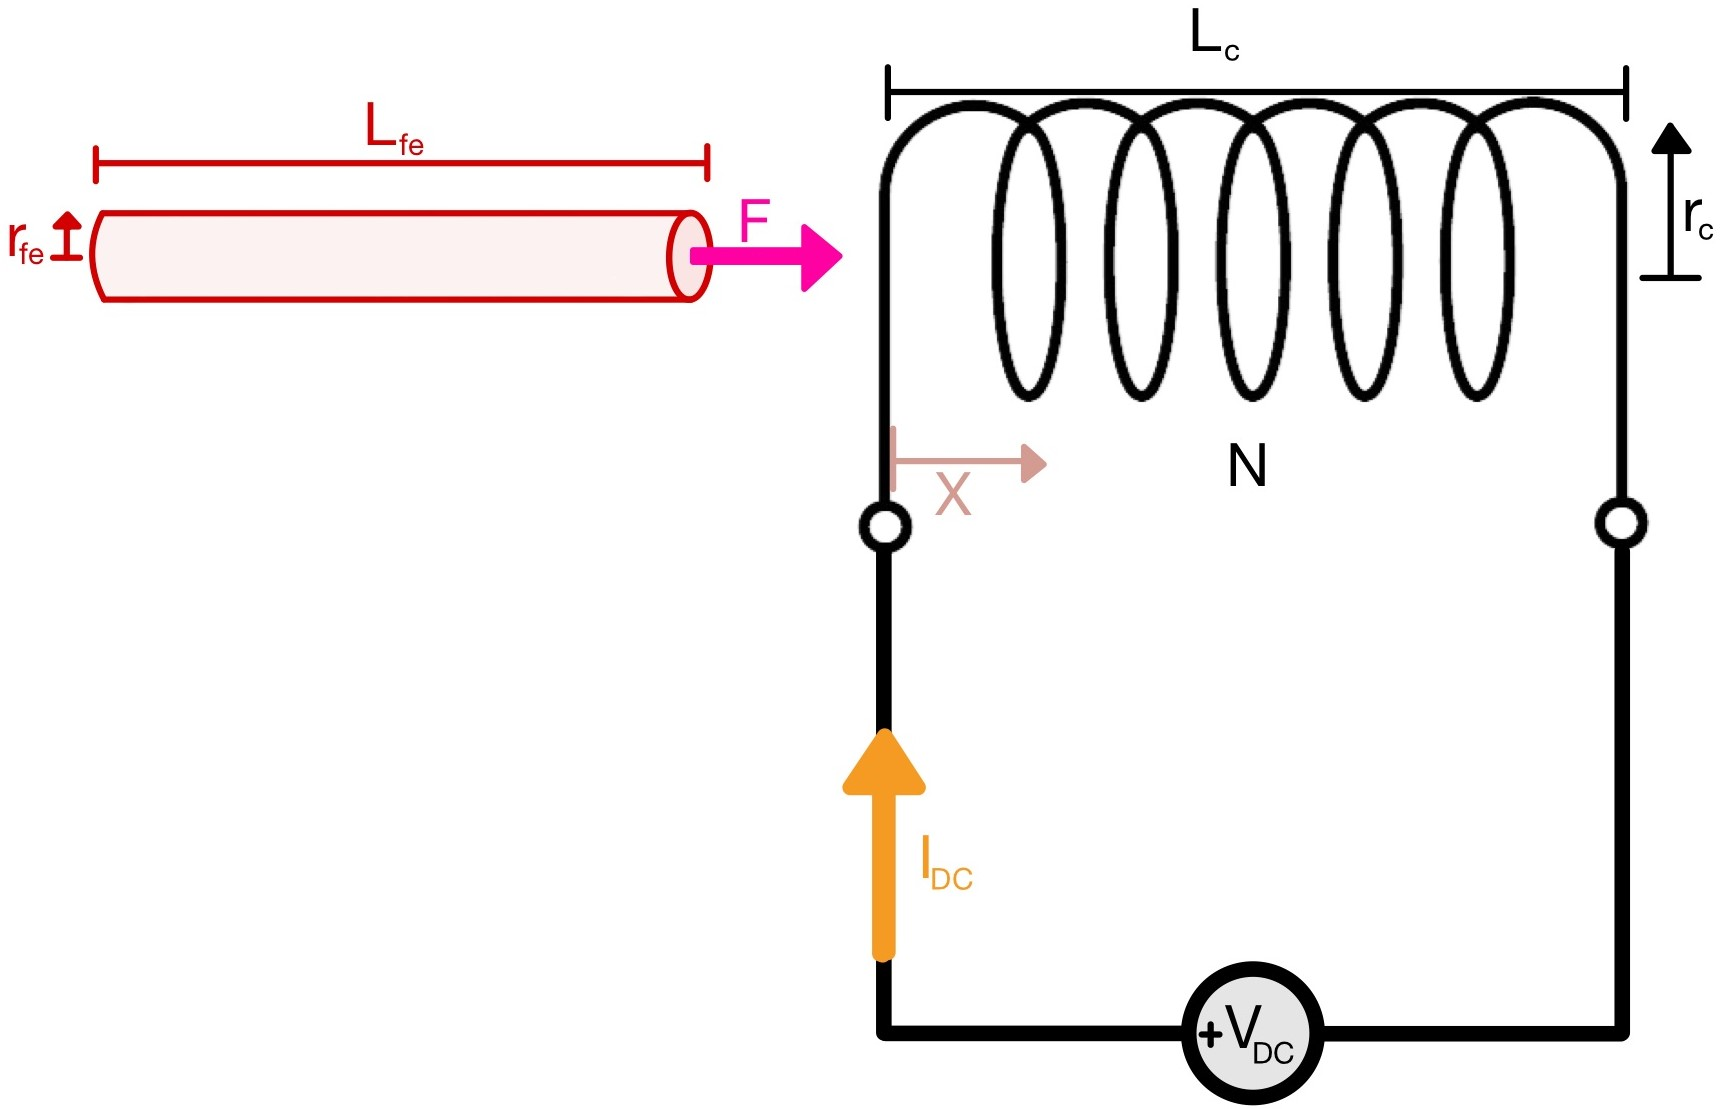
\includegraphics[width=10cm]{FigurasMemoria/esquemaDesTeor.jpg}
    \caption{Esquema geométrico del sistema. Elaboración propia.}
    \label{fig:esquemaDesTeor} %Para referenciar -> \ref{fig:figNum}
\end{figure}

El objetivo de este desarrollo es crear un programa en MATLAB al que se le proporcionen estos datos, y con ellos calcule automáticamente la fuerza que experimentará el proyectil a través del circuito magnético del sistema. Como se muestra en la figura \ref{fig:electromagnet} el valor de \(B\) varía a lo largo del solenoide, por lo tanto, además de los parámetros constantes dados, será necesario parametrizar también la posición del vástago en cada momento (\(x\) en la figura \ref{fig:esquemaDesTeor}) y calcular la fuerza que experimenta en cada una de esas posiciones.

El primer paso será partir de las fórmulas del circuito magnético definidas en el \ref{sec:marcoteorico} marco teórico y para ello la primera tarea es realizar un análisis de las diferentes reluctancias del sistema, con el objetivo de computar así la inducción magnética, la cual nos permitirá obtener la fuerza de atracción que experimenta el vástago, que según Nicolás Jerez \citep{jerez2016resueltos} viene dada por la expresión:

\begin{center}
\[F=\frac{1}{2}\frac{B^2*S}{\mu_0}\]
\end{center}

Teniendo clara la relación entre inducción y fuerza, el siguiente paso es definir claramente las diferentes áreas efectivas de los componentes del sistema para calcular las reluctancias, las cuales son:

\begin{itemize}
    \item \(S_{c}=\pi *r_{cext}^2\): Esta superficie se corresponde con la sección delimitada por el radio exterior de la bobina, y es el área efectiva del flujo encerrado en su interior.
    \item \(S_{fe}=\pi *r_{fe}^2\): Esta superficie se corresponde con la sección delimitada por el radio del vástago.
    \item \(S_{disp}=\pi *r_{disp}~~\forall r_{disp} = k_{disp}r_c\): Esta superficie se corresponde con el área de dispersión de flujo.
\end{itemize}

\begin{figure}[H]
    \centering
    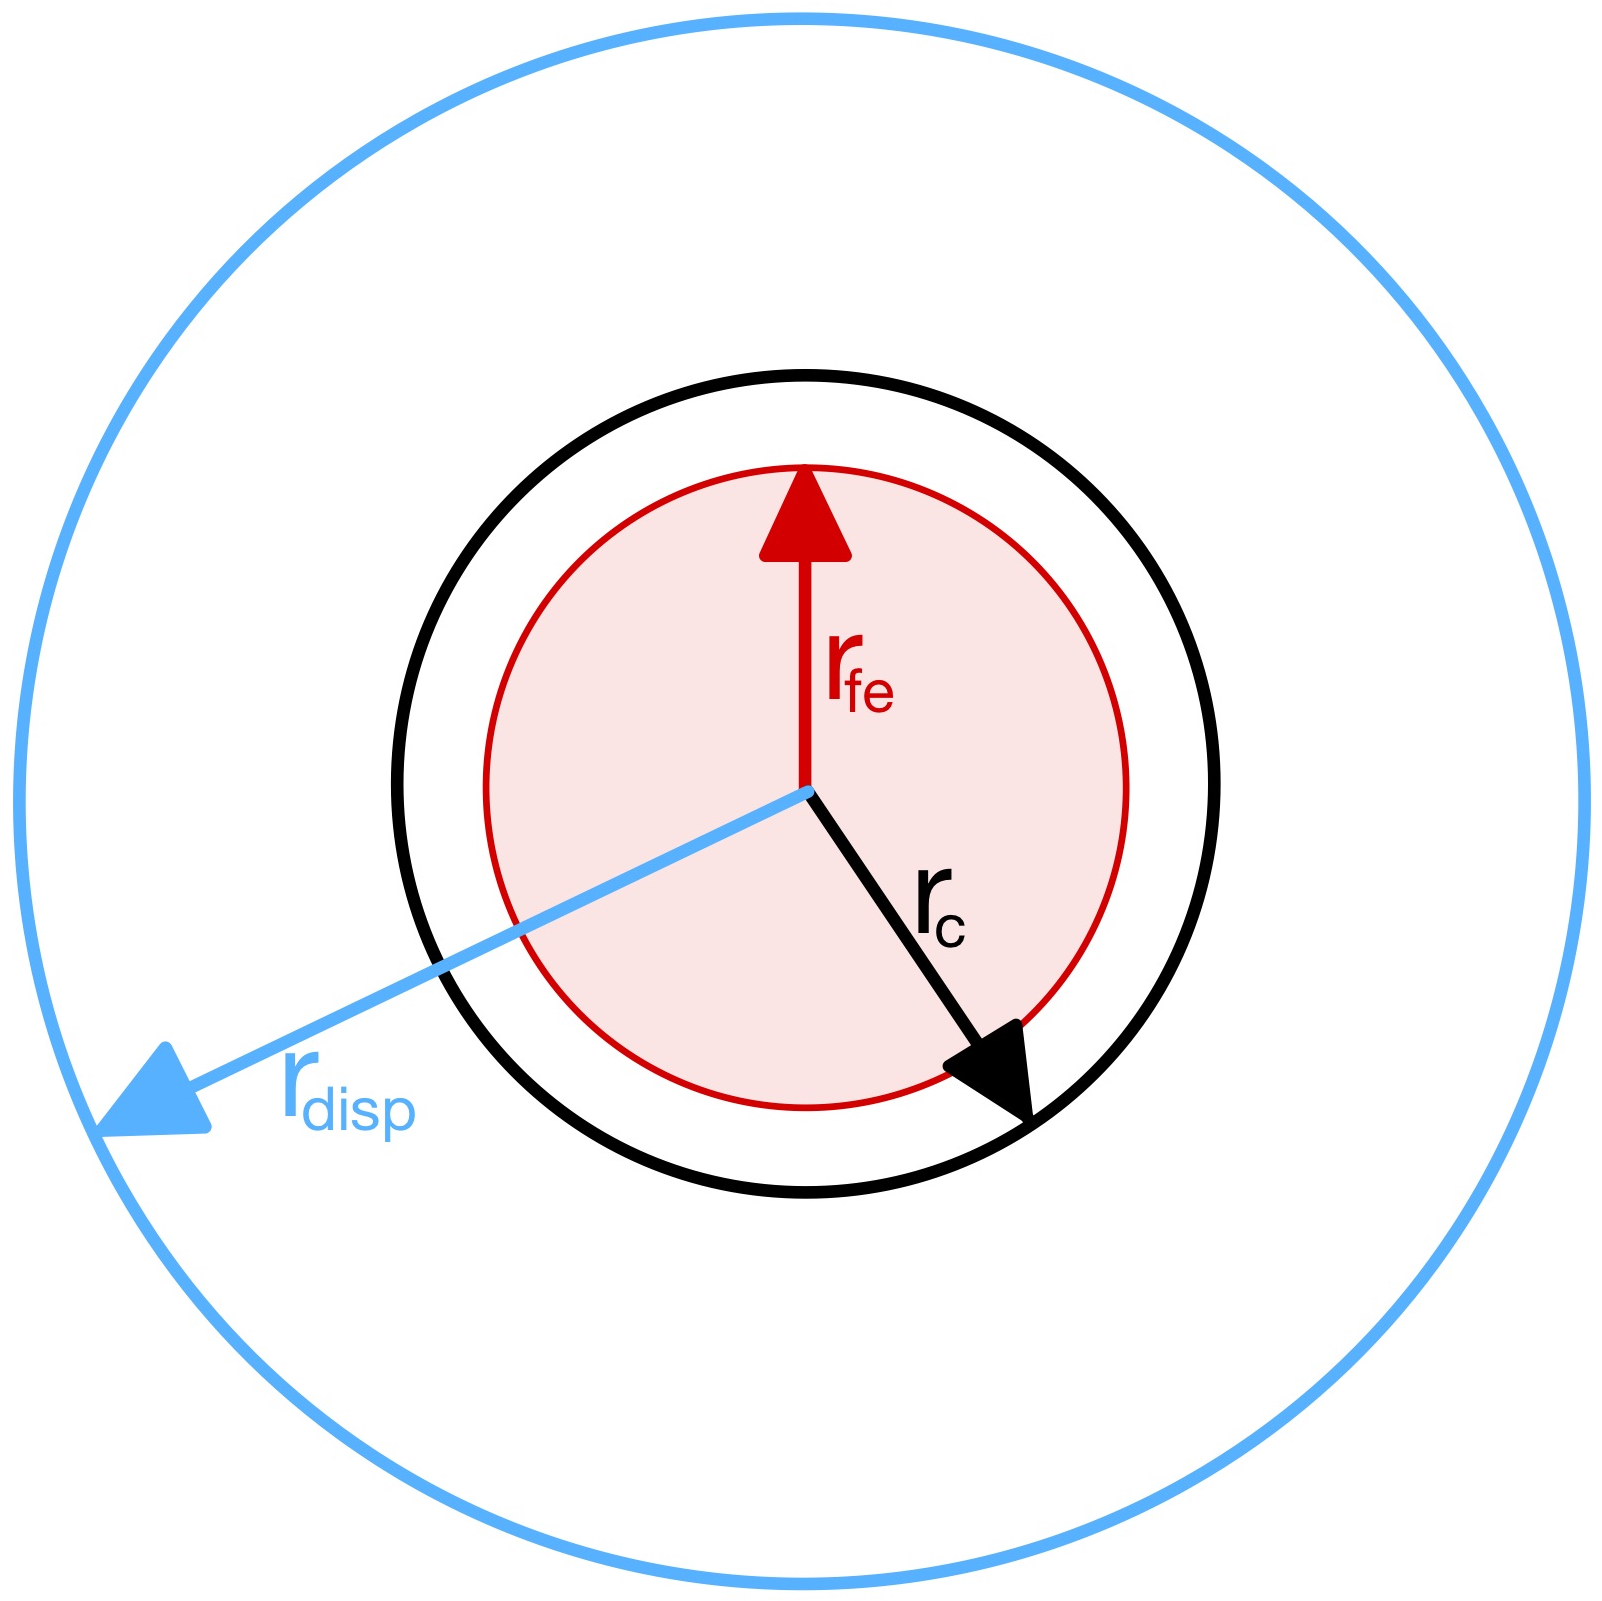
\includegraphics[width=5cm]{FigurasMemoria/areasFlujo.jpg}
    \caption{Secciones del sistema con una vista de planta. Elaboración propia.}
    \label{fig:areasFlujo} %Para referenciar -> \ref{fig:figNum}
\end{figure}

Teniendo en cuenta las fórmulas en la sección del marco teórico (\ref{sec:marcoteorico}) y lo expuesto en la figura \ref{fig:areasFlujo}, podemos concluir que existen cuatro principales reluctancias en el sistema de la figura \ref{fig:esquemaDesTeor}:

\begin{itemize}
    \item \(\mathcal{R}_{disp~c}=\frac{h_c}{\mu_0*S_{disp}}\): Se corresponde a la reluctancia del aire que abraza la bobina. Esta reluctancia es fija ya que las dimensiones del solenoide son constantes.
    \item \(\mathcal{R}_{fe}=\frac{l_{fe}}{\mu_0*\mu_{fe}*S_{fe}}\): Se corresponde a la reluctancia de la barra. Esta reluctancia es fija ya que las dimensiones del vástago son constantes.
    \item \(\mathcal{R}_{\phi}=\frac{(h_c+l_{fe})-x}{\mu_0*S_{disp}}\): Se corresponde a la reluctancia del aire del camino más largo del flujo magnético, y es la que provoca que el campo del electroimán interactúe con el vástago. Es variable ya que la posición del vástago es variable y el camino se reduce con el tiempo.
    \item \(\mathcal{R}_{aire~c}=\frac{h_c-x}{\mu_0*S_c}\): Se corresponde a la reluctancia del aire en el interior de la bobina. Es variable ya que la cantidad de aire disminuye con la posición del vástago.
\end{itemize}

\begin{figure}[H]
    \centering
    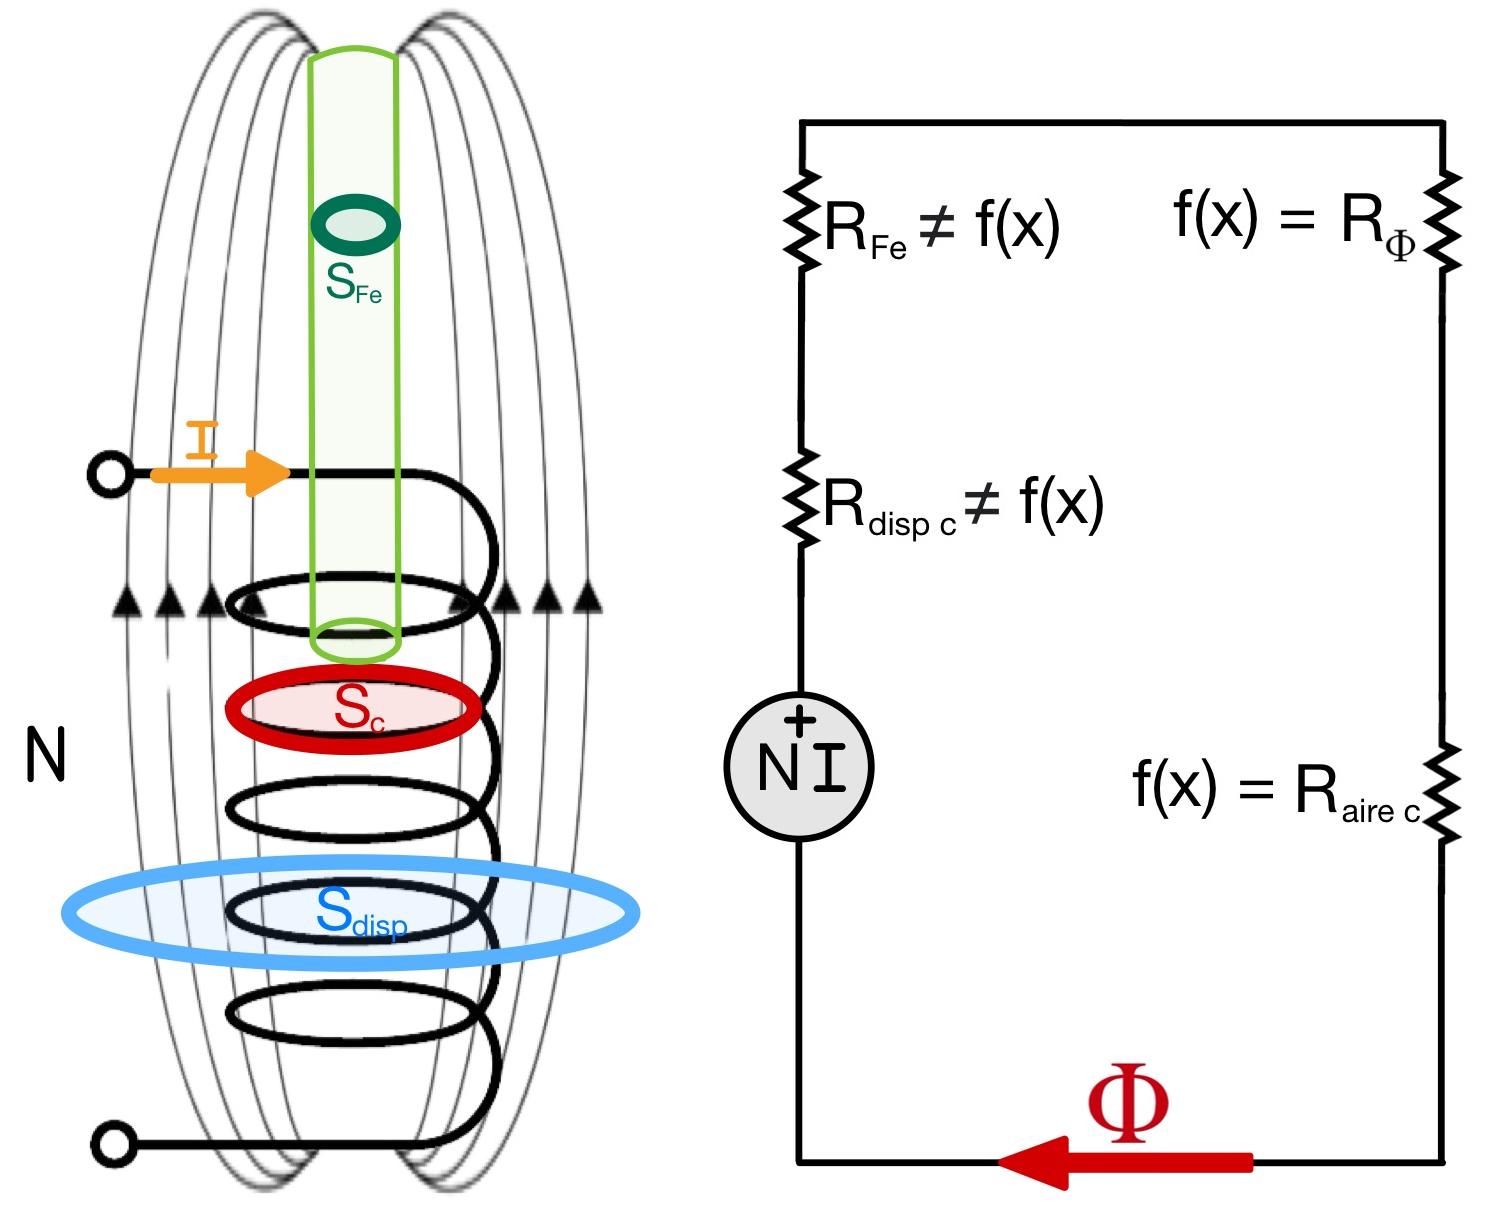
\includegraphics[width=11cm]{FigurasMemoria/circuitoMag.jpg}
    \caption{Circuito magnético del sistema.}
    \label{fig:circuitoMag} %Para referenciar -> \ref{fig:figNum}
\end{figure}


Con el circuito magnético definido, el siguiente paso es programar las relaciones presentadas en esta sección en MATLAB y graficar los resultados en función de la posición. El programa en MATLAB constará de tres secciones: definición, cálculos y graficación. El código se puede encontrar en el anexo 1 \ref{sec:anexo1}. El producto de este código es una ''calculadora'' que devuelve la evolución de la fuerza con el parámetro \(x\), y queda así:

\begin{figure}[H]
    \centering
    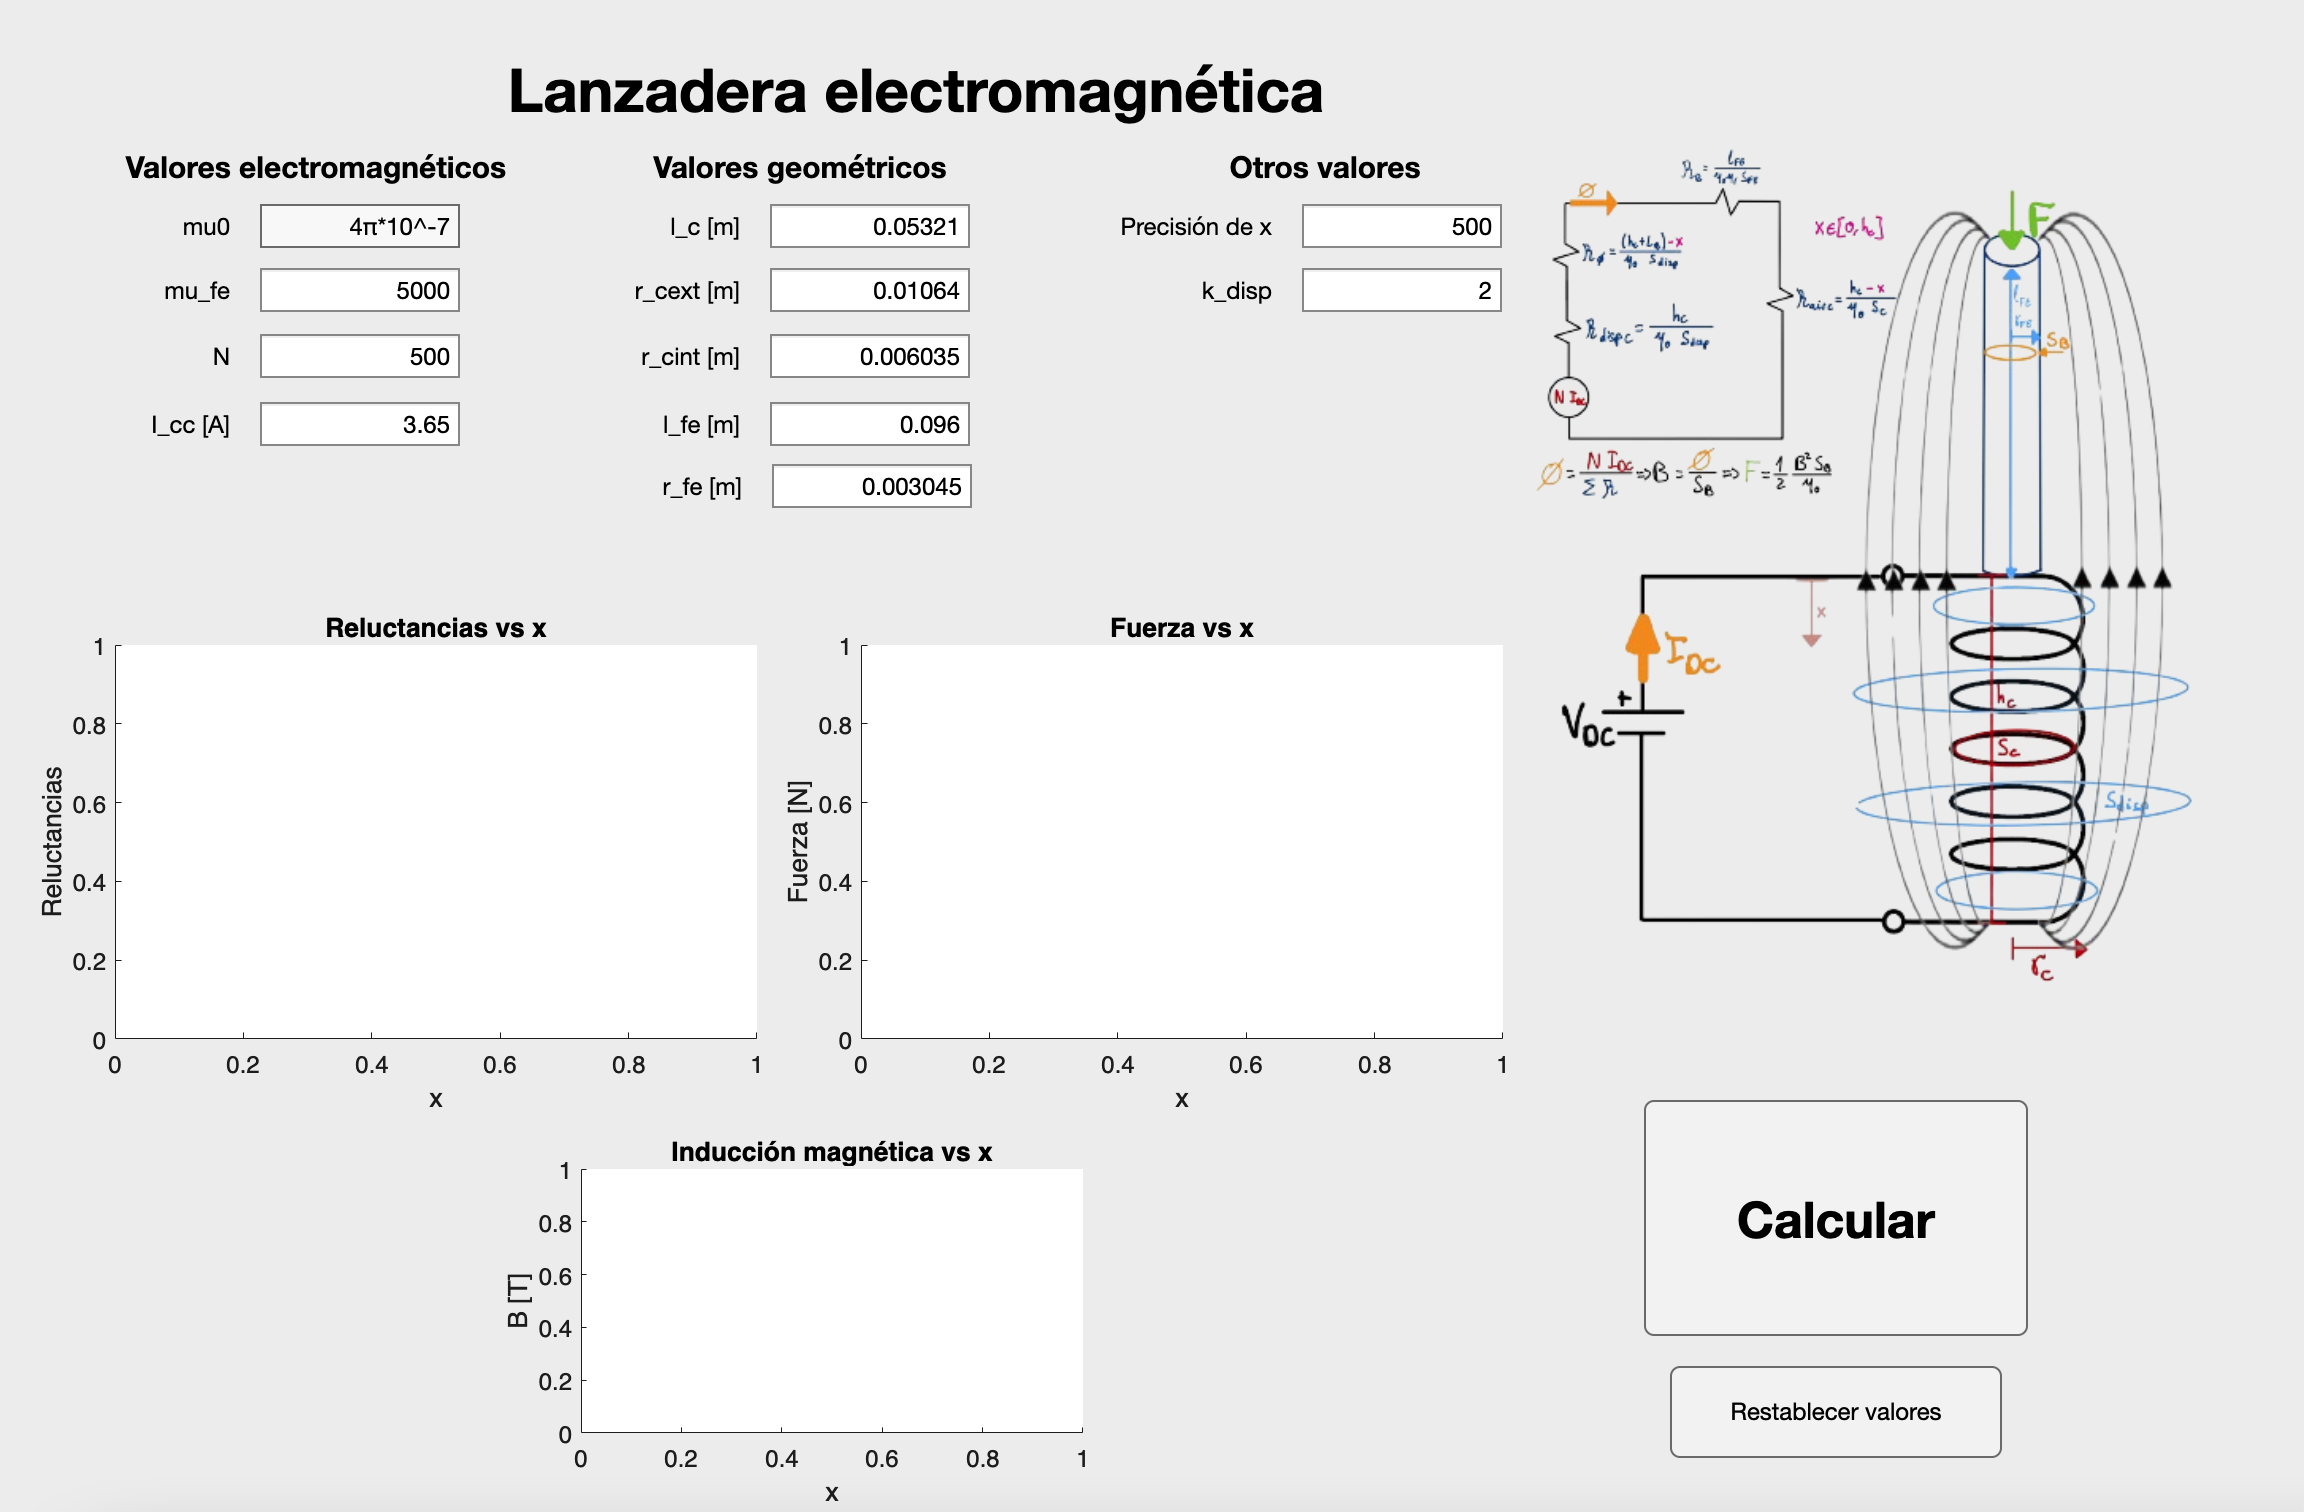
\includegraphics[width=13cm]{FigurasMemoria/calculadora.png}
    \caption{Aplicación de cálculos de MATLAB.}
    \label{fig:calculadora} %Para referenciar -> \ref{fig:figNum}
\end{figure}

Los valores escritos en las variables del sistema que se pueden ver en la figura \ref{fig:calculadora} se correponden con la bobina de ejemplo que se ha utilizado para crear el proyecto. Dicha bobina tiene la siguiente geometría:

\[
\begin{array}{c}
    \mu_0 = 4\pi \times 10^{-7}~~~~~~\mu_{fe} = 5000~~~~~~N = 500 \\
    l_{fe} = 0.096m~~~~~~r_{fe} = 0.003045m \\
    h_c = 0.05321m~~~~~~r_{c} = 0.01064m~~~~~~r_{disp} = k_{disp}~r_{c}=2~r_{c}
\end{array}
\]

Con esta configuración, la forma de las gráficas obtenidas es:

\begin{figure}[H]
    \centering
    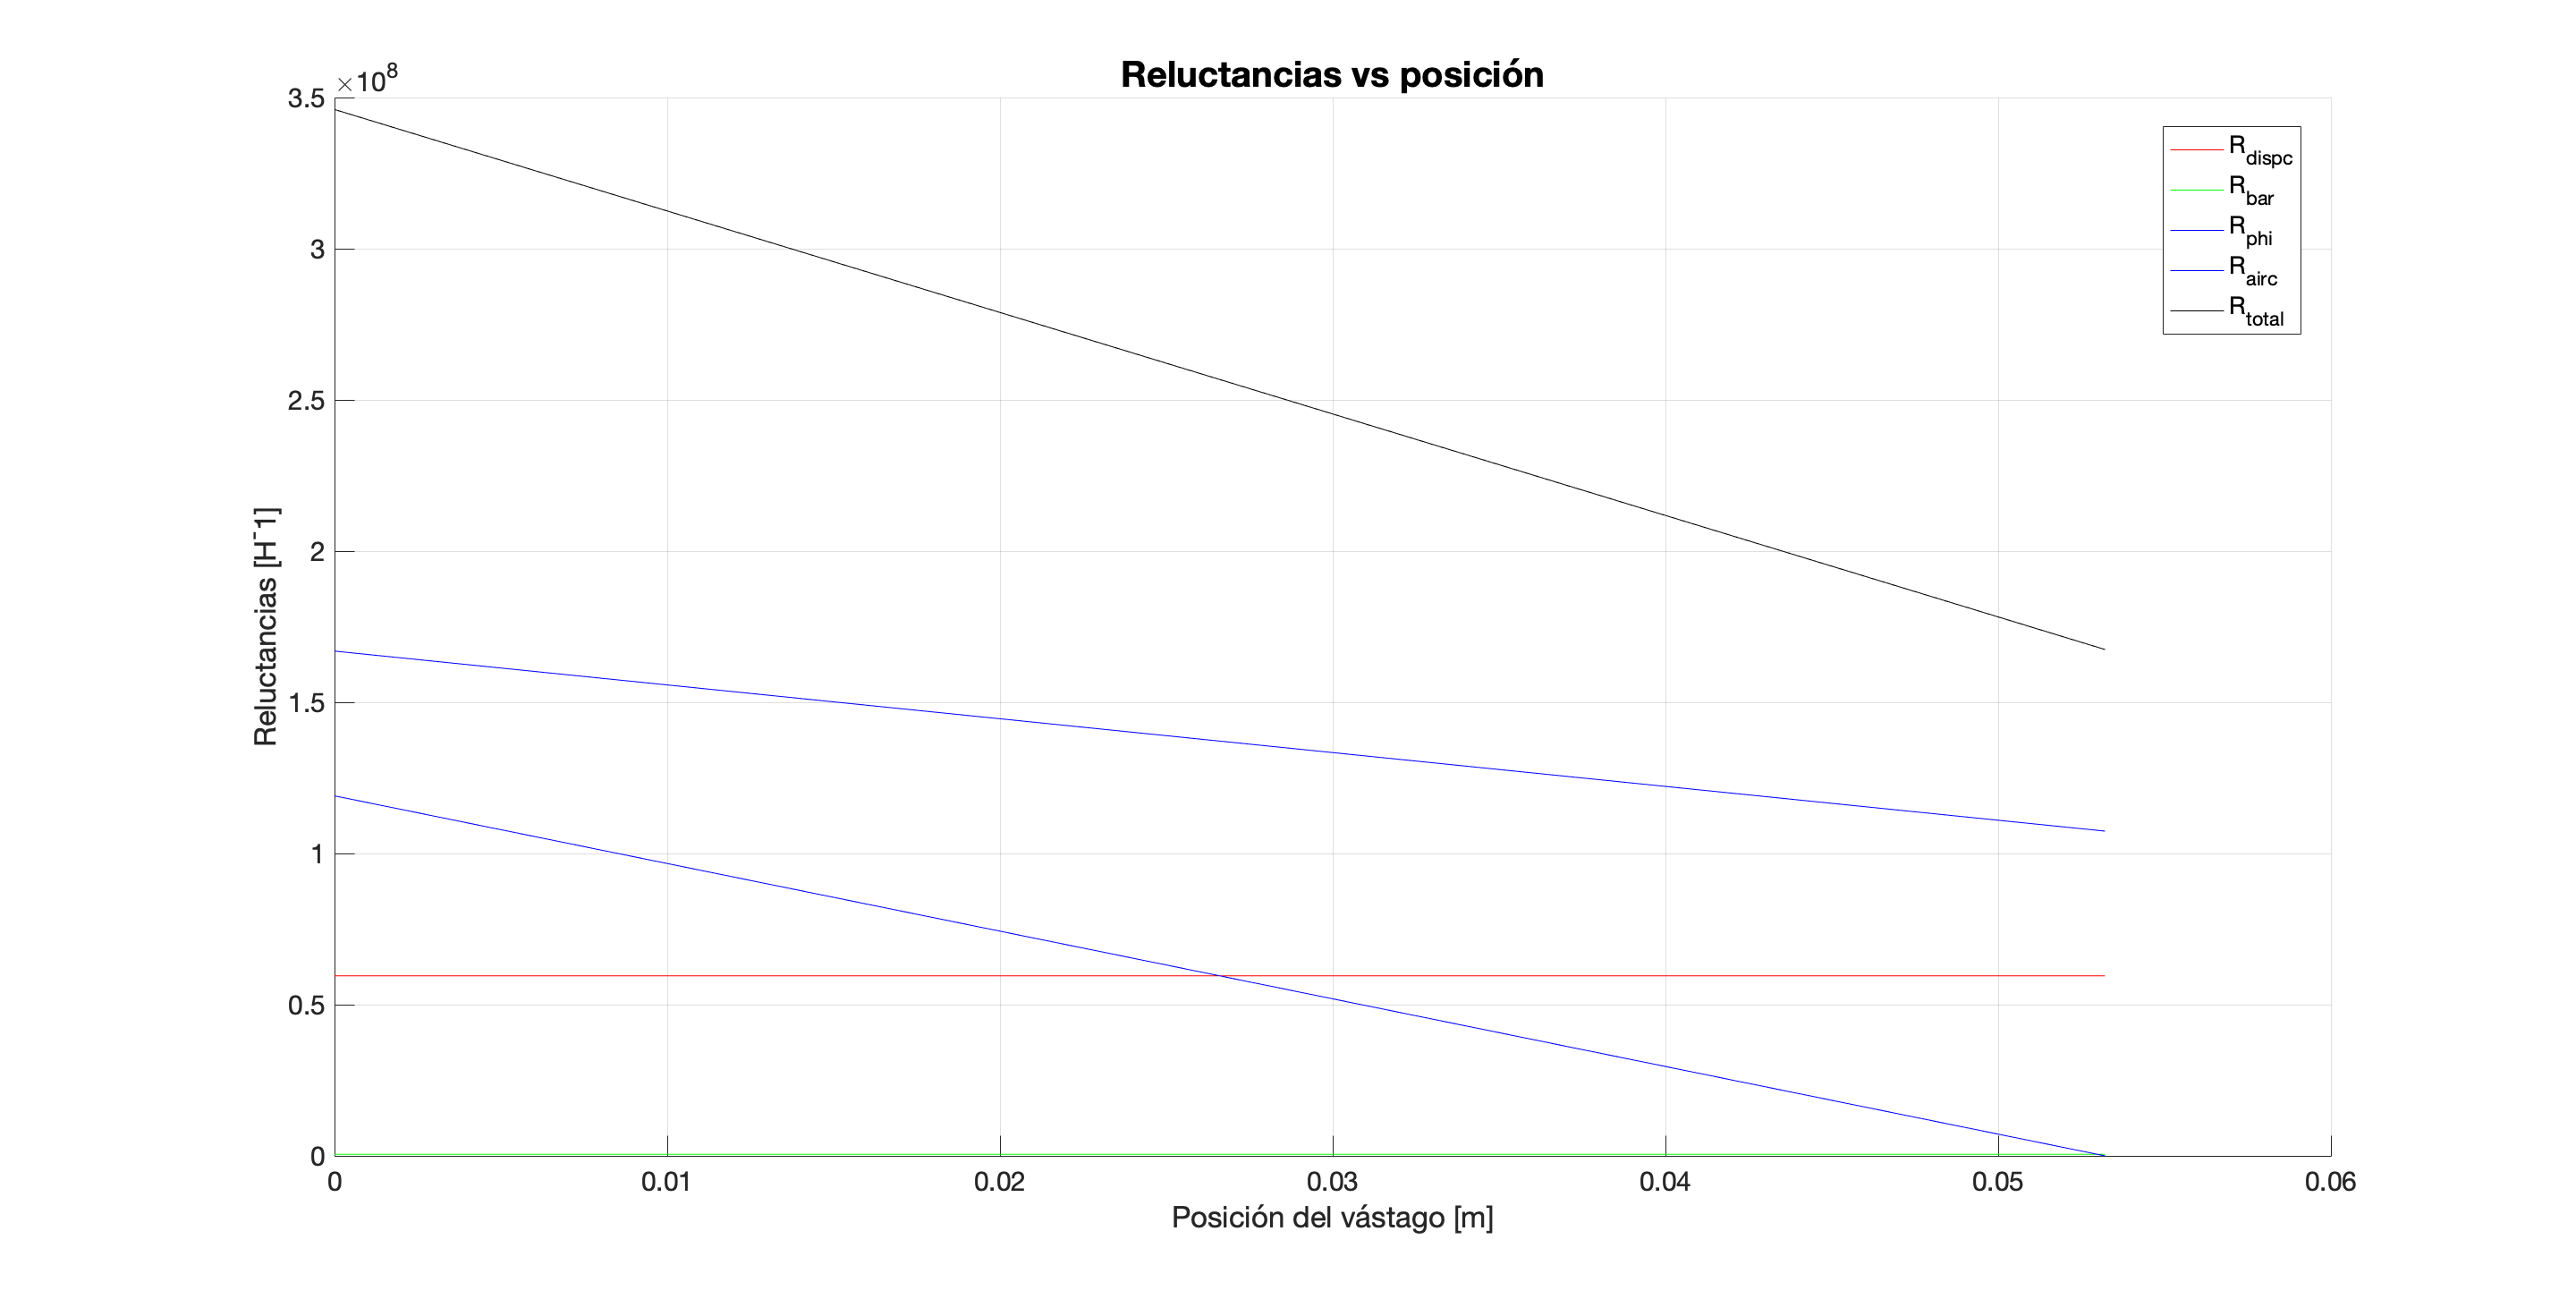
\includegraphics[width=13cm]{FigurasMemoria/calcRsetupBase.png}
    \caption{Reluctancias en función de la posición del vástago respecto a la bobina.}
    \label{fig:calcRsetupBase} %Para referenciar -> \ref{fig:figNum}
\end{figure}

\begin{figure}[H]
    \centering
    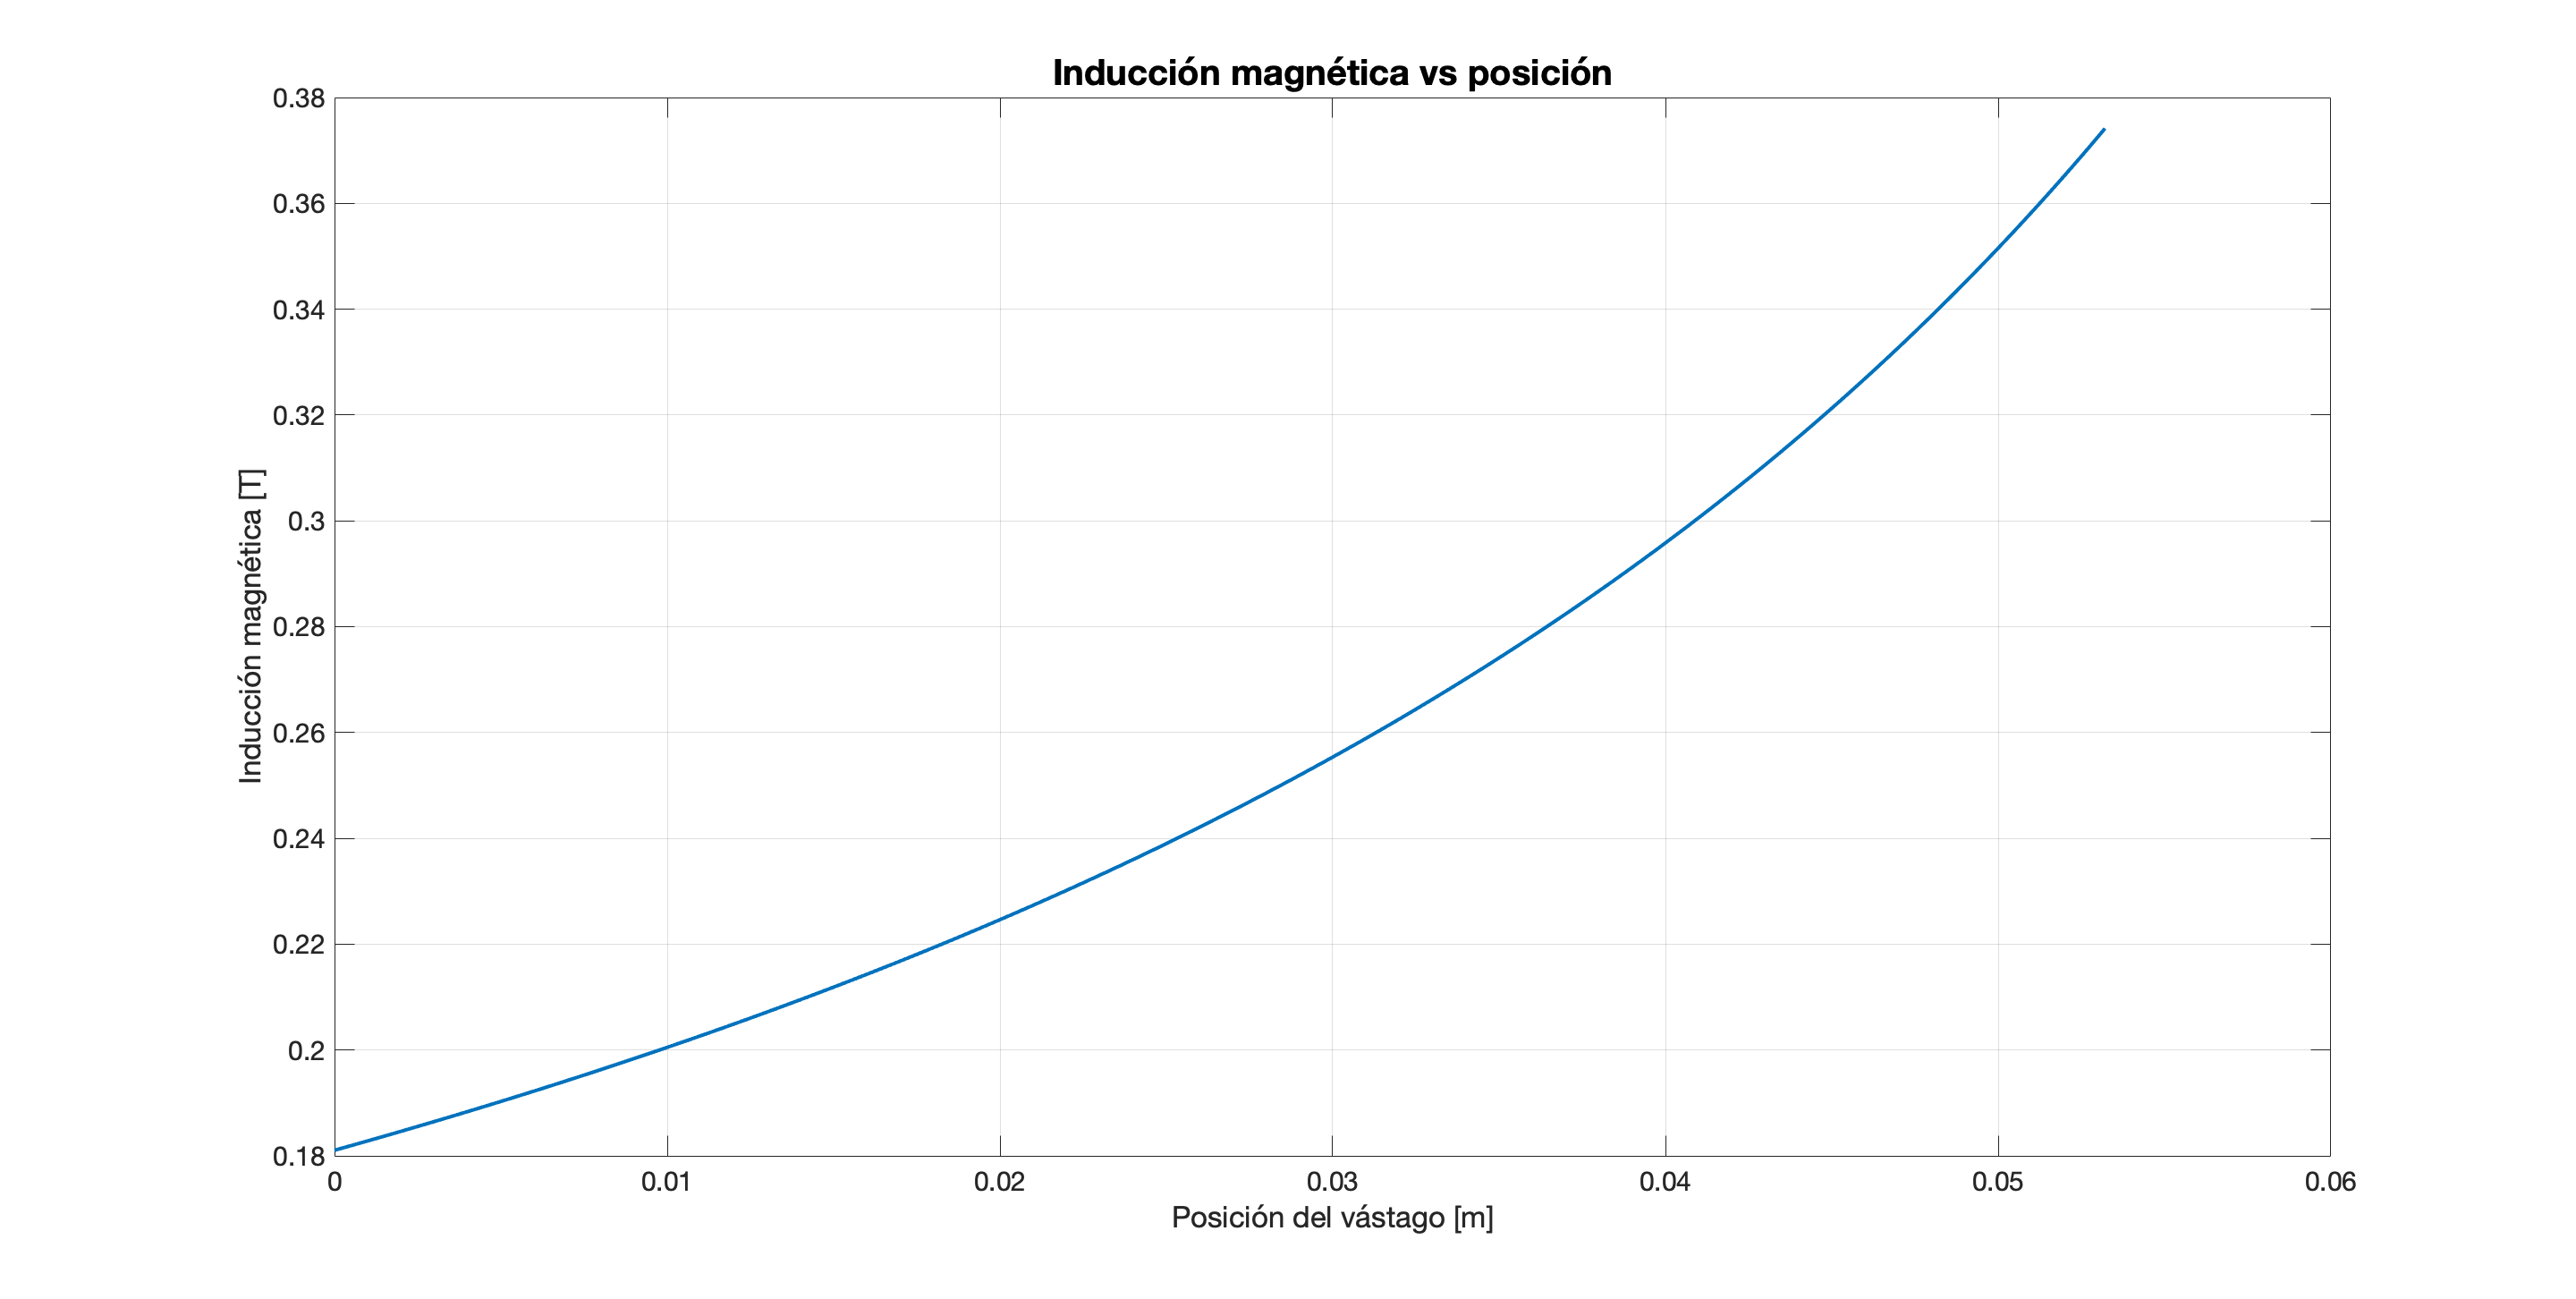
\includegraphics[width=\linewidth]{FigurasMemoria/calcBsetupBase.png}
    \caption{Inducción en función de la posición del vástago respecto a la bobina.}
    \label{fig:calcBsetupBase} %Para referenciar -> \ref{fig:figNum}
\end{figure}

\begin{figure}[H]
    \centering
    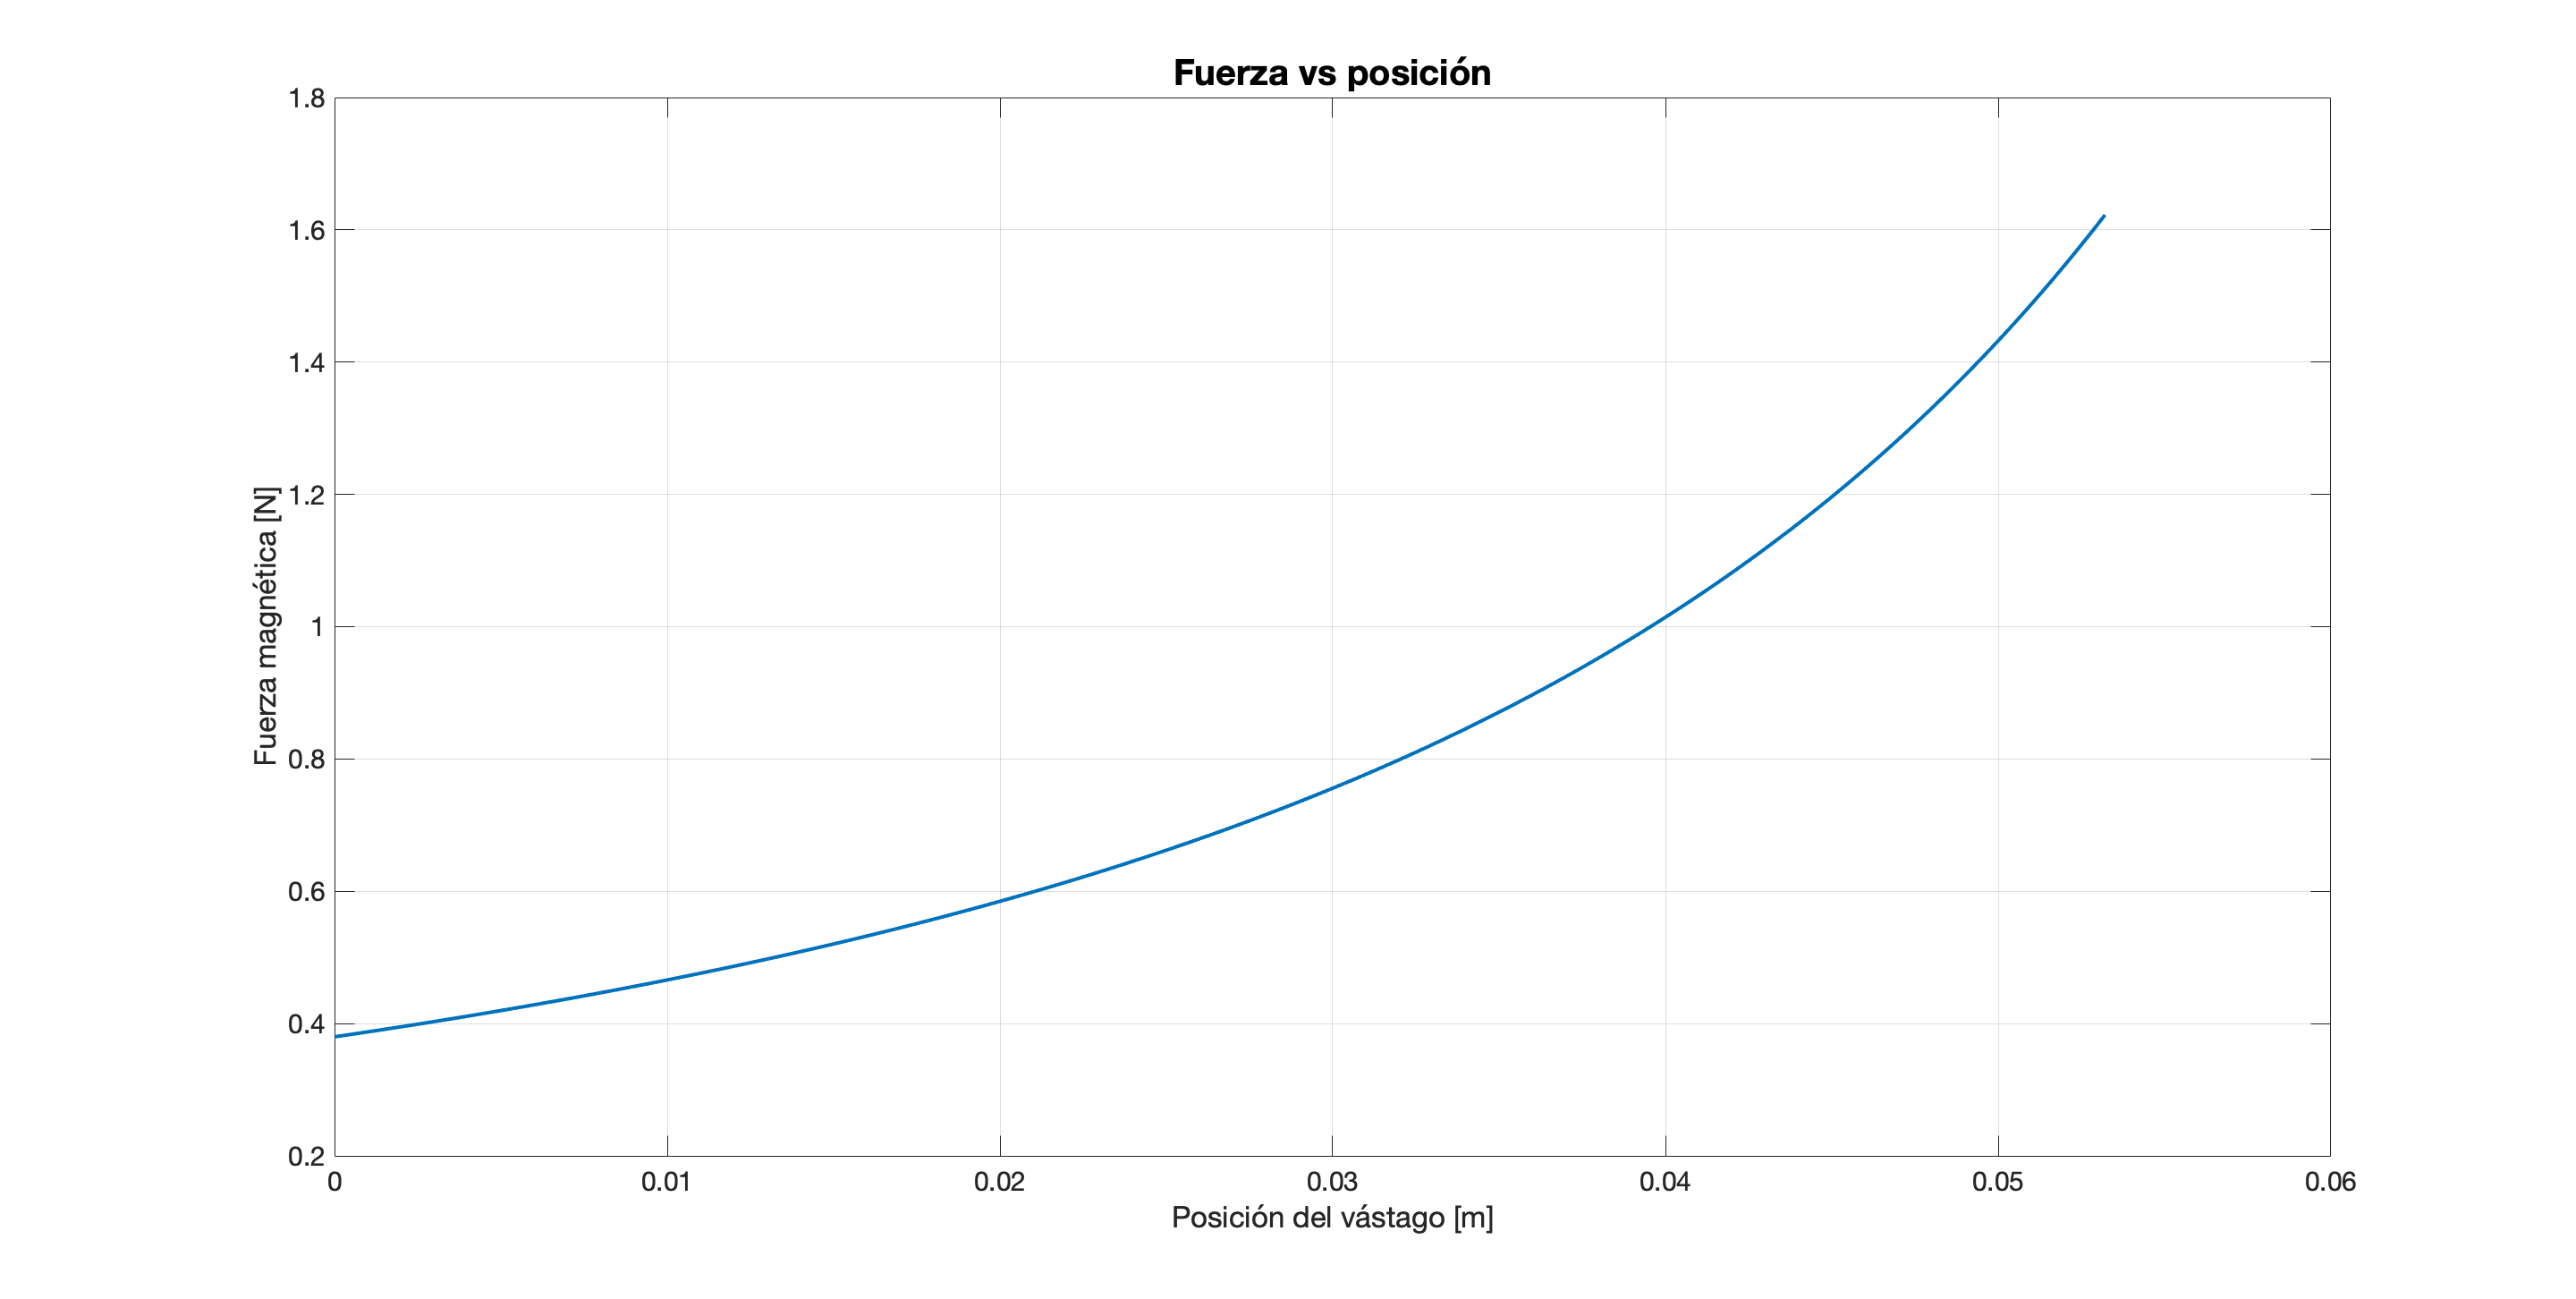
\includegraphics[width=\linewidth]{FigurasMemoria/calcFsetupBase.png}
    \caption{Fuerza en función de la posición del vástago respecto a la bobina.}
    \label{fig:calcFsetupBase} %Para referenciar -> \ref{fig:figNum}
\end{figure}

Estas figuras serán discutidas en el apartado de análisis de resultados \ref{sec:resultados}.

\noindent \textbf{Prueba inicial}
\\~\\
\indent Antes de continuar con el desarrollo, se ha realizado una prueba con un dinamómetro sobre la bobina de prueba especificada anteriormente, para verificar los resultados de la figura \ref{fig:calcFsetupBase} y poder continuar con las simulaciones y prototipo con una referencia. Se ha obtenido el siguiente resultado:

\begin{figure}[H]
    \centering
    
\includegraphics[width=9cm]{FigurasMemoria/dinamometro.jpeg}
    \caption{Dato experimental de fuerza con la bobina alimentada.}
    \label{fig:dinamometro} %Para referenciar -> \ref{fig:figNum}
\end{figure}

\[F_{barra}=2.4~N~\forall I_{cc}=3.5~A\]

\newpage
\input{Simulaciones.tex}

\newpage
\section{Desarrollo de un prototipo de lanzadera electromagnética}
\label{sec:prototipo}

El desarrollo del prototipo de la lanzadera electromagnética constituye una etapa crucial en la validación del modelo teórico y las diferentes simulaciones realizadas en fases previas. Esta sección se centra en el diseño y construcción de un dispositivo funcional que permita la evaluación práctica de los conceptos estudiados y la obtención de datos experimentales que respalden las predicciones teóricas.

El objetivo principal del prototipo es proporcionar una plataforma experimental (a la que se le llamará \textit{banco de pruebas}) que permita comprobar la efectividad de las configuraciones propuestas y realizar ajustes basados en observaciones empíricas. No se pretende construir una lanzadera electromagnética como la de la figura \ref{fig:prototipolanzadera}, sino más bien un prototipo modular que sea fácilmente modificable para poder probar diferentes configuraciones de bobina y alimentación. Una de las partes más importantes del prototipo ha sido la implementación de un sistema de medición capaz de registrar con exactitud la velocidad y fuerza del proyectil.

El siguiente apartado detalla los pasos específicos seguidos en el desarrollo del prototipo, desde el montaje del banco de pruebas, el diseño del circuito electrónico y la construcción de la bobina, hasta el ensamblaje sistema completo, así como algunas de las consideraciones de diseño que los alumnos tendrán que tener en cuenta a la hora de realizar la práctica.

\begin{figure}[H]
    \centering
    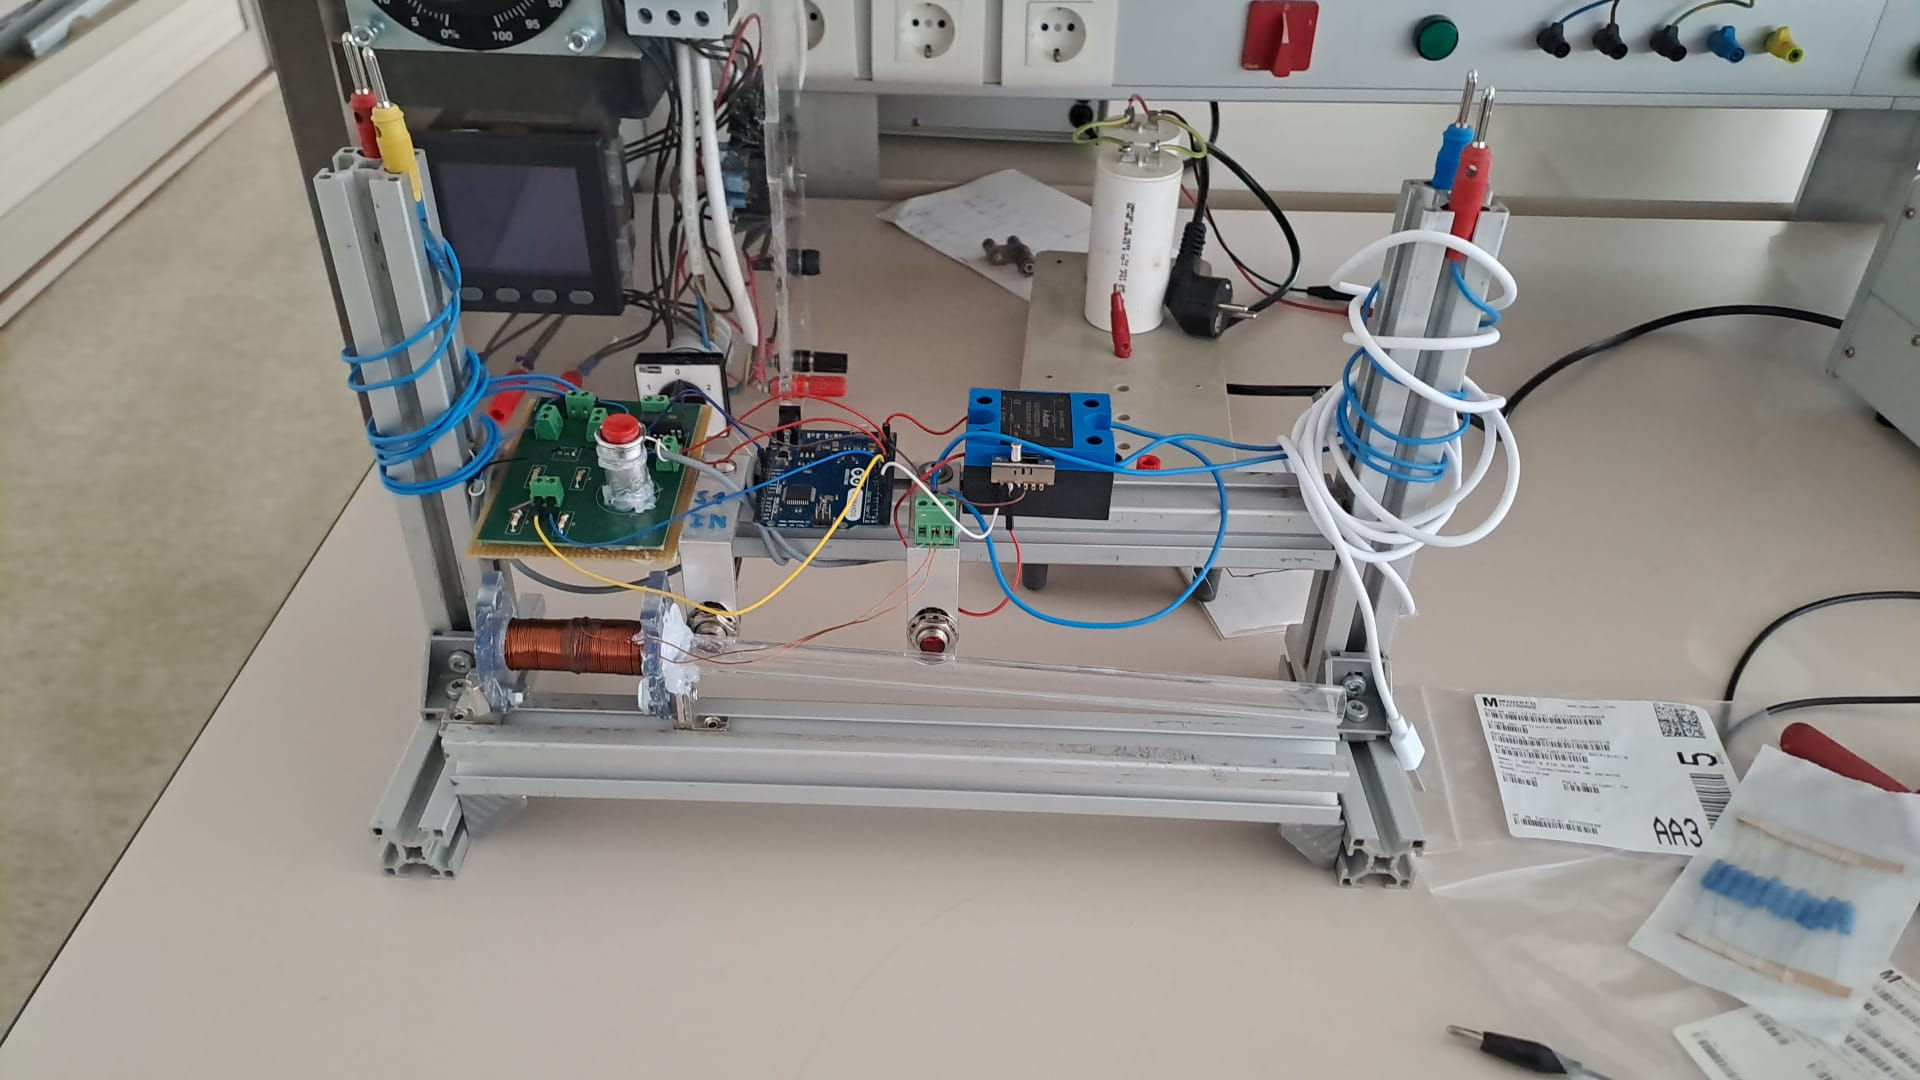
\includegraphics[width=\textwidth]{FigurasMemoria/prototipoFinal.jpg}
    \caption{Imagen del banco de pruebas definitivo.}
    \label{fig:prototipoFinal} %Para referenciar -> \ref{fig:figNum}
\end{figure}

\newpage

\subsection{Prueba inicial}

Antes de continuar con el desarrollo del prototipo, se ha realizado una prueba con un dinamómetro sobre la bobina de prueba especificada anteriormente para poder validar los resultados obtenidos en los apartados anteriores respecto a una referencia. El resultado obtenido es el siguiente:

\begin{figure}[H]
    \centering
    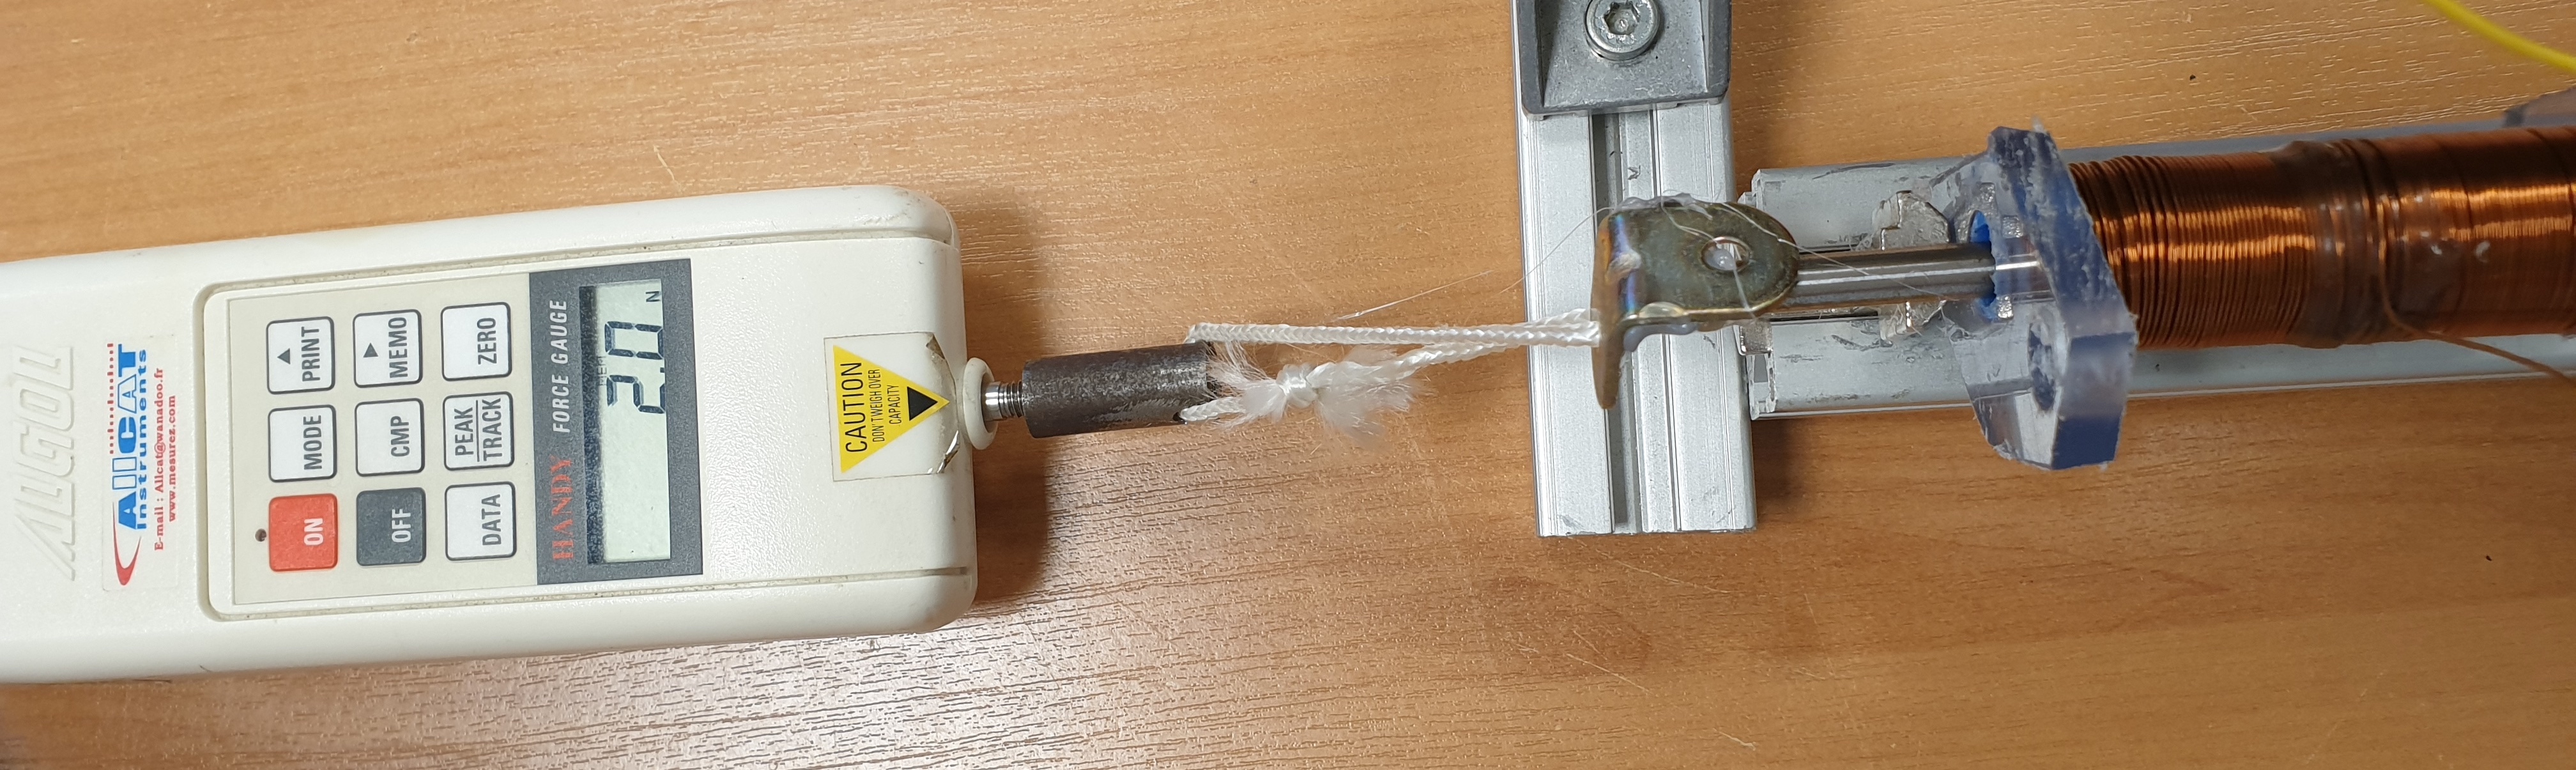
\includegraphics[width=9cm]{FigurasMemoria/dinamometro.jpg}
    \caption{Dato experimental de fuerza con la bobina alimentada.}
    \label{fig:dinamometro} %Para referenciar -> \ref{fig:figNum}
\end{figure}

\[F_{barra}=2~\text{N}~\forall I_{cc}=3.5~\text{A}\]

\subsection{Estructura}
\label{subsec:estructura}
Para construir una estructura estable para el banco de pruebas, se utilizaron perfiles técnicos estructurales de aluminio como el que se presenta en la siguiente figura:

\begin{figure}[H]
    \centering
    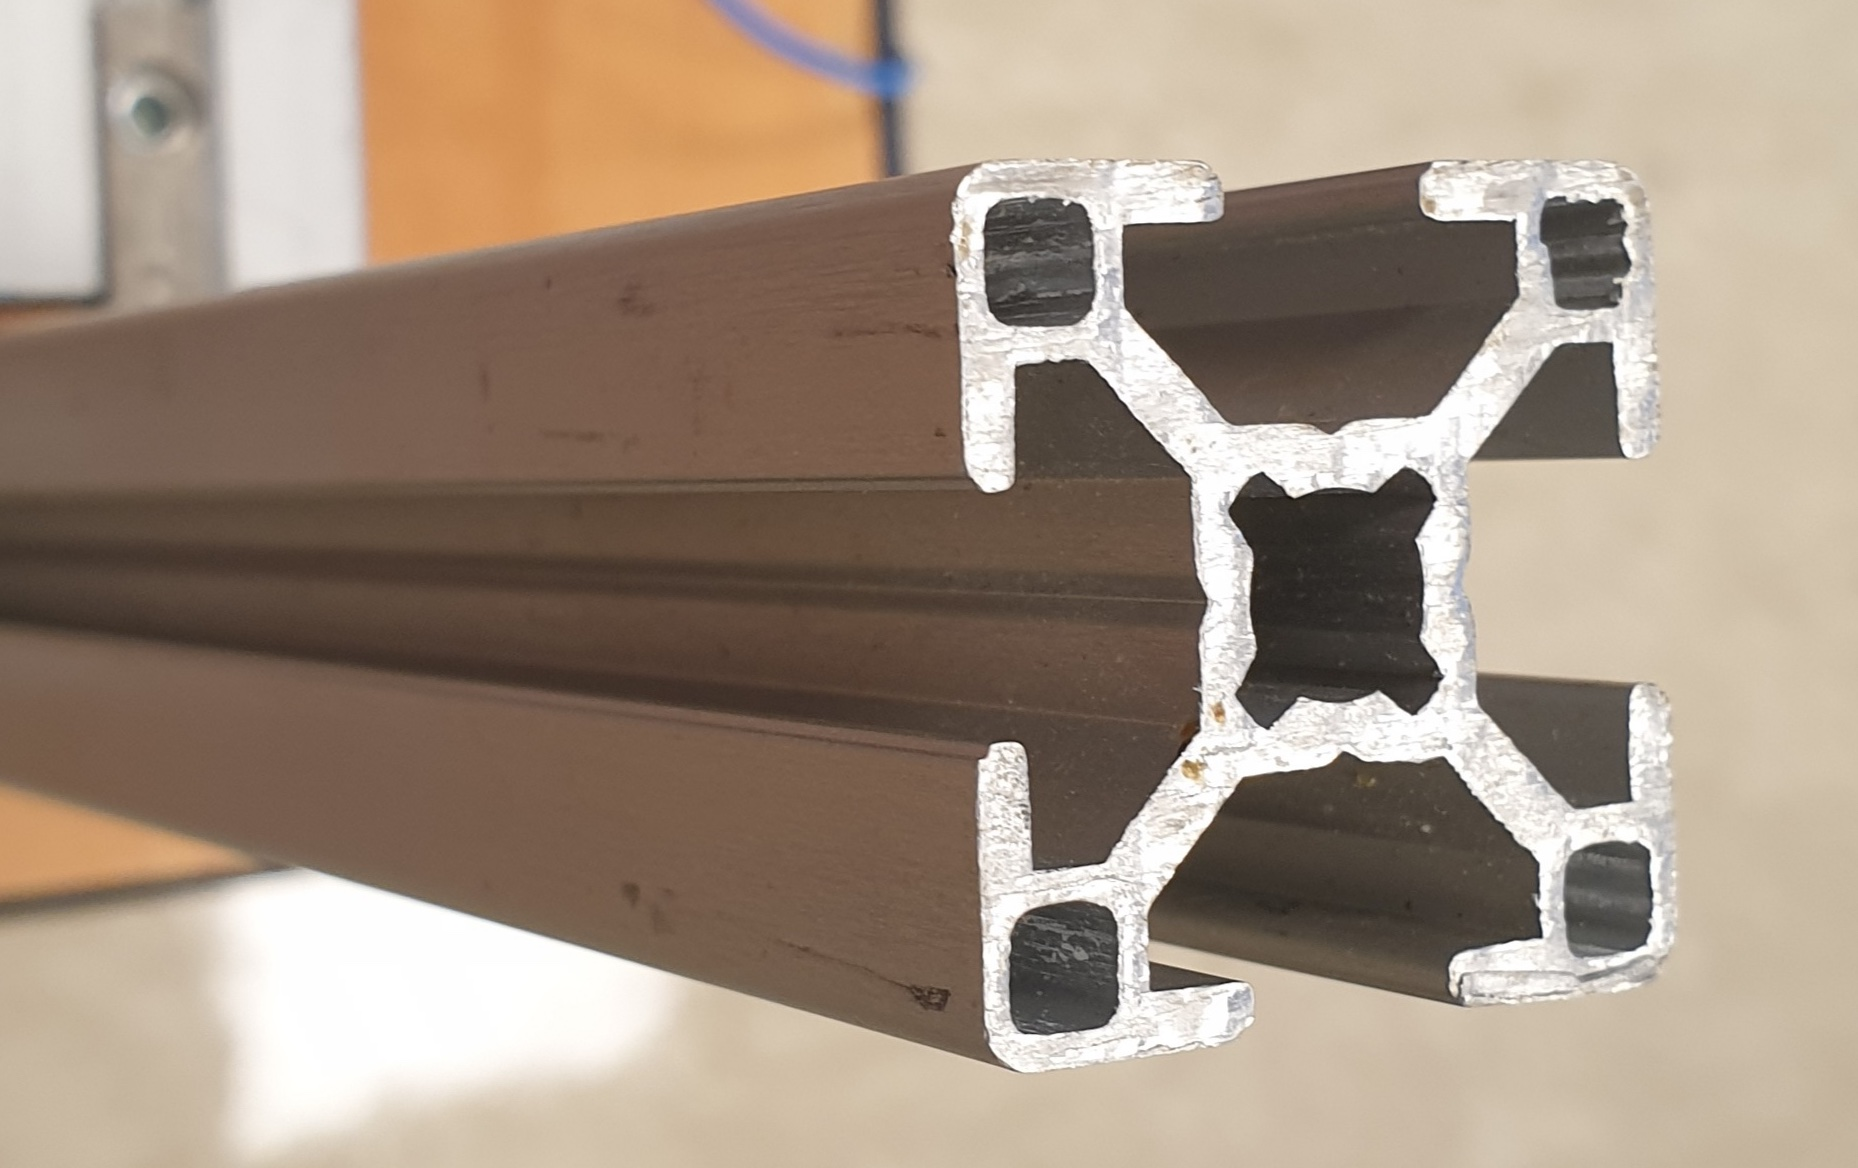
\includegraphics[width=6cm]{FigurasMemoria/perfiles.jpg}
    \caption{Perfiles de aluminio utilizados en la estructura.}
    \label{fig:perfiles} %Para referenciar -> \ref{fig:figNum}
\end{figure}

La ventaja de utilizar estos perfiles es que se puede modificar de manera muy sencilla la distribución de las diferentes partes del montaje, las cuales consisten en: dos parejas de perfiles en \textbf{T} que sirven de apoyo para el resto de la estructura, un perfil inferior que es en el que se coloca la bobina y un perfil superior que es en el que se colocan los sensores de movimiento y el circuito electrónico.

\subsection{Sensores de movimiento}
\label{subsec:sensoresmov}

Los sensores de movimiento utilizados para el proyecto tienen como objetivo proporcionar la diferencia temporal que se utilizará para el cálculo de la velocidad de salida del vástago. Los sensores que se han empleado son sensores de carácter capacitivo, lo que significa que detectan la presencia de un objeto delante de ellos por el cambio de la capacidad con la superficie del sensor. Colocando dos de estos dispositivos a una distancia conocida \textit{d} y obteniendo la diferencia temporal \(\Delta t\) de activación de la señal mediante una placa arduino conectada al sistema, es trivial calcular la velocidad del vástago según la fórmula:

\[v_{vas}=\frac{d}{\Delta t}\]

Los sensores elegidos para llevar a cabo esta tarea son los GLV12-8-200/37/40b/115, los cuales tienen el siguiente esquema de conexión:

\begin{figure}[H]
    \centering
    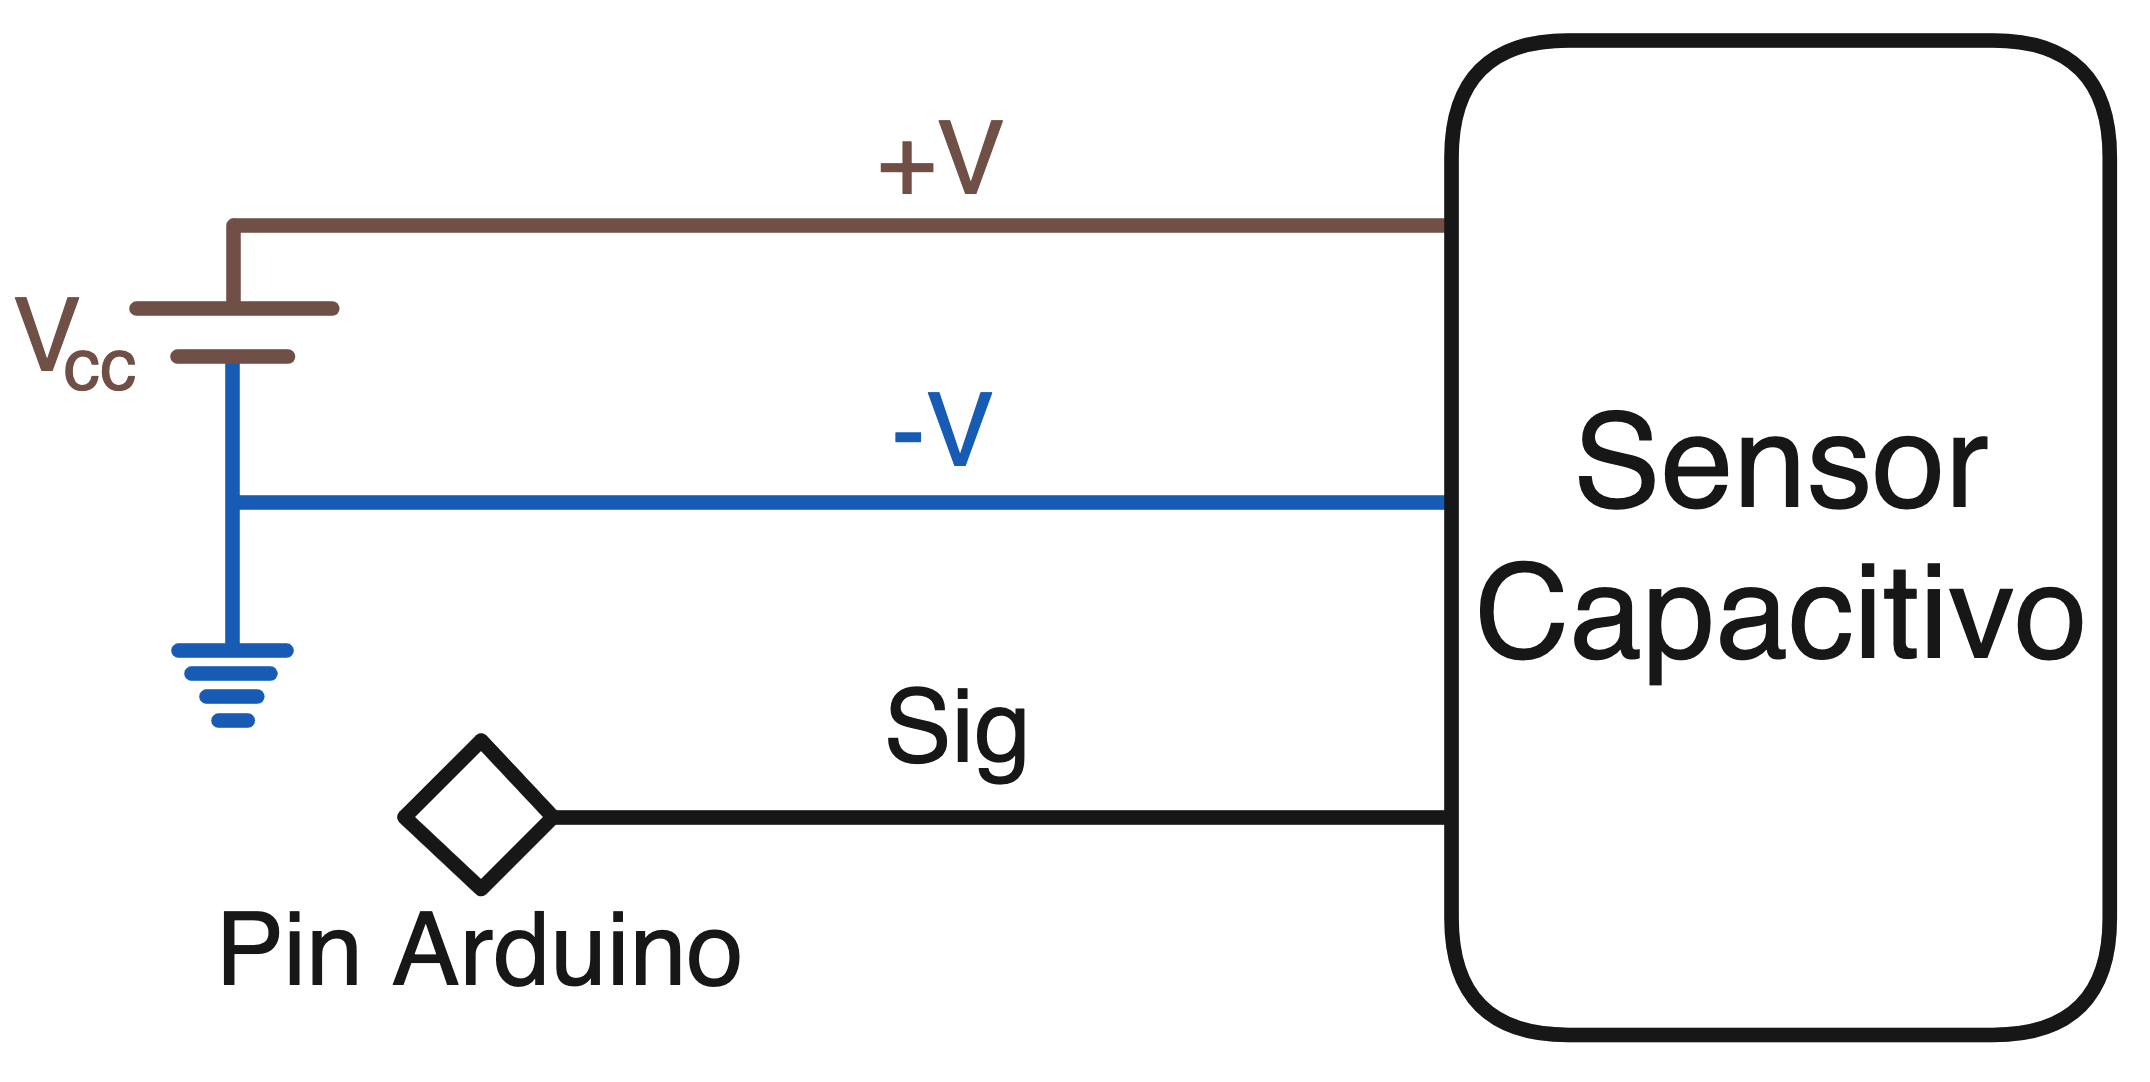
\includegraphics[width=10cm]{FigurasMemoria/esquemaSensor.png}
    \caption{Esquema conexiones de los sensores capacitivos.}
    \label{fig:esquemaSensor} %Para referenciar -> \ref{fig:figNum}
\end{figure}

Observando las especificaciones de este modelo detalladas en las \textit{datasheets} al final del documento, encontramos que la tensión de alimentación del sensor es de \(V_{cc}\in [10,~30]~\text{V}\), y la salida de la señal (tensión entre \textbf{SIG} y \textbf{GND}) es de \(V_{sig}=V_{cc}\). Esto es algo a tener en cuenta, pues la entrada de los puertos de arduino no puede superar los 5 V y los sensores deben ser alimentados al menos a 5 V. Montando el prototipo, se decidió que el circuito electrónico iba a estar alimentado a 15 V, por lo que será necesario un divisor de tensiones para poder leer la señal de los sensores, el cual está detallado en el siguiente apartado.

\subsection{Circuito electrónico}
\label{subsec:circuito}
El diseño y desarrollo de la lanzadera electromagnética no solo requiere de la implementación de los componentes físicos de soporte, bobina y vástago, sino que también es esencial el diseño de un circuito electrónico que controle y optimice su funcionamiento. La precisión y eficiencia del dispositivo dependen en gran medida de la electrónica que lo acompaña. Durante el proceso de montaje del banco de pruebas, se han identificado dos etapas críticas de las cuales se debe encargar el circuito electrónico: la etapa de disparo y la etapa de medición.

\subsubsection*{Disparo}

Para el disparo, debemos indentificar dos momentos críticos, los de inicio y finalización de alimentación de la bobina para que el vástago adquiera inercia sin quedarse atascado en el campo magnético. Cuando se empezó el proyecto se pensó en realizar los disparos a mano apagando y encendiendo la fuente del solenoide, pero al realizar las simulaciones, se descubrió la imposibilidad de este método ya que la constante de tiempo (\(\tau\)) del sistema ronda los \(10^{-2}~s\) o \(10~ms\). Esto plantea un problema a la hora de disparar el vástago, pues debemos alimentar la bobina por un período de tiempo muy breve, lo cual es imposible de hacer manualmente con repetitividad. Es necesario por ende diseñar de manera electrónica las órdenes de inicio y finalización del disparo del vástago.

El inicio del disparo es trivial, y tratará de un interruptor conectado a la placa arduino. Esta detectará la pulsación del interruptor y mandará la orden de disparo a través del mecanismo correspondiente.

\begin{figure}[H]
    \centering
    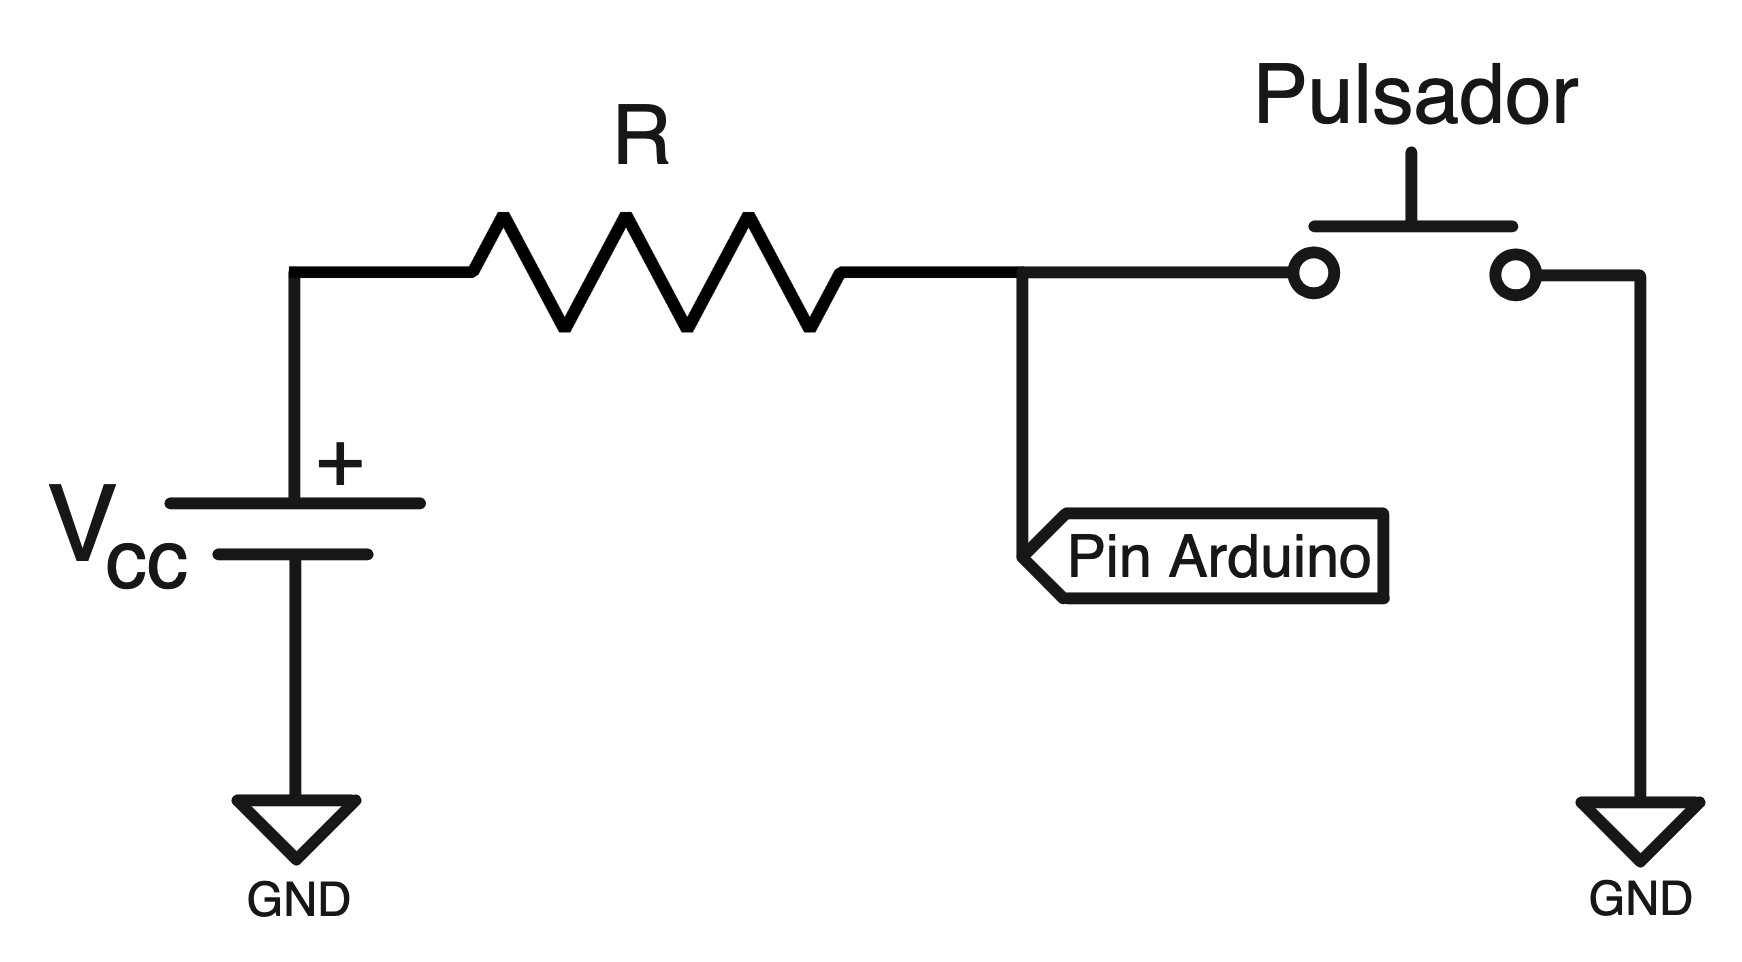
\includegraphics[width=9cm]{FigurasMemoria/conexionInterruptor.png}
    \caption{Conexión del interrupor de disparo.}
    \label{fig:conexionInterruptor} %Para referenciar -> \ref{fig:figNum}
\end{figure}

Por otro lado, la finalización del disparo es más compleja. Es necesario dejar de alimentar la bobina antes de que su centro esté alineado con el del vástago, ya que de lo contrario, este seguirá siendo atraído por el campo magnético y no adquirirá la inercia necesaria para que su movimiento continúe. Para lograr esto, se impondrá la restricción de que \(l_{fe}~<~l_c\) en las dimensiones del sistema. Si colocamos uno de los sensores justo a la salida del solenoide, se podrá obtener la señal de detección del primer sensor antes de que los centros estén alineados, permitiendo que el arduino pueda cortar la corriente en el momento exacto para que el vástago no pierda velocidad.

\begin{figure}[H]
    \centering
    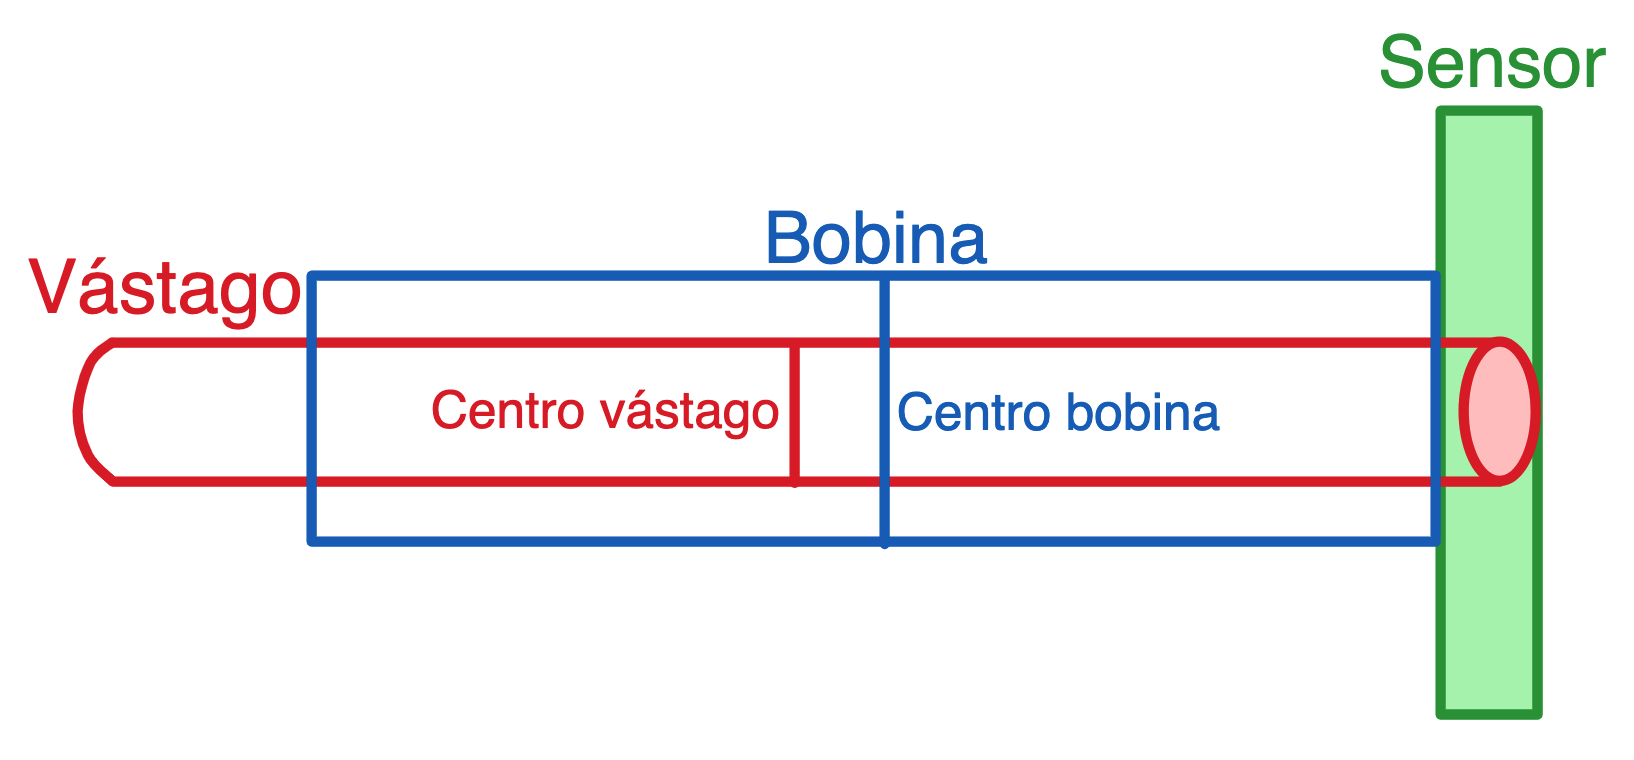
\includegraphics[width=10cm]{FigurasMemoria/esquemaJustDisparo.png}
    \caption{Colocación del sensor.}
    \label{fig:esquemaJustDisparo} %Para referenciar -> \ref{fig:figNum}
\end{figure}

La señal generada por el sensor de movimiento será enviada al Arduino, que la procesará y activará un relé de potencia de estado sólido conectado a uno de sus pines. Este relé estará a su vez conectado a una fuente de corriente y será responsable de interrumpir la alimentación de la bobina en el momento adecuado. El uso de un relé de estado sólido (\textit{solid state relay} o \textit{SSR}) asegura una conmutación rápida y precisa, eliminando la alimentación de la bobina de manera efectiva y asegurando el correcto funcionamiento del sistema de disparo. Con un sistema de corte asegurado, el disparo del proyectil queda resuelto.

\begin{figure}[H]
    \centering
    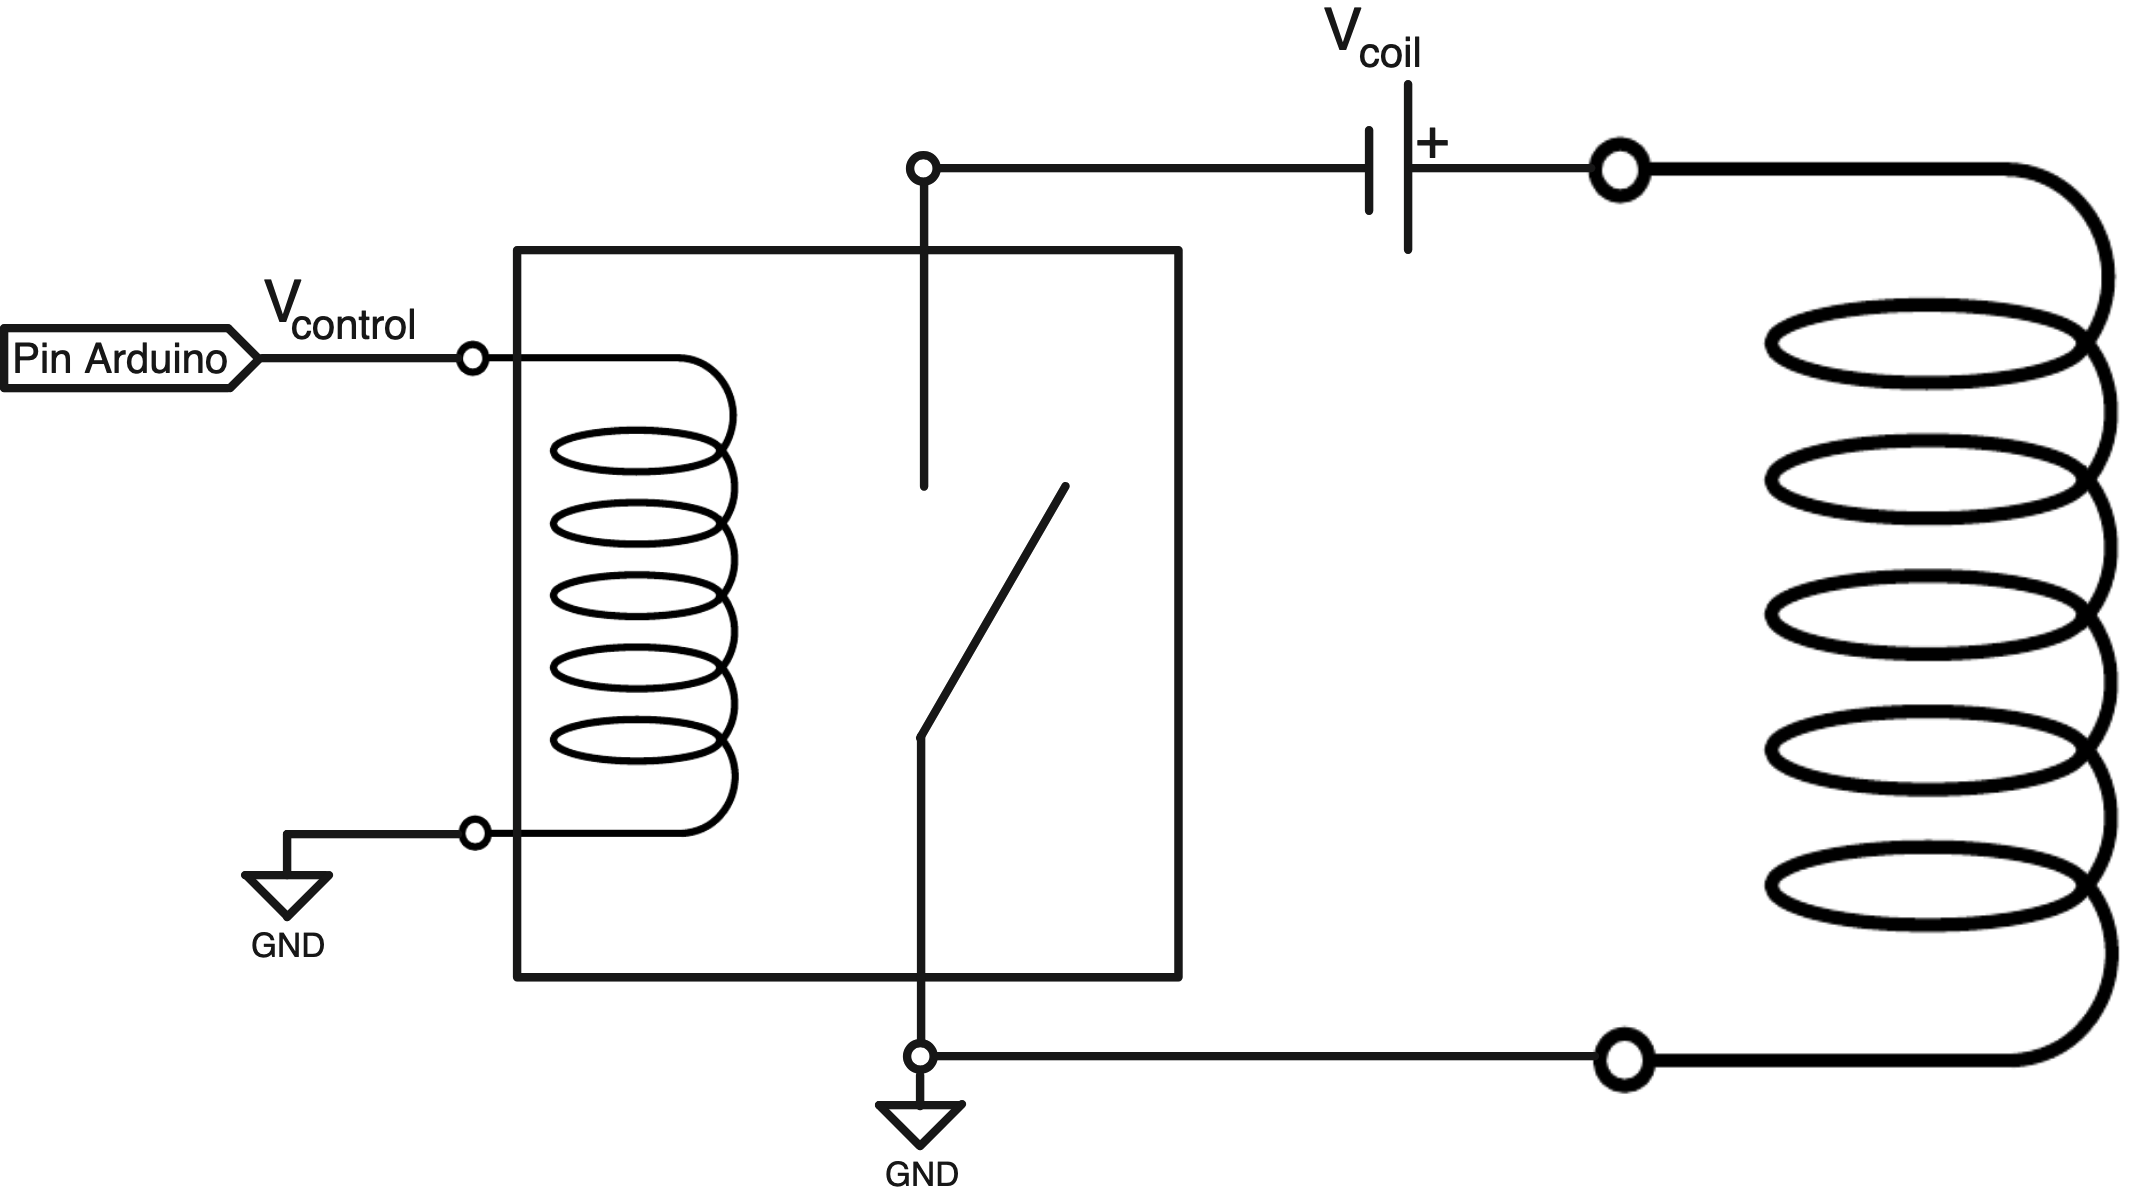
\includegraphics[width=10cm]{FigurasMemoria/conexionRele.png}
    \caption{Esquema eléctrico de la conexión del SSR.}
    \label{fig:conexionRele} %Para referenciar -> \ref{fig:figNum}
\end{figure}

El SSR elegido para el proyecto es el KSJ100D20-L(068). Su tensión de control es de \(V_{control}\in [4,~32]~V\) y la carga que soporta se encuentra en \(S_{pow}\leq 100~\text{VA}\). En el circuito se va a implementar un relé auxiliar por si el SSR se cambia y fuera necesaria una tensión de control superior a 5 V, la cual el arduino no podría proporcionar. Este relé auxiliar es un PRMA1A05, al cual se le conectaría la tensión de alimentación de los sensores a la entrada del interruptor y la etapa de control del SSR a la salida del mismo.


\begin{figure}[H]
    \centering
    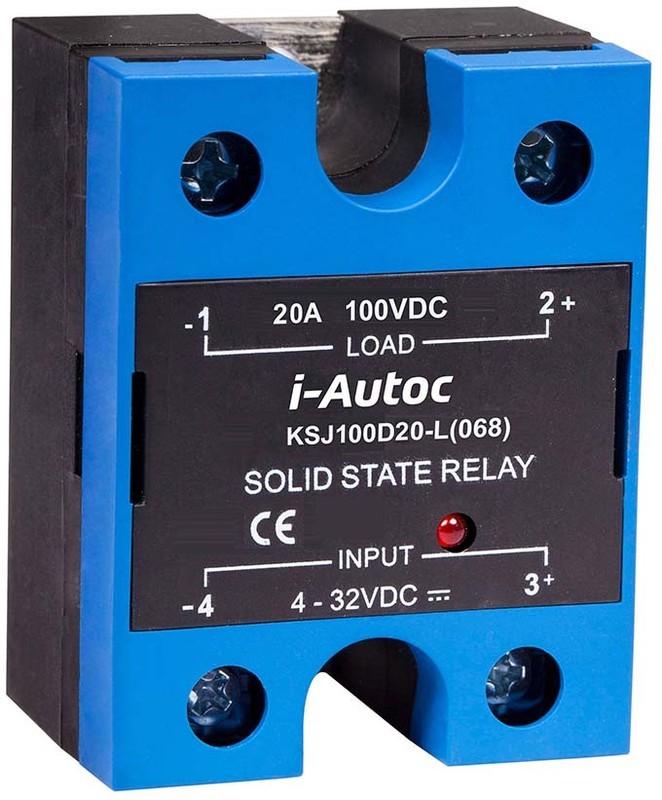
\includegraphics[width=4cm]{FigurasMemoria/SSRrelay.jpeg}
    \caption{Imagen del relé de estado sólido \citep{rs2024ksj}.}
    \label{fig:SSRrelay} %Para referenciar -> \ref{fig:figNum}
\end{figure}

\begin{figure}[H]
    \centering
    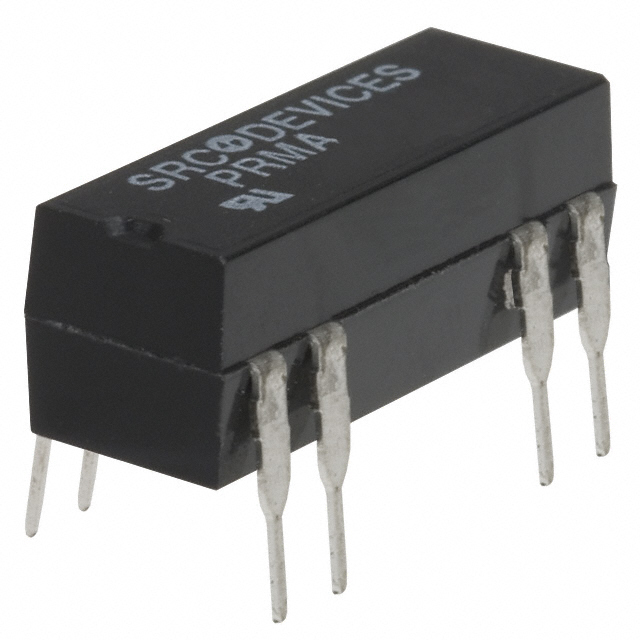
\includegraphics[width=4cm]{FigurasMemoria/PRMArelay.jpeg}
    \caption{Imagen del relé PRMA1A05 \citep{coto2024prma1a05b}.}
    \label{fig:PRMArelay} %Para referenciar -> \ref{fig:figNum}
\end{figure}

\subsubsection*{Medición}

El siguiente y último paso para completar el circuito electrónico es la conversión de la tensión de salida de la señal del sensor de movimiento a un nivel apto para el Arduino para poder realizar la medición. Para ello, se utilizará un divisor de tensiones que debe disminuir la tensión de 15V a 5V. Teniendo en cuenta la estructura de esta configuración, obtenemos lo siguiente:

\begin{figure}[H]
    \centering
    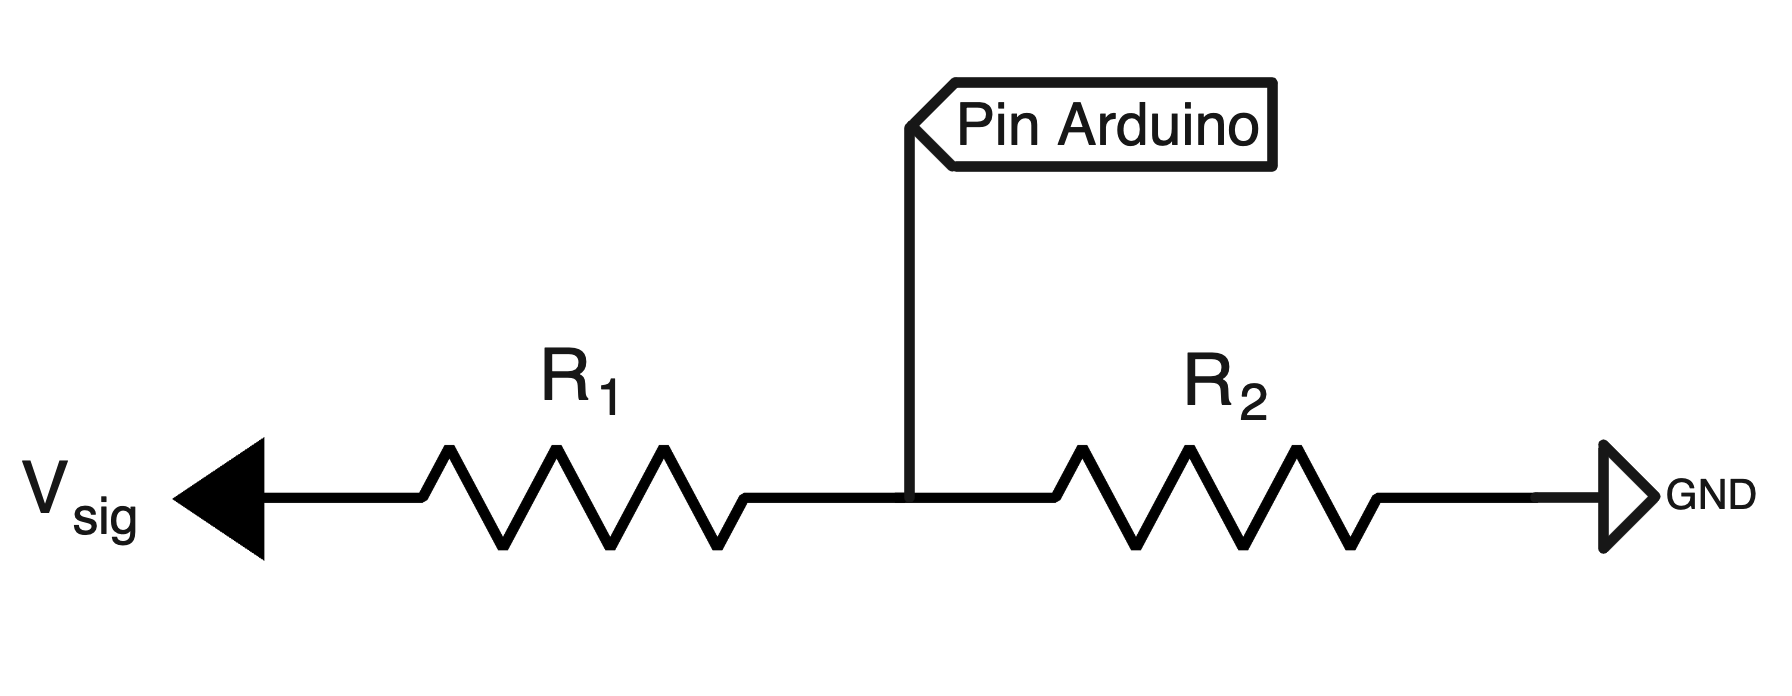
\includegraphics[width=10cm]{FigurasMemoria/divisorTensiones.png}
    \caption{Esquema eléctrico de un divisor de tensiones.}
    \label{fig:divisorTensiones} %Para referenciar -> \ref{fig:figNum}
\end{figure}
\[
V_{pin}=\frac{R_2}{R_1+R_2}V_{sig}
\]
\[
V_{pin}=\frac{1}{4}V_{sig}\to \frac{R_2}{R_1+R_2}=\frac{1}{4}\to 4R_2=R_1+R_2\to R_1=3R_2
\]

Eligiendo \(R_1=10~k\Omega\) para que las corrientes sean del orden de \(10^{-3}~A\), nos queda que \(R_2=3~k\Omega\). Estas resistencias no existen de manera estandarizada por lo que se utilizarán resistencias de un valor de \(R_2=2.7~k\Omega\).

\newpage
\subsubsection*{PCB}

Teniendo en cuenta todas las etapas mencionadas en esta sección, se ha diseñado una PCB para colocar en el banco de pruebas y poder hacer el control oportuno de la bobina. El esquemático queda tal que:

\begin{figure}[H]
    \centering
    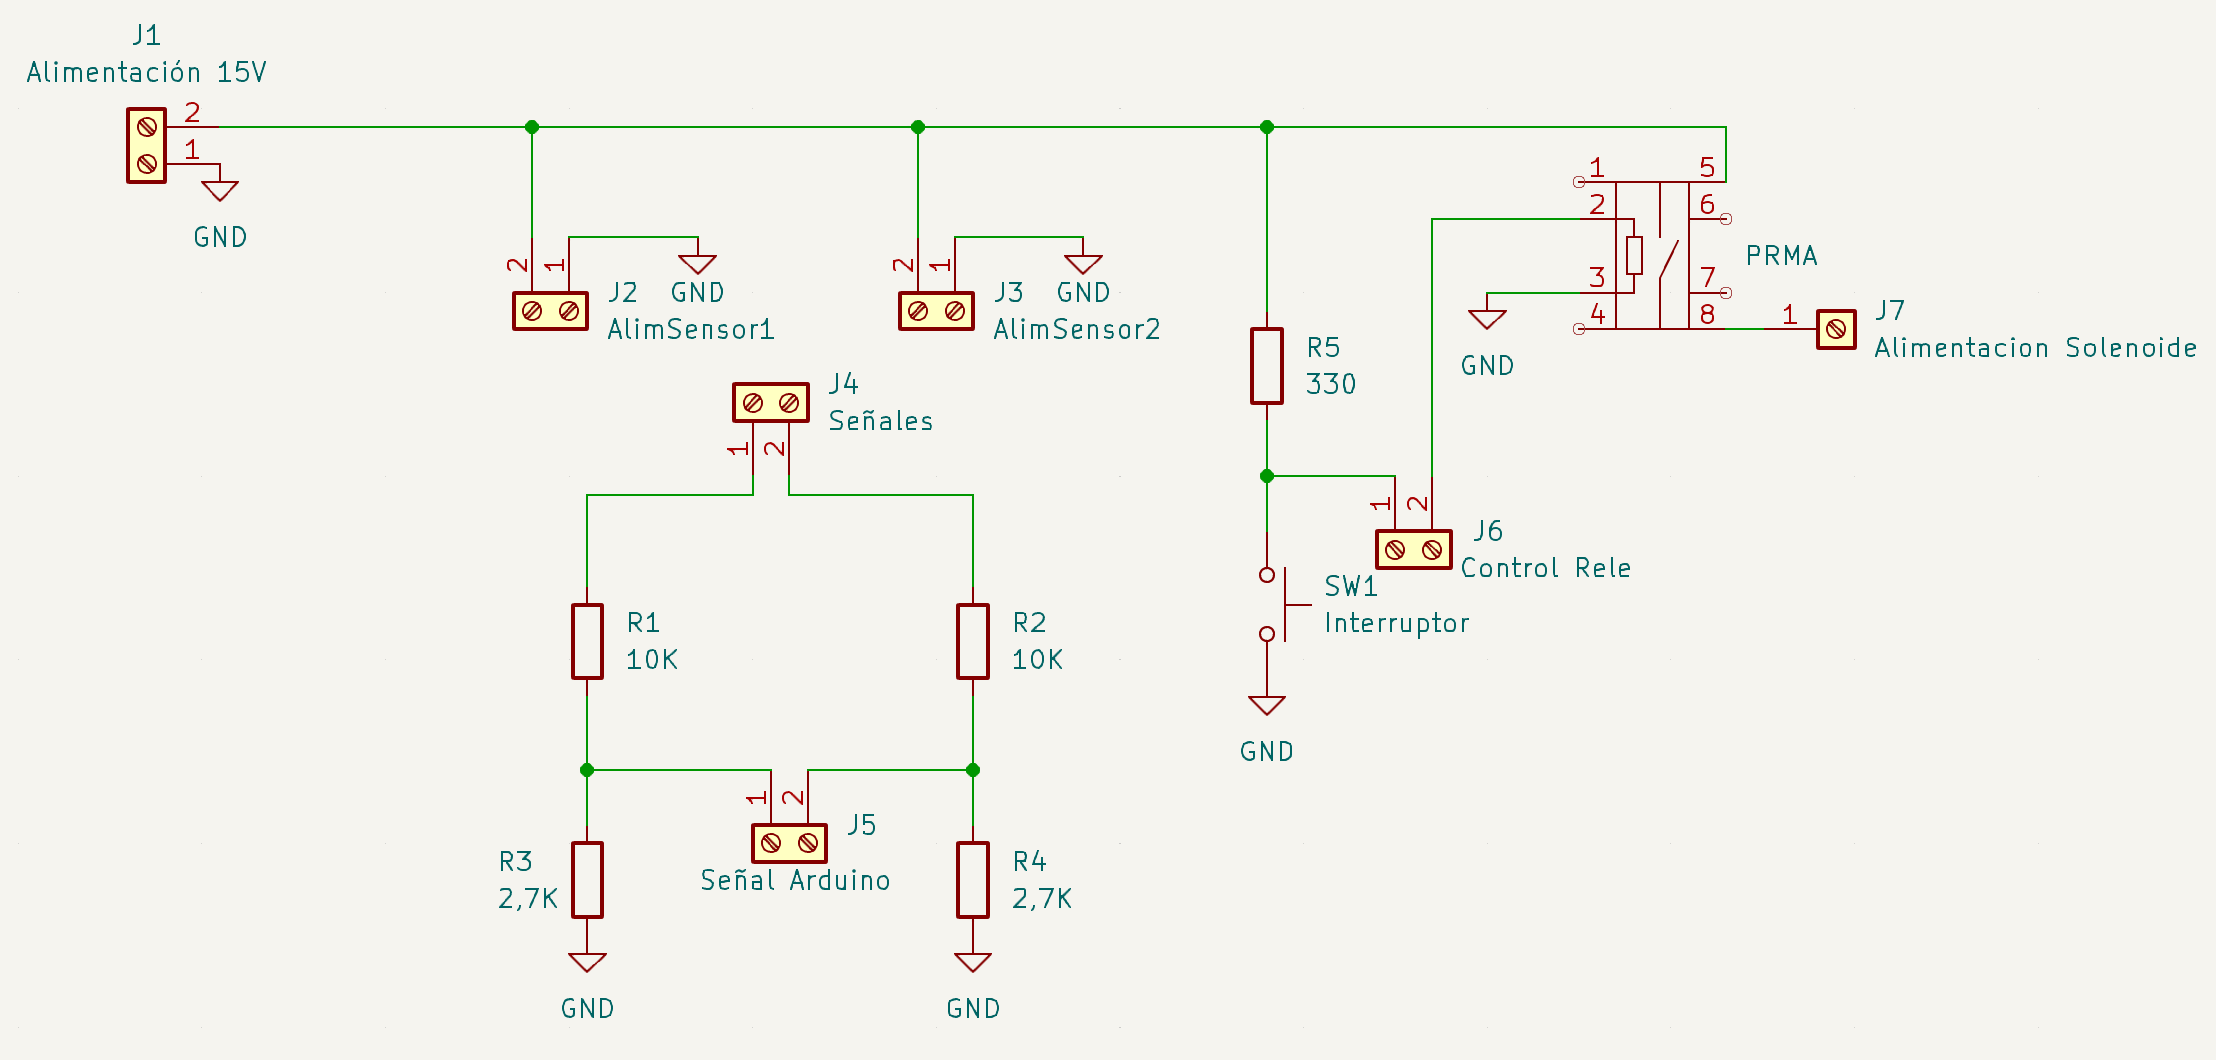
\includegraphics[width=\linewidth]{FigurasMemoria/esquematicoPCB.png}
    \caption{Esquemático de la PCB del proyecto.}
    \label{fig:esquematicoPCB} %Para referenciar -> \ref{fig:figNum}
\end{figure}

\noindent Y la distribución de la placa queda:

\begin{figure}[H]
    \centering
    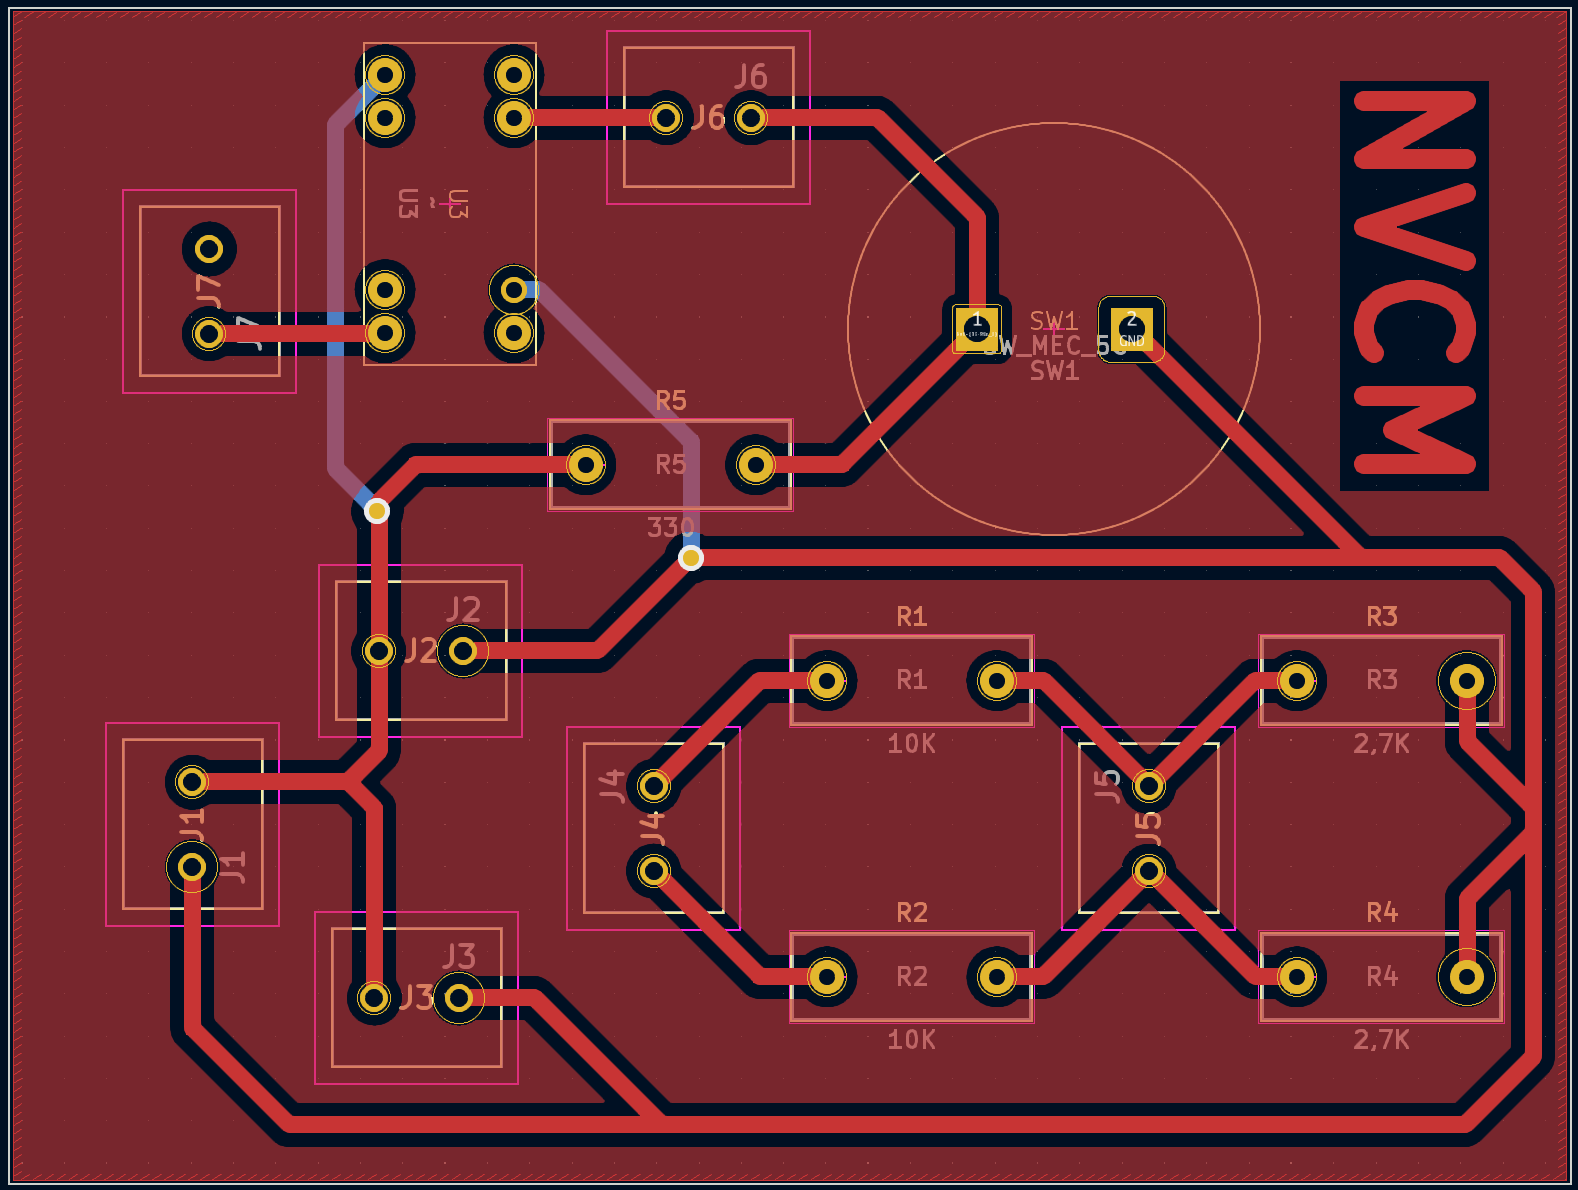
\includegraphics[width=12.5cm]{FigurasMemoria/placaPCB.png}
    \caption{Distribución de la placa del proyecto.}
    \label{fig:placaPCB} %Para referenciar -> \ref{fig:figNum}
\end{figure}

El relé \textit{U3} que se observa en los esquemas es el PRMA1A05. Esta PCB irá conectada a un Arduino Leonardo en los pines de salida que se observan en la figura \ref{fig:esquematicoPCB}, y el código de control se encuentra en el Anexo II.

\subsection{Diseño de la bobina}
\label{subsec:bobina}

Los solenoides que se prueben en el prototipo deben de cumplir las siguientes especificaciones:

\begin{itemize}
    \item \(0.5\leq l_{c} \leq XX\): la longitud máxima de la bobina está delimitada por la longitud del perfil menos un espacio mínimo entre sensores.
    \item \(l_c~<~l_{fe}\): como se ha desarrollado en el apartado anterior, será necesario que la longitud de la bobina sea menor que la del vástago para que el sistema de medición funcione.
    \item \(r_{cint} > r_{fe}\): es evidente que el radio interior de la bobina debe ser mayor que el del vástago para permitir que este último pueda desplazarse en su interior.
    \item \(r_{cext} < XXX\): debido a la disposición de los perfiles de aluminio, hay un radio máximo para que la bobina entre en el banco de pruebas.
\end{itemize}

En cuanto al solenoide del banco de pruebas, solo queda un aspecto por valorar. Aunque hasta el momento no se ha considerado, es crucial para el diseño de una bobina tener en cuenta el radio de la sección del cobre (\(r_{cu}\)), ya que este determinará la cantidad de corriente que la bobina puede soportar dentro de los límites térmicos del material, así como sus dimensiones. Este radio del cobre hace que el radio externo de la bobina se convierta en un parámetro dependiente, por lo que ya no será un valor de diseño a elección del alumno. Los estudiantes que realicen la práctica deberán evaluar la cantidad de corriente y el número de espiras que desean implementar, y seleccionar una sección de cobre que les proporcione un \(r_{cext}\) dentro del límite especificado al inicio de esta sección. Para comprobar que efectivamente el radio cumple con las restricciones, se desarrollará una expresión partiendo de \(N,~r_{cu},~r_{int}~\text{y}~l_c\) como variables conocidas:

\begin{figure}[H]
    \centering
    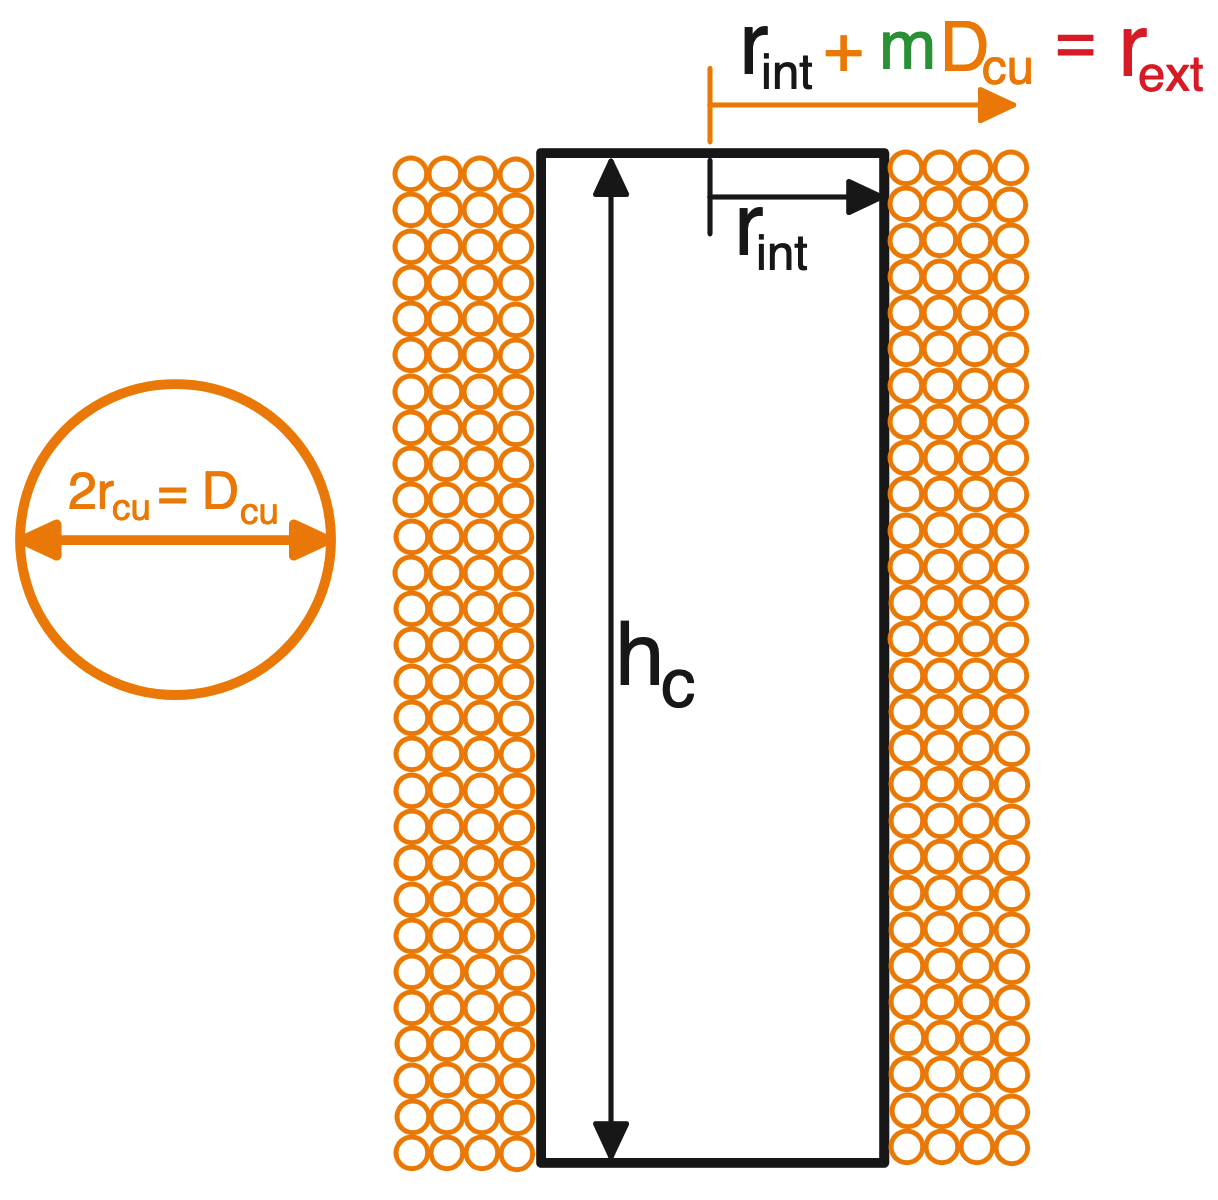
\includegraphics[width=7cm]{FigurasMemoria/esquemaBobinaREXT.png}
    \caption{Sección central del solenoide.}
    \label{fig:esquemaBobinaREXT} %Para referenciar -> \ref{fig:figNum}
\end{figure}

El objetivo es conseguir el parámetro \textit{m}, que se corresponde con el número de capas que van a envolver a \(r_{int}\) y contendrán \(N\) espiras. El primer paso será obtener el número de conductores en cada capa, que se puede escribir como el truncamiento del cociente entre la longitud de la bobina y el diámetro de los conductores:

\[\text{nº~de~conductores~por~capa}=t=\frac{l_c}{D_{cu}}=\frac{l_c}{2r_{cu}}\]

El número de capas será por tanto el número de espiras entre este valor:

\[m=\frac{N}{t}=\frac{ND_{cu}}{l_c}\]

Y el radio exterior queda:

\[r_{ext}=r_{int}+mD_{cu}=r_{int}+\frac{ND_{cu}^2}{l_c}=r_{int}+4\frac{Nr_{cu}^2}{l_c}\]

Podemos comprobar la efectividad de la fórmula con la bobina de prueba del proyecto, para la que:

\[N=500~~~~~~r_{cu}=0.8~mm~~~~~~r_{int}=6.035~\text{mm}~~~~~~l_c=53.12~\text{mm}\]

Sustituyendo en la fórmula obtenida:

\[r_{ext~form}=0.006035+\frac{500*(0.8*10^{-3})^2}{0.05312}=0.01206~\text{m}=12.06~\text{mm}\]

Comparando ahora con el valor expuesto en el apartado de cálculo analítico \ref{sec:analitico}:

\[r_{ext~form}=12.06~\text{mm}\approx r_{c}=10.64~\text{mm}\]

Observamos que los valores son bastante similares, con un error del 13\%. Esta diferencia se debe a que en la fórmula estamos asumiendo que el parámetro \textit{t} es igual para todas las capas, lo cual es muy difícil de lograr cuando se bobina un solenoide en la realidad. A pesar de esto, consideramos que el desarrollo proporciona un dato bastante preciso, por lo que se empleará en la práctica como camino para obtener \(r_{ext}\). Se añadirá además al código de MATLAB\textsuperscript{\textregistered}  la opción de poder calcular la fuerza de atracción a partir de este desarrollo. Esto resulta en la siguiente actualización de la interfaz de la calculadora:

\begin{figure}[H]
    \centering
    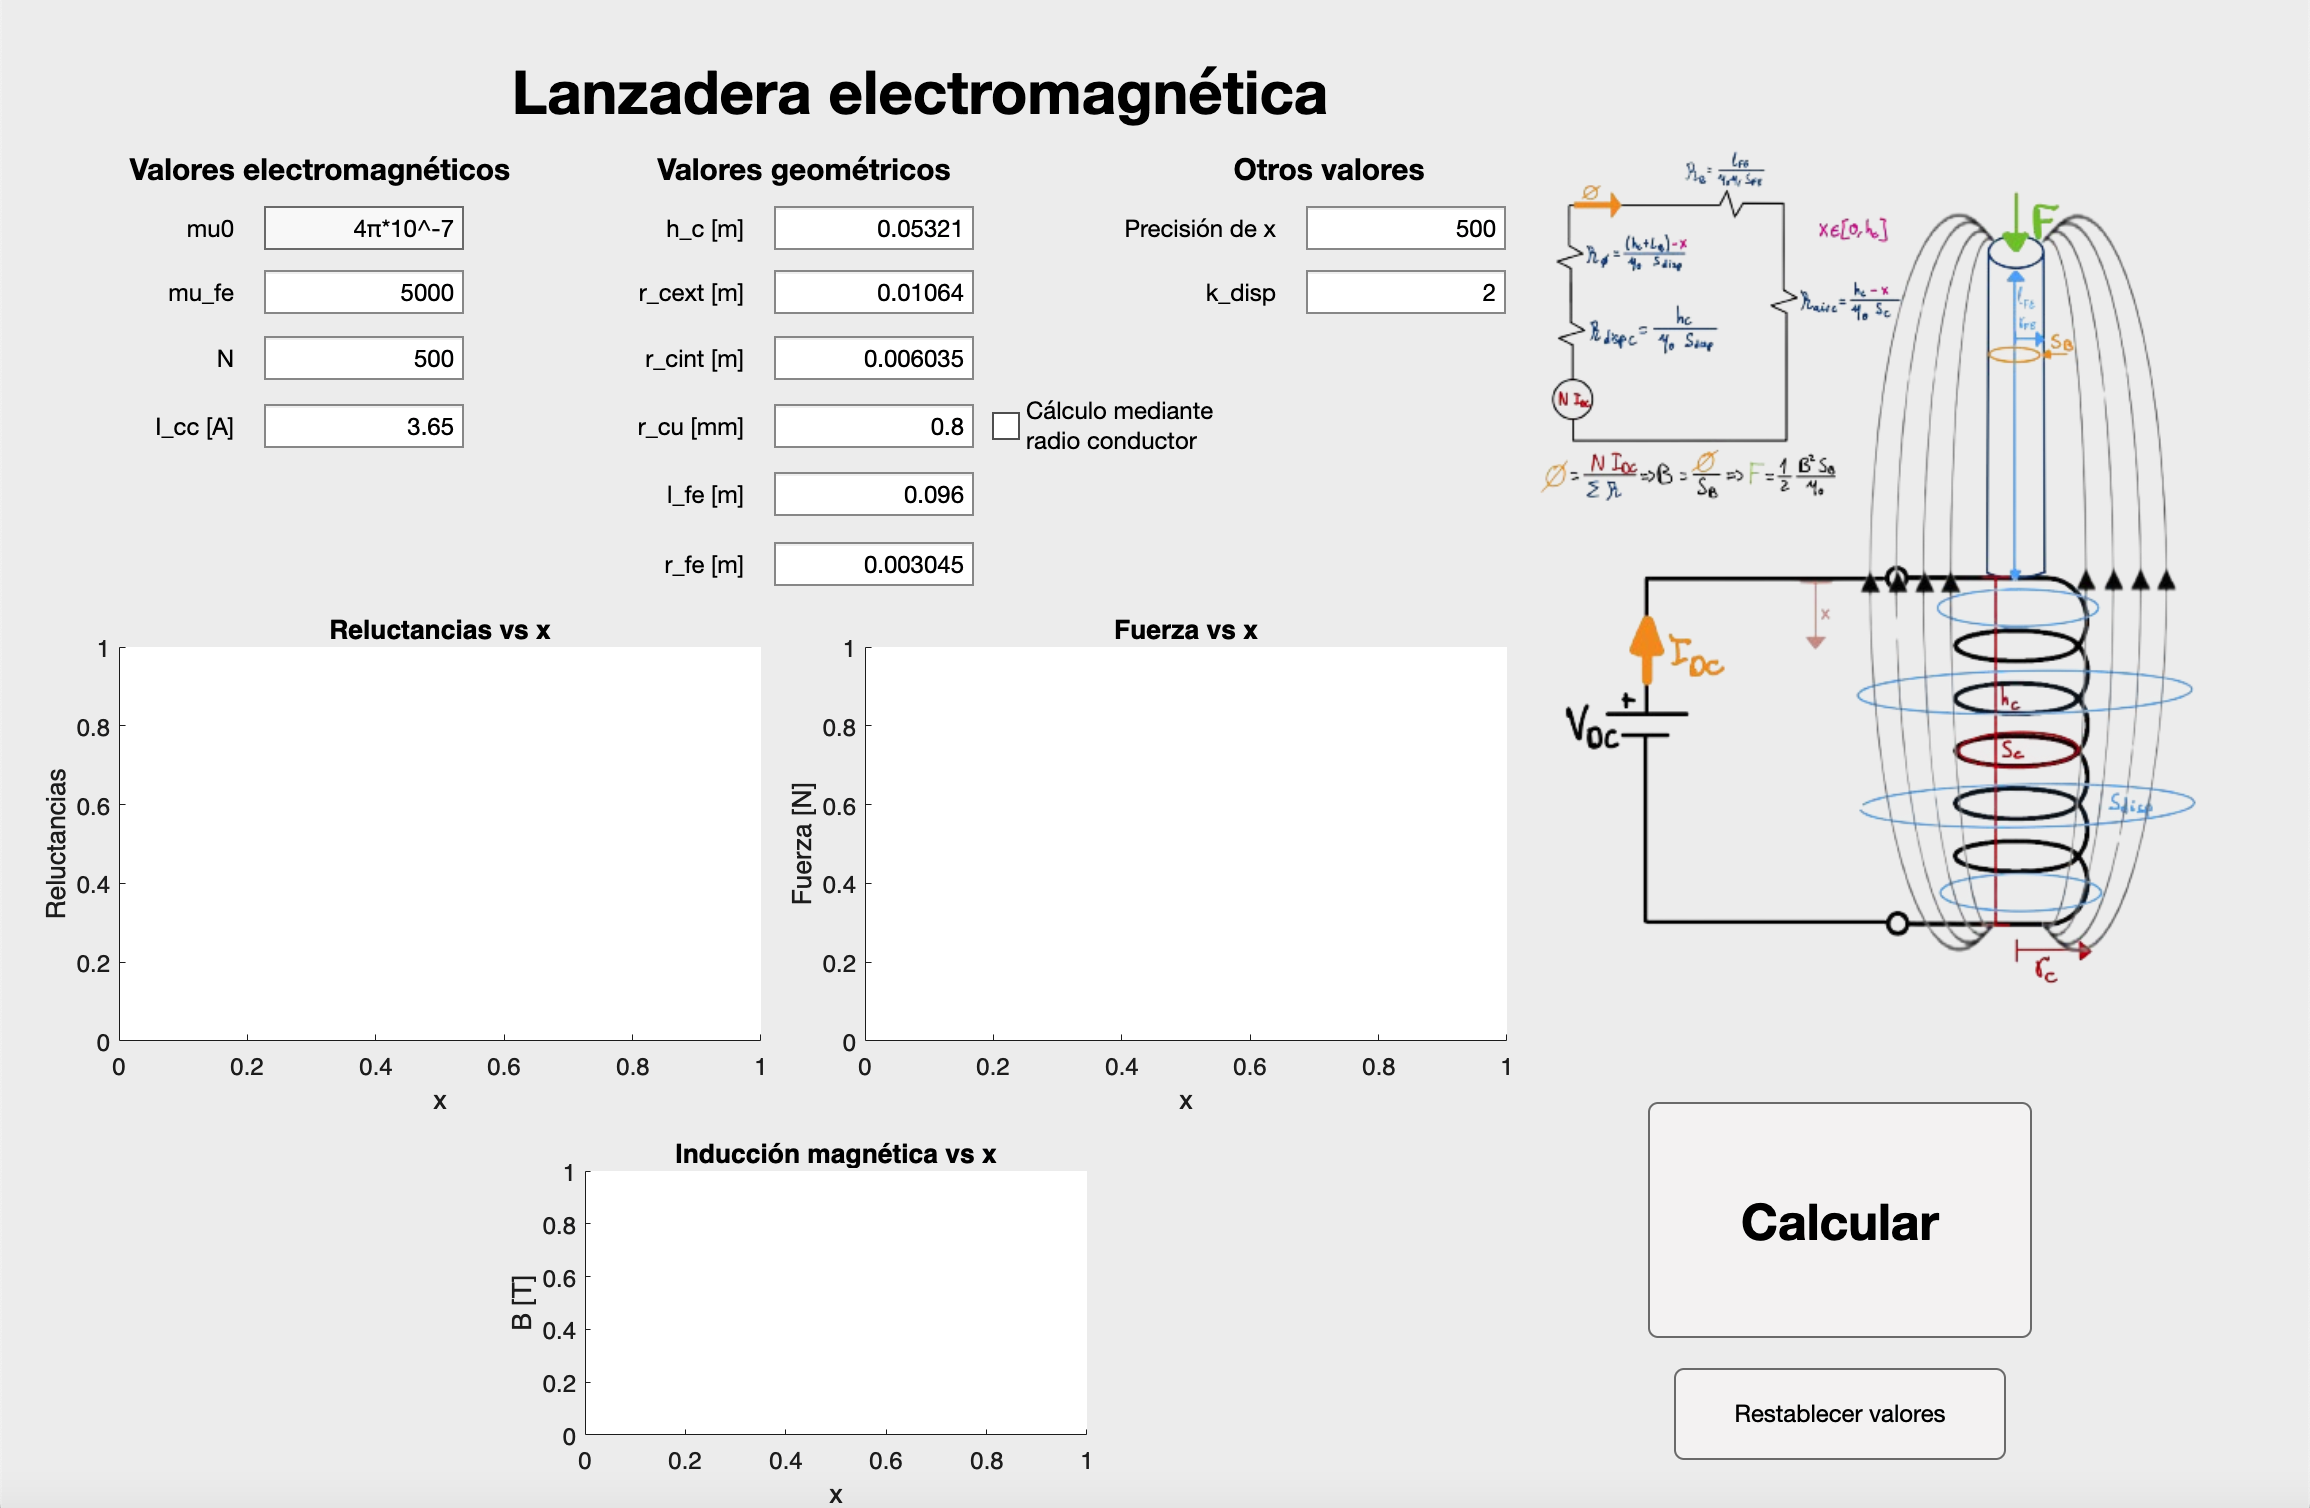
\includegraphics[width=9.5cm]{FigurasMemoria/calculadoraDef.png}
    \caption{Interfaz de la calculadora actualizada.}
    \label{fig:calculadoraDef} %Para referenciar -> \ref{fig:figNum}
\end{figure}

\newpage
\section{Resultados}
\label{sec:resultados}
\subsection{Validación de los modelos}
\label{subsec:validacionModelos}

Esta sección se centrará en validar los diferentes modelos obtenidos en las secciones anteriores, específicamente la calculadora desarrollada en el cálculo analítico (\ref{sec:analitico}) y el modelo de cálculo por elementos finitos (\ref{sec:simulaciones}).

Los resultados de ambos modelos se presentan en forma de gráficas que muestran la evolución de la fuerza de atracción magnética. En el caso del cálculo analítico, la fuerza se expresa en función de la posición del vástago, mientras que en el modelo de elementos finitos, se expresa en función del tiempo. Aunque estas parecen ser variables independientes diferentes, ambas gráficas pueden considerarse análogas, ya que la única variable que varía en el sistema físico es la posición del vástago, midiéndola directamente en el primer modelo y observando su evolución temporal en el otro.

Esto implica que la evolución de la fuerza en ambas gráficas debería ser muy similar. Aunque se ha mencionado anteriormente que la magnitud del cálculo mediante elementos finitos no es precisa, podemos comparar las gráficas de las figuras \ref{fig:calcFsetupBase} y \ref{fig:S3ForceCurrent} para comprobar que, efectivamente, la evolución del parámetro de fuerza de atracción sigue el mismo patrón.

\begin{figure}[htbp]
    \centering
    \begin{minipage}{0.85\textwidth}
        \centering
        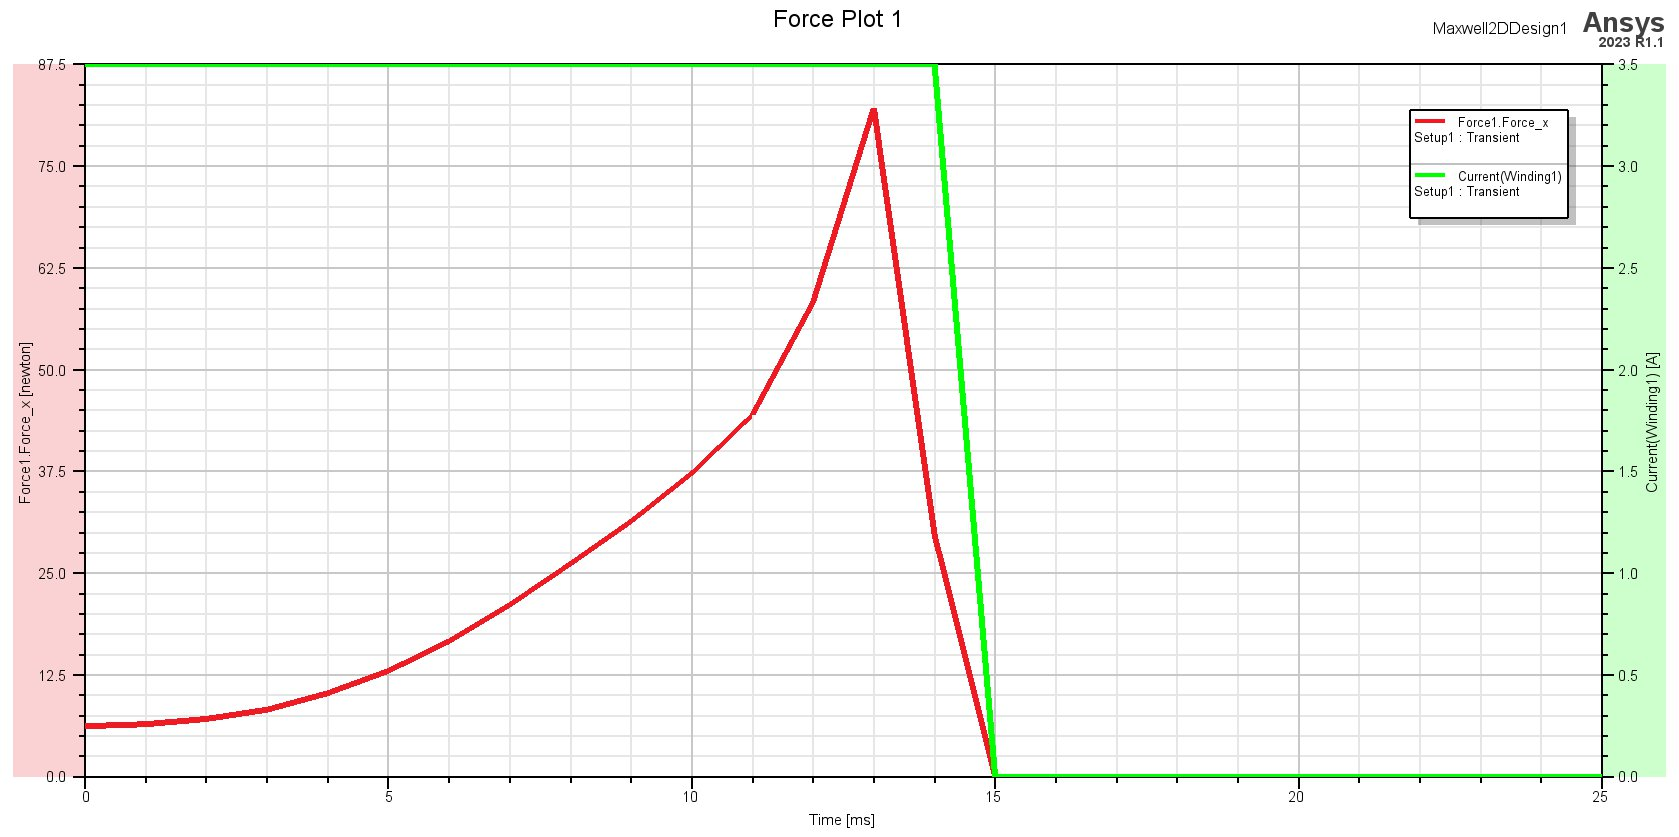
\includegraphics[width=\textwidth]{FigurasMemoria/S3ForceCurrent.jpg}
    \end{minipage}
    \hfill
    \begin{minipage}{0.9\textwidth}
        \centering
        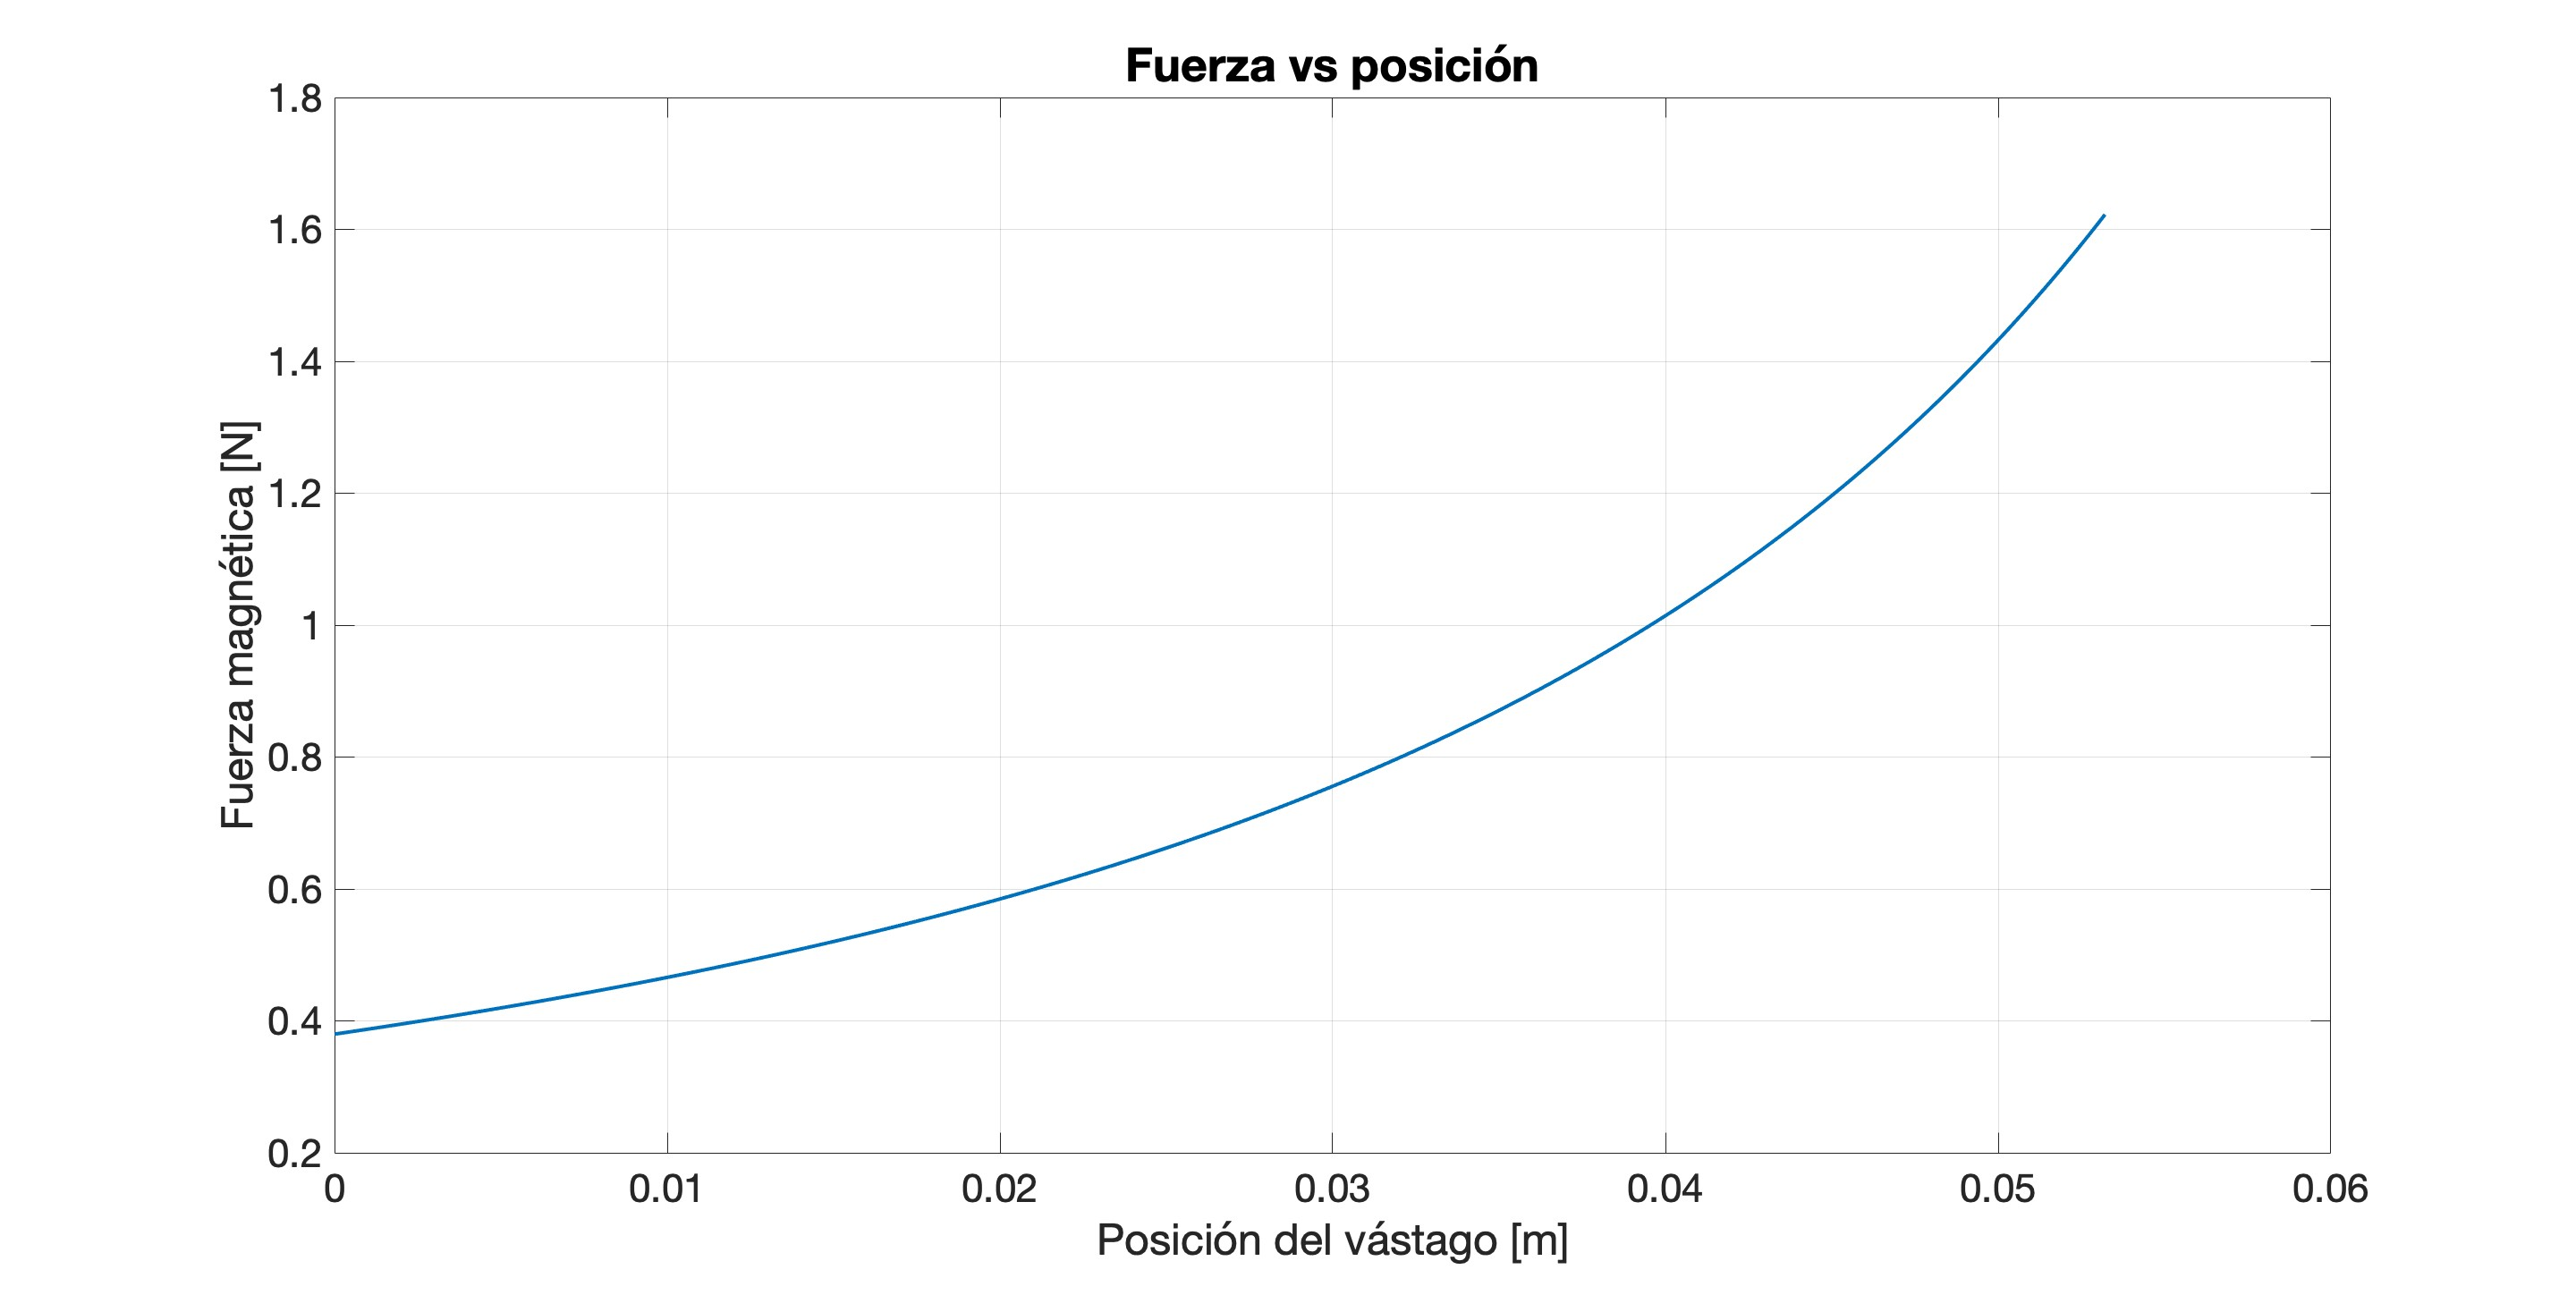
\includegraphics[width=\textwidth]{FigurasMemoria/calcFsetupBase.jpg}
    \end{minipage}
    \caption{Comparación de las figuras \ref{fig:calcFsetupBase} y \ref{fig:S3ForceCurrent}.}
    \label{fig:comparacionF}
\end{figure}

Como observamos en esta figura, la evolución de ambas gráficas muestra una curva ascendente, alcanzando el valor máximo de fuerza en el último momento de alimentación de la bobina. La gráfica de la figura \ref{fig:calcFsetupBase} no decrece porque no está computado lo que ocurre después de que \textit{x} llegue a su valor máximo. Sin embargo, este máximo del parámetro de posición del vástago coincide con el cese de la alimentación de la bobina, por lo que la fuerza se haría cero instantes después.

Como última observación, se puede notar en la gráfica del cálculo por elementos finitos que, al estar en un orden de magnitud de tiempo tan pequeño, ocurre un estado transitorio desde que la fuente deja de proporcionar corriente a la bobina hasta que esta realmente deja de emitir campo magnético. Esto se debe a la expresión de la evolución de la tensión y corriente en un solenoide:

\[V_L=L\frac{\partial i}{\partial t}\]

Lo que indica que existe una resistencia a la desaparición de la corriente en estos dispositivos debido a su tendencia de retener campo magnético.

Dado que el modelo analítico proporciona una aproximación mucho más certera tanto del valor de la fuerza como de su evolución, se concluye que ha sido exitoso su desarrollo y será el que se presente a los alumnos como método de comprobación de su elección de parámetros en el apartado de la práctica (\ref{sec:practica}).

\subsection{Resultados del prototipo}
\label{subsec:prototipoResults}

Los resultados del prototipo consisten en una serie de mediciones con diferentes valores de alimentación para la bobina de prueba. Se detallarán a continuación las diferentes configuraciones probadas y se discutirá si se puede explicar efectivamente las variaciones con el modelo propuesto en el apartado anterior. Las alimentaciones del prototipo son:

\newgeometry{left=1.5cm, right=1.5cm, top = 2.5cm, bottom = 2.5cm}

\begin{table}[H]
    \centering
    \setlength{\tabcolsep}{5pt}
    \renewcommand{\arraystretch}{1.2}
    \begin{tabular}{|c|c|c|c|}
        \hline
        \textbf{Alimentación} & \textbf{Tensión [V]} & \textbf{Resistencia [\(\Omega\)]} & \textbf{Corriente [A]}\\
        \hline
        1 & 13,1 & 3,5 & 3,74 \\
        2 & 20,0 & 3,5 & 5,71 \\
        3 & 29,7 & 3,5 & 8,49\\
        \hline
    \end{tabular}
    \caption{Denominación de las diferentes alimentaciones.}
    \label{tab:alimentacionesBase}
\end{table}

\begin{table}[H]
    \centering
    \begin{tabular}{|c|c|c|c|c|}
    \hline
    \setlength{\tabcolsep}{5pt}
    \renewcommand{\arraystretch}{1.2}
    \textbf{Alimentación} & \textbf{Tiempo [ms]} & \textbf{Distancia [m]} & \textbf{Velocidad [ms\(^{-1}\)]} & \textbf{Aceleración [ms\(^{-2}\)]} \\
    \hline
    \renewcommand{\tabcolsep}{6pt}
    \renewcommand{\arraystretch}{1.0}
    \multirow{10}{*}{1} & 27     & \multirow{10}{*}{0,0691} & 2,16      & 67,48       \\
                        & 22     &                          & 2,09      & 63,45       \\
                        & 24     &                          & 2,09      & 63,45       \\
                        & 38     &                          & 2,09      & 63,45       \\
                        & 25     &                          & 2,09      & 63,45       \\
                        & 33     &                          & 2,03      & 59,78       \\
                        & 24     &                          & 1,97      & 56,41       \\
                        & 28     &                          & 2,23      & 71,9        \\
                        & 25     &                          & 2,09      & 63,45       \\
                        & 31     &                          & 2,09      & 63,45       \\
    \hdashline[2pt/5pt]
    \multirow{10}{*}{2} & 18     & \multirow{10}{*}{0,0691} & 2,47      & 88,14       \\
                        & 18     &                          & 2,66      & 102,22      \\
                        & 18     &                          & 2,47      & 88,14       \\
                        & 21     &                          & 2,47      & 88,14       \\
                        & 19     &                          & 2,56      & 94,79       \\
                        & 25     &                          & 2,56      & 94,79       \\
                        & 18     &                          & 2,56      & 94,79       \\
                        & 25     &                          & 2,56      & 94,79       \\
                        & 17     &                          & 2,66      & 102,22      \\
                        & 22     &                          & 2,56      & 94,79       \\
    \hdashline[2pt/5pt]
    \multirow{10}{*}{3} & 21     & \multirow{10}{*}{0,0691} & 2,47      & 88,14       \\
                        & 20     &                          & 2,56      & 94,79       \\
                        & 20     &                          & 2,56      & 94,79       \\
                        & 19     &                          & 2,66      & 102,22      \\
                        & 21     &                          & 2,56      & 94,79       \\
                        & 23     &                          & 2,56      & 94,79       \\
                        & 22     &                          & 2,47      & 88,14       \\
                        & 20     &                          & 2,56      & 94,79       \\
                        & 22     &                          & 2,56      & 94,79       \\
                        & 23     &                          & 2,47      & 88,14       \\
    \hline
    \end{tabular}
    \caption{Datos tomados con la bobina base y las alimentaciones de la tabla \ref{tab:alimentacionesBase}.}
    \label{tab:datosBase}
\end{table}

\begin{table}[H]
    \centering
    \setlength{\tabcolsep}{5pt}
    \renewcommand{\arraystretch}{1.2}
    \begin{tabular}{|c|c|c|c|c|}
        \hline
        \textbf{Alimentación} & \textbf{Vel. Media [ms\(^{-1}\)]} & \textbf{Ac. Media [ms\(^{-2}\)]} & \textbf{Fuerza [N]} & \textbf{Fuerza calculada [N]}\\
        \hline
        1 & 2,53 & 92,49 & 1,76 &  1,35\\
        2 & 3,47 & 174,31 & 3,31 & 3,68\\
        3 & 3,28 & 155,8 & 2,96 &  8,31\\
        \hline
    \end{tabular}
    \caption{Resultados del disparo con la bobina base y las alimentaciones de la tabla \ref{tab:alimentacionesBase}.}
    \label{tab:resultadosBase}
\end{table}
\restoregeometry

Analizando las tablas anteriores, podemos observar que a medida que se incrementa la corriente (de 3.74 A en la alimentación 1 a 8.49 A en la alimentación 3), la fuerza calculada también aumenta considerablemente (de 1.35 N a 8.31 N) como es de esperar. Sin embargo, la fuerza medida no sigue el mismo patrón de incremento lineal. Aunque sí aumenta con la corriente, la relación no es directamente proporcional, sugiriendo posibles pérdidas o ineficiencias en el sistema.

Con estos resultados, podemos terminar de validar la simulación ejecutada para obtener las figuras \ref{fig:calcRsetupBase}, \ref{fig:calcBsetupBase} y \ref{fig:calcFsetupBase} y asegurar que el modelo de MATLAB\textsuperscript{\textregistered} proporciona resultados verosímiles con los que se pueden realizar predicciones acertadas.

\section{Práctica propuesta}
\label{sec:practica}

Se presenta a continuación el planteamiento de la práctica a realizar por los alumnos de la asignatura de Sistemas Eléctricos I.

\newpage

\section*{Diseño y optimización de una lanzadera electromagnética}

\subsection*{Objetivo}

El objetivo de esta práctica es que los estudiantes diseñen y construyan la bobina de una lanzadera electromagnética optimizando su geometría y alimentación para lograr la mayor fuerza de atracción magnética y por ende velocidad del proyectil. Se deberán aplicar conocimientos teórico-prácticos de electromagnetismo en tres entornos: MatLab, ANSYS Maxwell y laboratorio.

\subsection*{Marco teórico}

En esta sección se desarrollarán los principios teóricos que permiten el funcionamiento de las lanzaderas electromagnéticas. Para entender estos principios, es esencial comprender los fundamentos del electromagnetismo, el concepto de bobina y su papel en la generación de campos magnéticos.

El comportamiento de las ondas electromagnéticas está definido por las ecuaciones de Maxwell, descritas a continuación:
\begin{figure}[H]
    \centering
    \[
    \vec{\nabla}\cdot \vec{E}= \frac{\rho}{\epsilon_0}~~~~~~\vec{\nabla}\cdot \vec{B}= 0
    \]
    \[
    \vec{\nabla}\times\vec{E}=-\frac{\partial\vec{B}}{\partial t}~~~~~~\vec{\nabla}\times \vec{B}=\mu_0\vec{J}+\mu_0\epsilon_0\frac{\partial \vec{E}}{\partial t}
    \]
\end{figure}

En el caso de esta práctica, la ley de mayor interés es la de Ampère. Esta es la ley que define la relación entre un campo magnético y uno eléctrico, y partir de su forma diferencial expresada en las ecuaciones de Maxwell, se puede desarrollar la ley integral de Ampère como:

\begin{quote}
    "La integral de línea del campo magnético \(\mathbf{B}\) alrededor de un lazo cerrado es igual a \(\mu_0\) multiplicado por la corriente total \(I_{enc}\) que pasa a través de cualquier superficie delimitada por el lazo. Matemáticamente, esto se expresa como:
    \[
    \oint_{\partial S} \mathbf{B} \cdot d\mathbf{l} = \mu_0 I_{enc}
    \]
    donde \(\mu_0\) es la permeabilidad del vacío."
\end{quote}

Esta ley es esencial porque proporciona el punto de partida de la práctica. Debido a que el componente principal de una lanzadera es una bobina, desde la ley integral de Ampère se puede deducir la expresión del campo magnético generado por la misma:

\[B=\mu_0\mu_r\frac{NI}{L}\]

\noindent Siendo:\\
\\ \(B\) valor del campo magnético en [T].\\
\(\mu_0\) valor de la permeabilidad del vacío. Constante e igual a \(4\pi*10^{-7}\) [Hm\(^-1\)].\\
\(\mu_r\) valor de la permeabilidad relativa del núcleo de la bobina.\\
\(N\) número de espiras del solenoide.\\
\(I\) corriente de alimentación de la bobina [A].\\
\(L\) longitud de la bobina [m].\\

Todo esto además de la ecuación de campo magnético de Gauss (\(\vec{\nabla}\cdot\vec{B} = 0\)) nos lleva a que el campo magnético alrededor de una bobina tiene la siguiente forma y polaridad:

\begin{figure}[H]
    \centering %\raggedleft \raggedright
    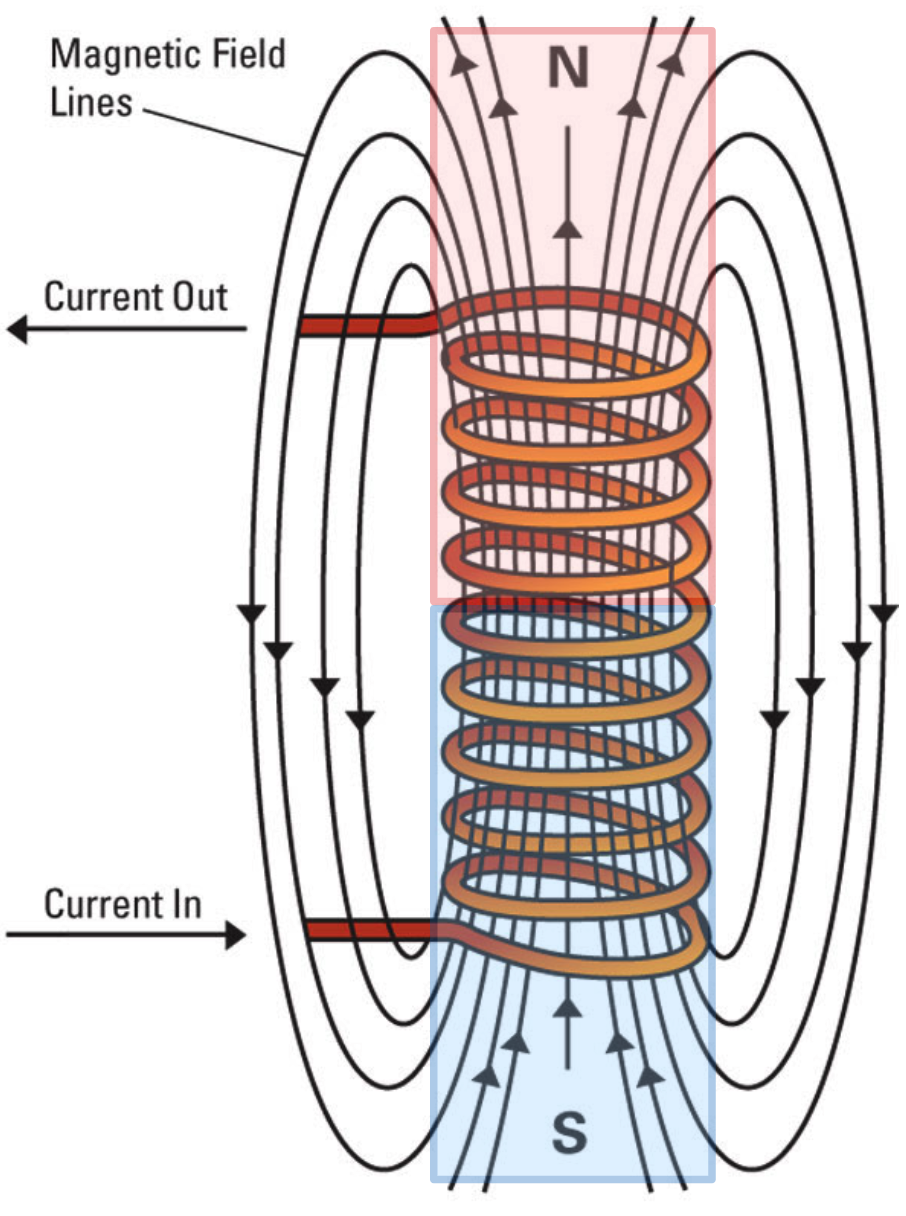
\includegraphics[width=6cm]{FigurasMemoria/electromagnet.png}
    \caption{Visualización del campo magnético de una bobina energizada.}
    \label{fig:electromagnet2} %Para referenciar -> \ref{fig:figNum}
\end{figure}

Por ende, si a la situación que observamos en la figura anterior, le añadimos un elemento de material ferromagnético en uno de los extremos del solenoide, este se verá atraído hasta su centro. Aprovechando este suceso, podemos controlar la alimentación de la bobina para que solamente esté energizada durante el tiempo necesario para atraer el vástago al punto deseado. Una vez que el vástago alcance el centro de la bobina, cortaremos la alimentación para que deje de ser atraído y continúe su movimiento por inercia. El objetivo final de la práctica es predecir cuál va a ser la fuerza ejercida por la bobina sobre el proyectil mediante software, optimizar la geometría para conseguir la mayor densidad energética posible y comprobar las predicciones en el banco de pruebas.

\subsection*{Modelo de la bobina y parámetros iniciales}

El modelo del sistema con el que trabajaremos durante los siguientes apartados consta de las siguientes variables:

\begin{itemize}
    \item \textbf{Parámetros geométricos}:
    \begin{enumerate}[label=\alph*., leftmargin=*, itemindent=1em]
        \item \(r_{cext}\) y \(r_{cint} \): radios exterior e interior de la bobina, respectivamente [m].
        \item \(l_c\): altura de la bobina [m].
        \item \(D_{cu}\): diámetro de la sección del conductor [m].
        \item \(r_{fe}\): radio del vástago [m].
        \item \(l_{fe}\): longitud del vástago [m].
        \item \(k_{disp}\): parámetro multiplicador para obtener la sección de dispersión.
    \end{enumerate}
    \item \textbf{Parámetros eléctricos}:
    \begin{enumerate}[label=\alph*., leftmargin=*, itemindent=1em]
        \item \(N\): número de espiras.
        \item \(I_{cc}\): corriente de alimentación del solenoide [A].
        \item \(\mu_0 = 4\pi*10^{-7}\): permeabilidad del vacío [Hm\(^{-1}\)]. 
        \item \(\mu_{fe}\): permeabilidad relativa del vástago ferromagnético.
    \end{enumerate}
\end{itemize}

\begin{figure}[H]
    \centering 
    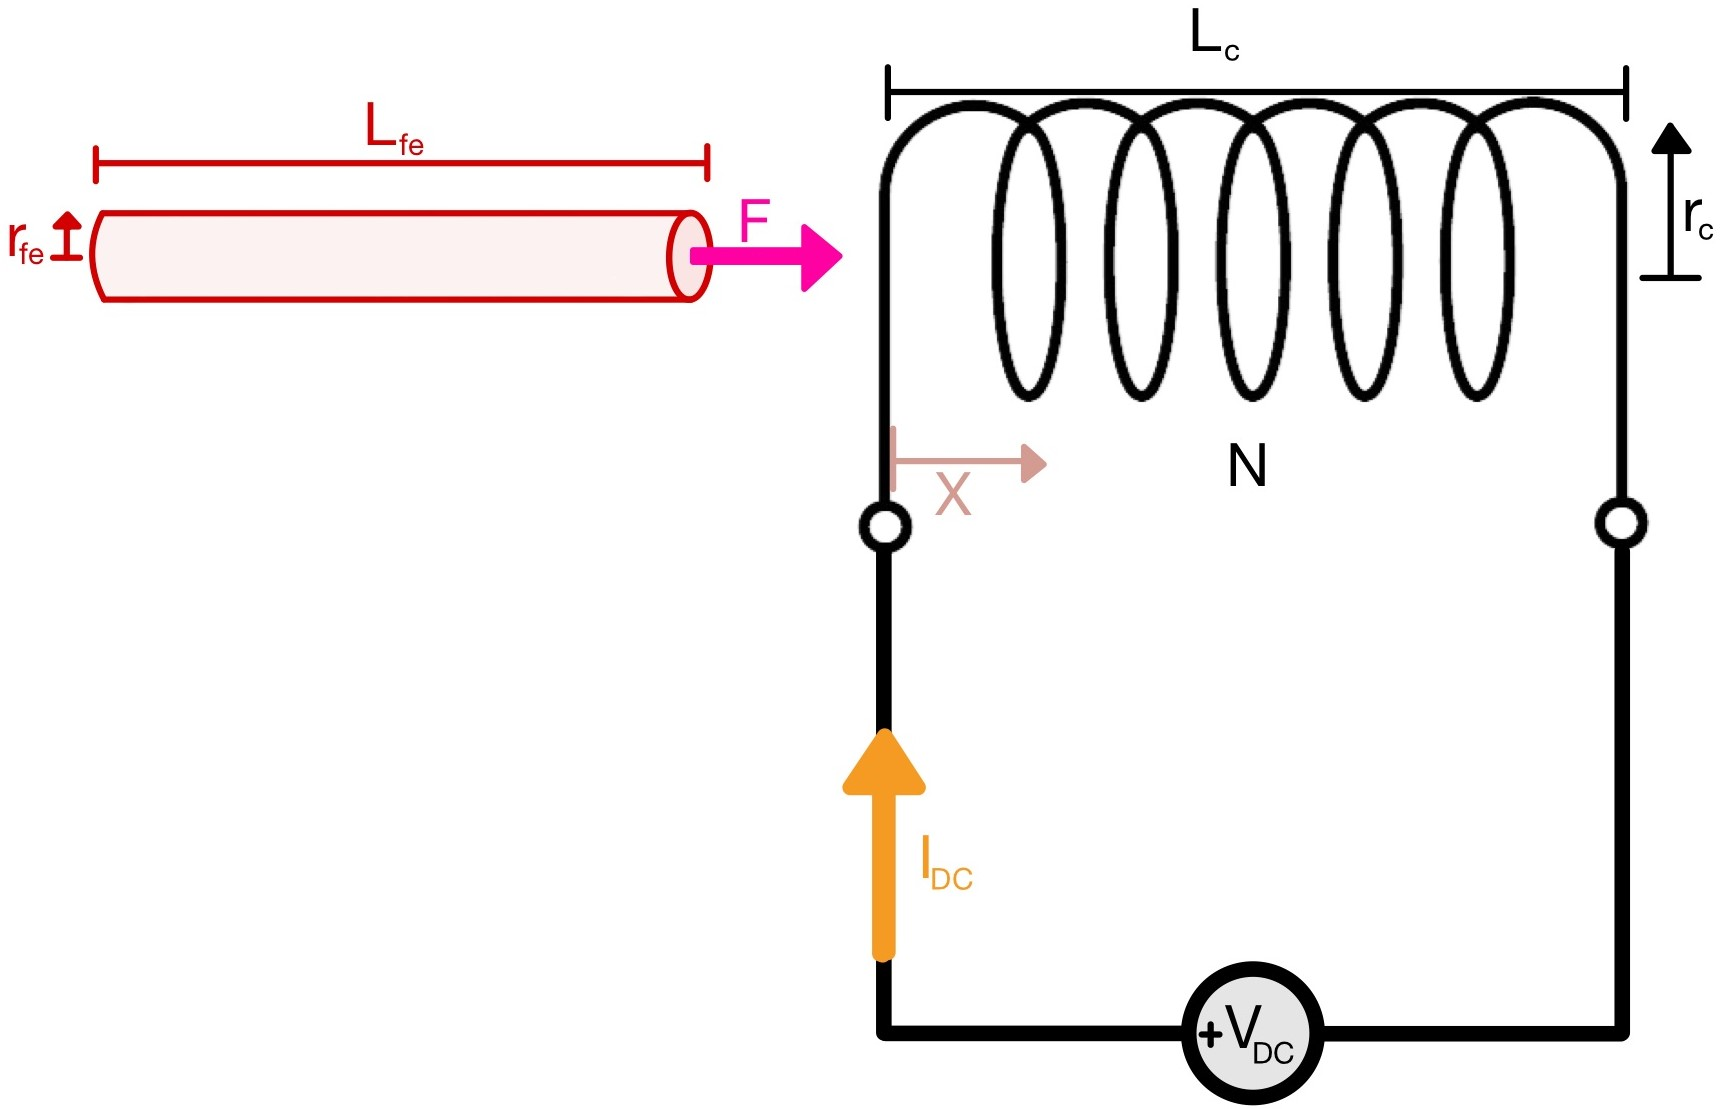
\includegraphics[width=10cm]{FigurasMemoria/esquemaDesTeor.jpg}
    \caption{Esquema geométrico del sistema.}
    \label{fig:esquemaGeomPractica} %Para referenciar -> \ref{fig:figNum}
\end{figure}

El primer paso de esta práctica será elegir la geometría de la bobina inicial sobre la que se realizarán los cálculos de los modelos y las pruebas iniciales. Para ello, se debe rellenar la tabla \ref{tab:bobIniPractica} con valores dentro de los intervalos especificados y teniendo en cuenta las siguientes condiciones:

\begin{itemize}
    \item \(r_{cext} = r_{cint} + \frac{ND_{cu}^2}{l_c}\)
    \item \(r_{cext} \leq XXX\)
    \item \(l_c \leq XXX\)
    \item \(l_c \leq l_{fe}\)
    \item El valor de \(r_{cint}\) dependerá del cilindro sobre el que se vaya a bobinar el solenoide. Elegirlo del laboratorio y tomar la medida. \textbf{O HABLO CON JOSE A VER QUE TIENE EN EL LAB Y LO DEJAMOS FIJO}
\end{itemize}

\begin{table}[H]
    \centering
    \setlength{\tabcolsep}{5pt}
    \renewcommand{\arraystretch}{1.2}
    \begin{tabular}{|c|c|c|c|c|c|c|}
        \hline
        \hbox{} & \textbf{\(D_{cu}\) [m]} & \textbf{\(r_{cint}\) [m]} & \textbf{\(l_c\) [m]} & \textbf{\(r_{fe}\) [m]} & \textbf{\(l_{fe}\) [m]} & \textbf{N} \\
        \hline
        \textbf{Valor mínimo} & XX & XX & 0.5 & XX & XX & 1 \\
        \textbf{Valor máximo} & XX & XX & XX & XX & XX & - \\
        \hline
        \textbf{Valor elegido} &  &  &  &  &  &  \\
        \hline
    \end{tabular}
    \caption{Valores iniciales para la bobina de la lanzadera.}
    \label{tab:bobIniPractica}
\end{table}


\subsection*{Modelo analítico en MatLAB}

El objetivo de esta parte es computar el modelo de la figura \ref{fig:esquemaGeomPractica} en MatLAB para que devuelva unas gráficas con la evolución de la fuerza de atracción experimentada por el vástago en función de su posición.

Para ello, será necesario realizar el circuito magnético equivalente del sistema. Dicho circuito estará compuesto por las siguientes reluctancias, que deben ser desarrolladas por el alumno:

\[\mathcal{R} = \frac{l_{caract}}{\mu_r\mu_0 S_{efect}}\]

\begin{itemize}
    \item \(\mathcal{R}_{disp~c}\): Será la reluctancia de dispersión de la bobina. No es dependiente de \textit{x}.
    \item \(\mathcal{R}_{Fe}\): Será la reluctancia correspondiente al vástago. No es dependiente de \textit{x}.
    \item \(\mathcal{R}_{\phi}\): Será la reluctancia correspondiente al camino del flujo magnético que abraza todo el sistema. Es dependiente de \textit{x}.
    \item \(\mathcal{R}_{aire~c}\): Será la reluctancia correspondiente al volumen de aire que hay dentro de la bobina. Es dependiente de \textit{x}.
\end{itemize}

Una vez elegidas las longitudes y secciones efectivas de cada una de las reluctancias expresadas, se podrá calcular la inducción magnética según:

\[B = \frac{NI}{\sum\mathcal{R}}\]

Y la expresión de la fuerza de atracción magnética sobre un cuerpo \textit{T} cualquiera es:

\[F_T = \frac{1}{2} \frac{B_T^2*S_{efect~T}}{\mu_0}\]

Teniendo en cuenta que \textit{x} es la posición del extremo del vástago, que su intervalo de interés para la práctica es \(x\in [0, l_c]\) y que el circuito magnético cambia para cada valor de \textit{x}, se pide diseñar el código y rellenar las figuras \ref{fig:grafReluctPractica}, \ref{fig:grafInducPractica} y \ref{fig:grafFuerzaPractica} con los los valores obtenidos. El resultado puede ser algo como:

\begin{figure}[H]
    \centering 
    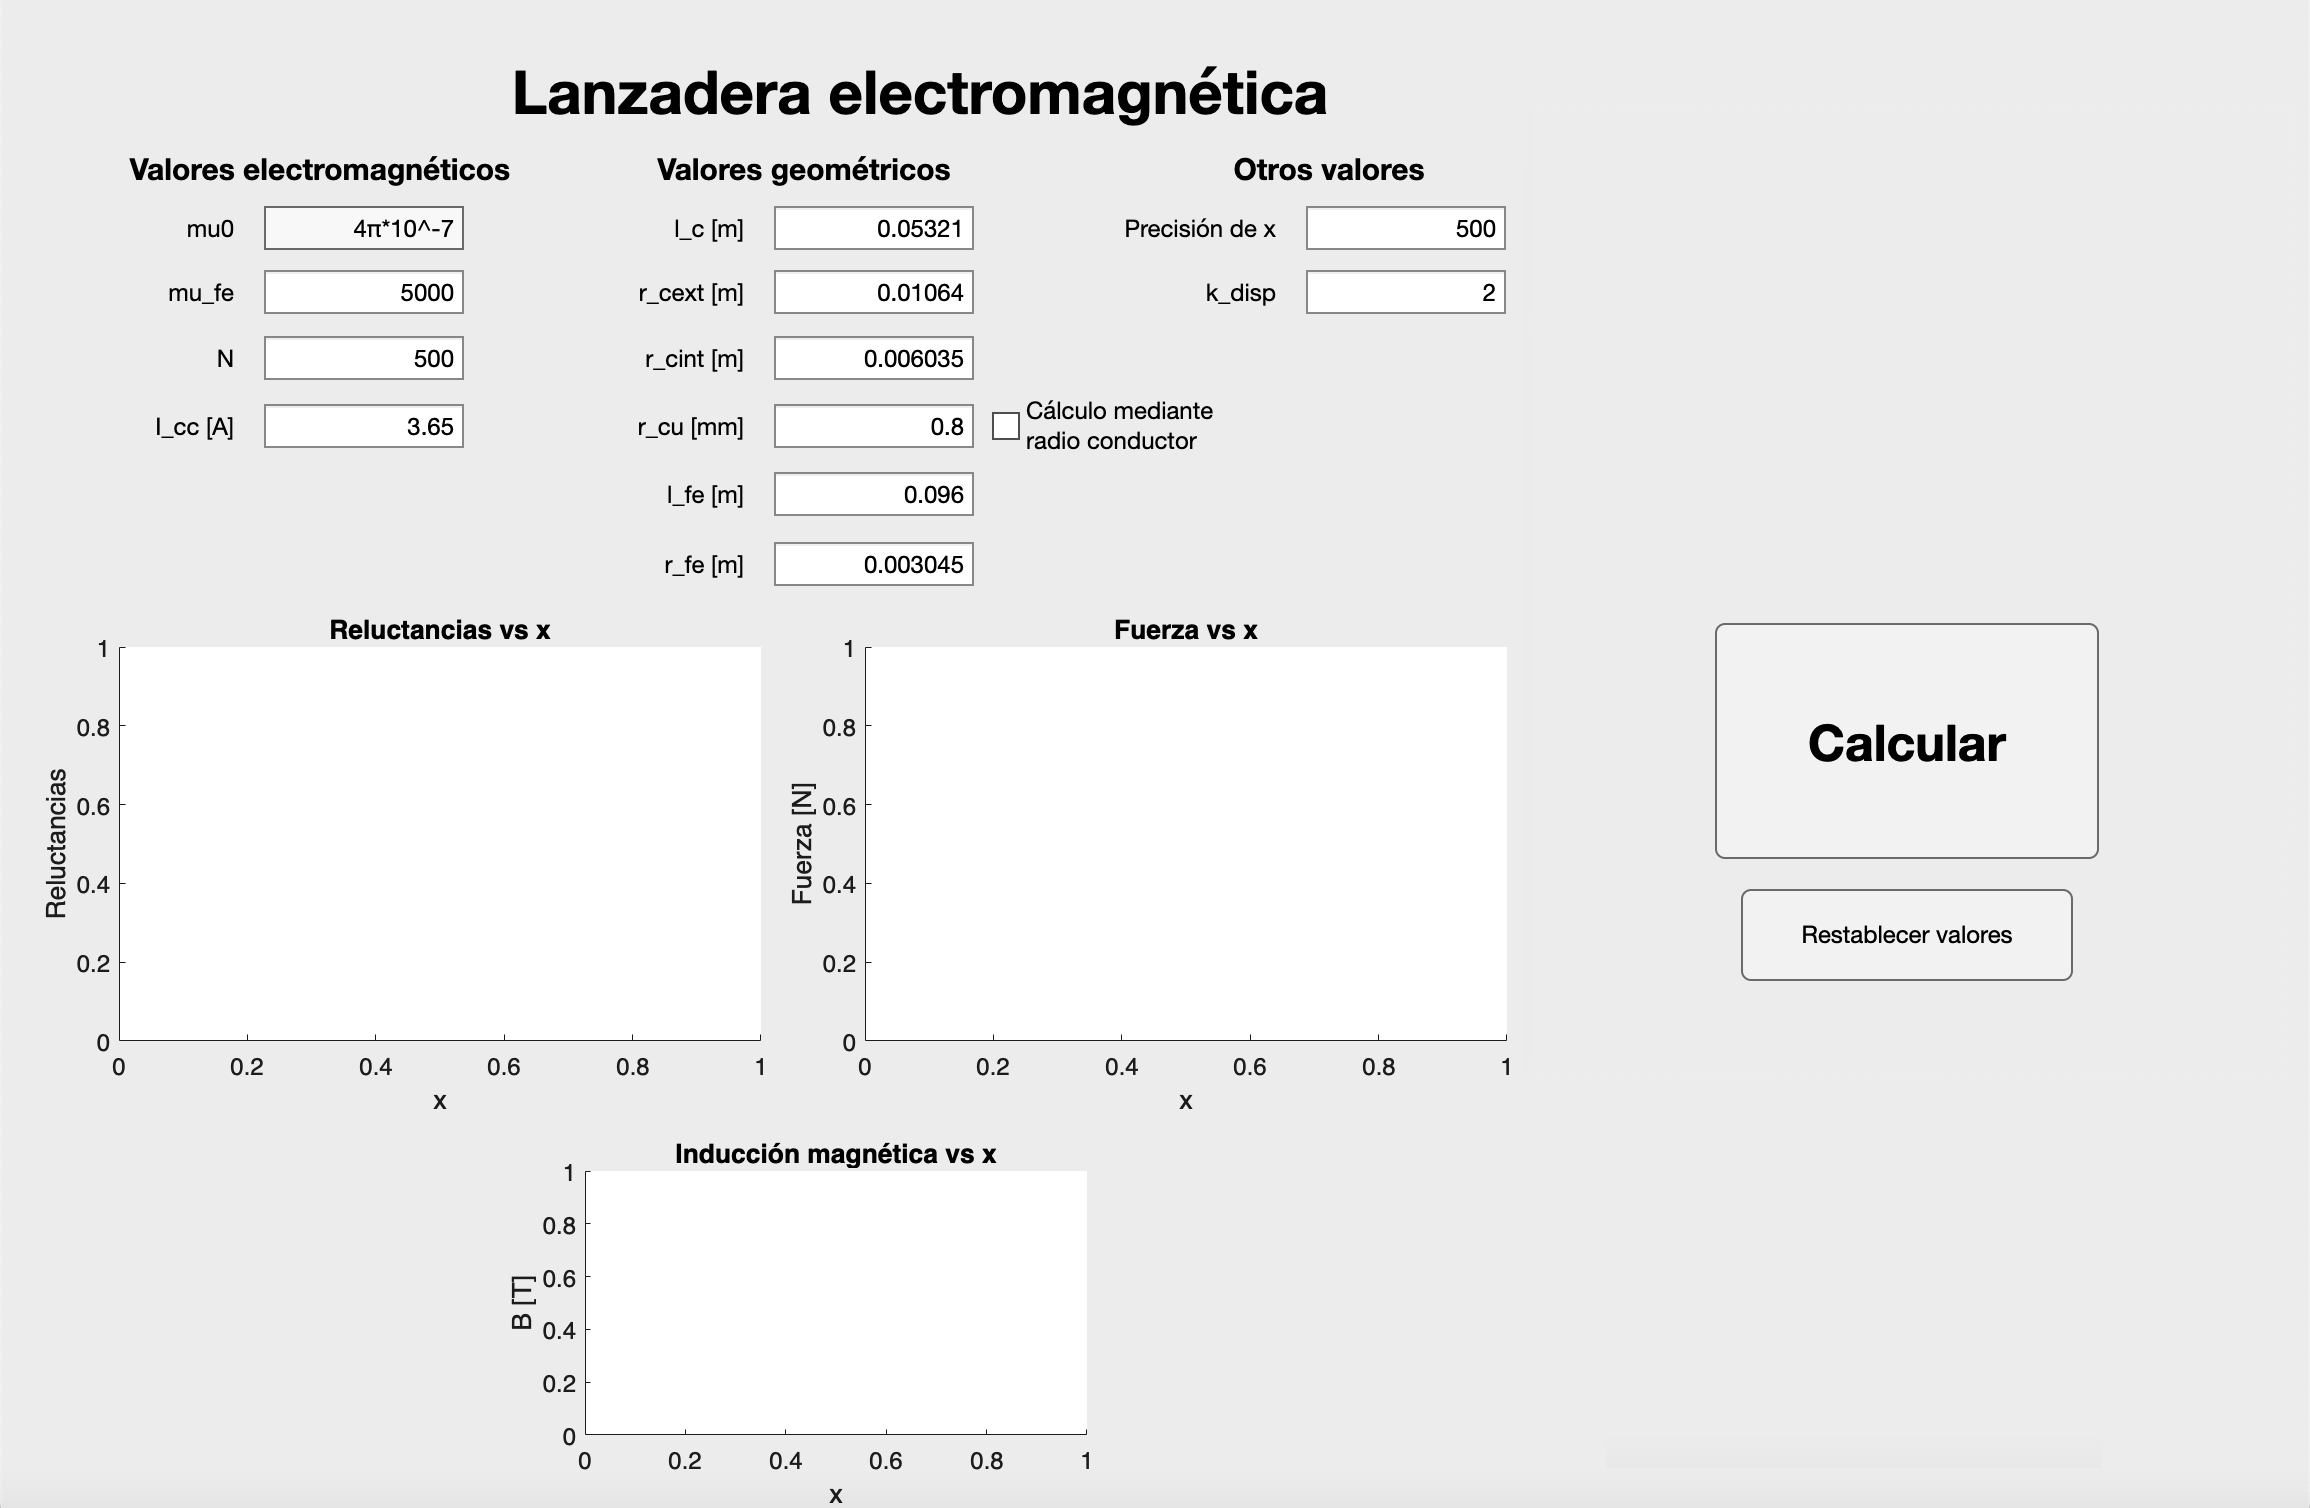
\includegraphics[width=7cm]{FigurasMemoria/calculadoraSinPista.png}
    \caption{Aplicación de ejemplo.}
    \label{fig:calculadoraSinPista} %Para referenciar -> \ref{fig:figNum}
\end{figure}

\newpage

\begin{figure}[H]
    \centering 
    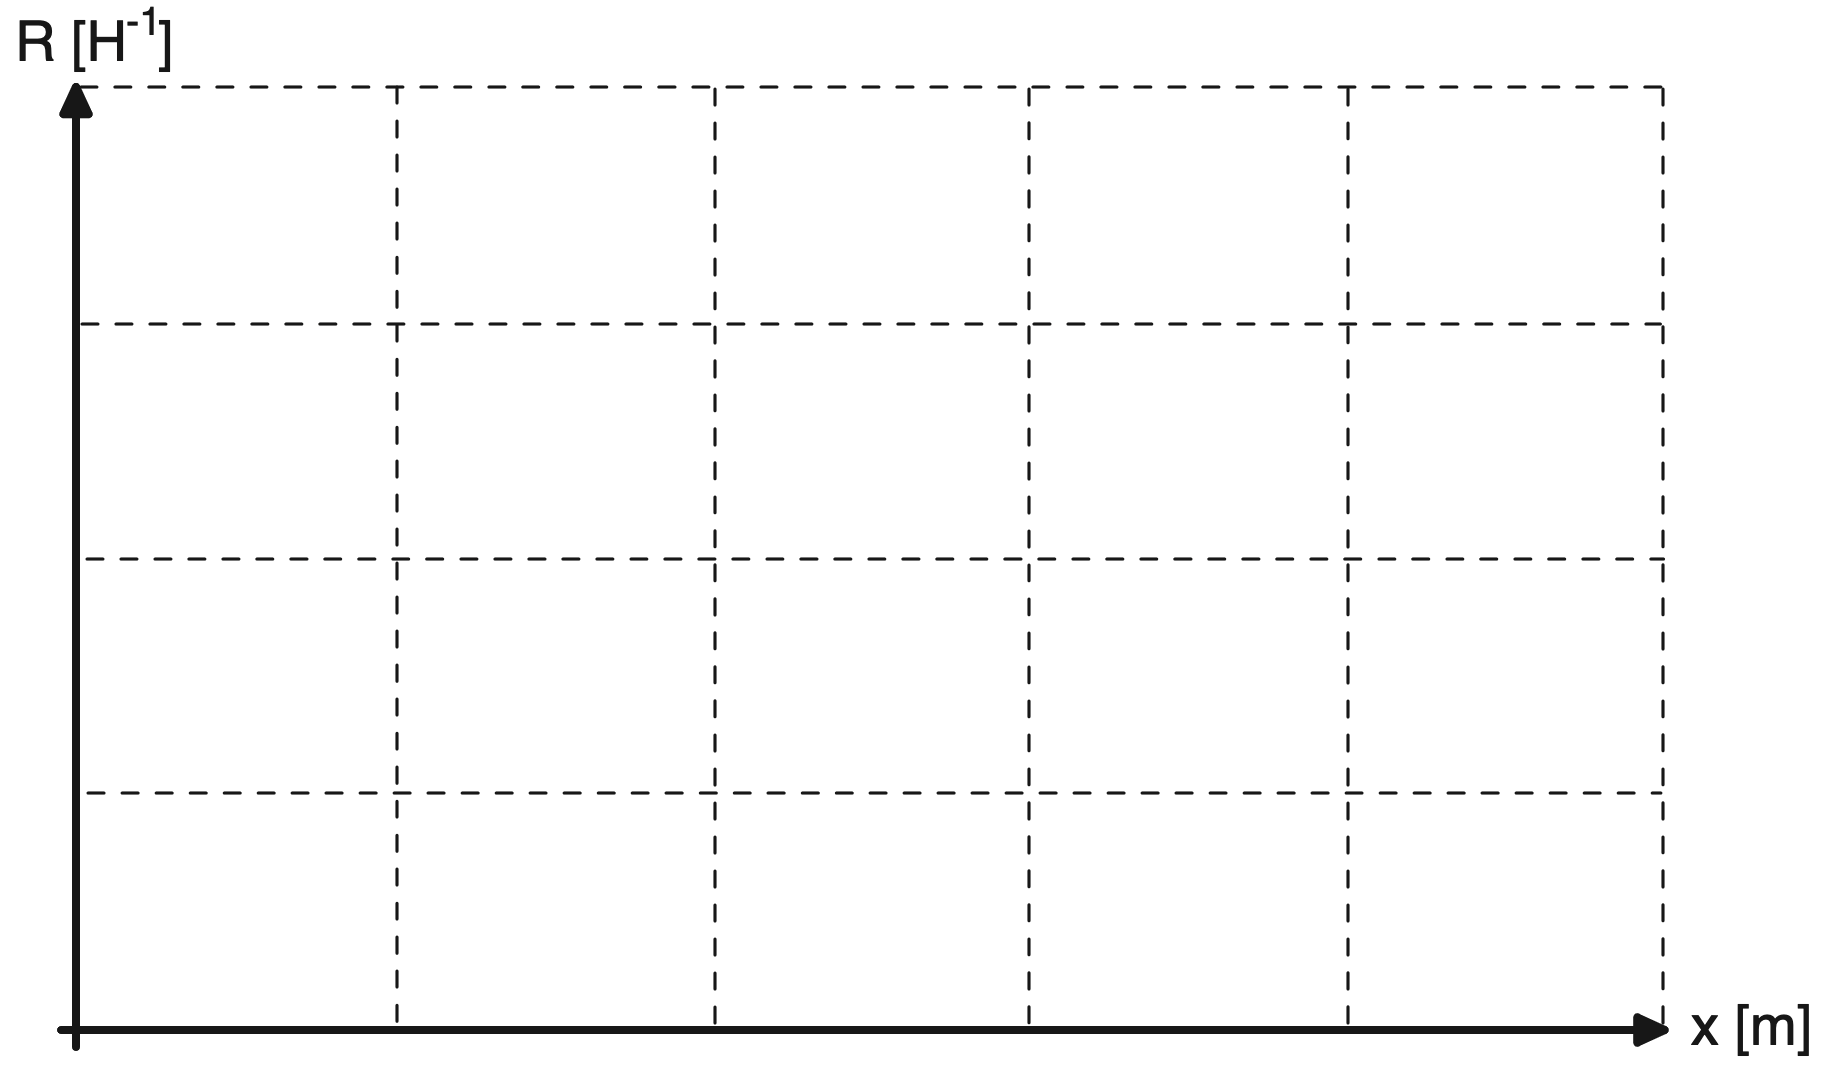
\includegraphics[width=0.75\textwidth]{FigurasMemoria/grafReluctPractica.png}
    \caption{Reluctancia en función de \textit{x}.}
    \label{fig:grafReluctPractica} %Para referenciar -> \ref{fig:figNum}
\end{figure}

\begin{figure}[H]
    \centering 
    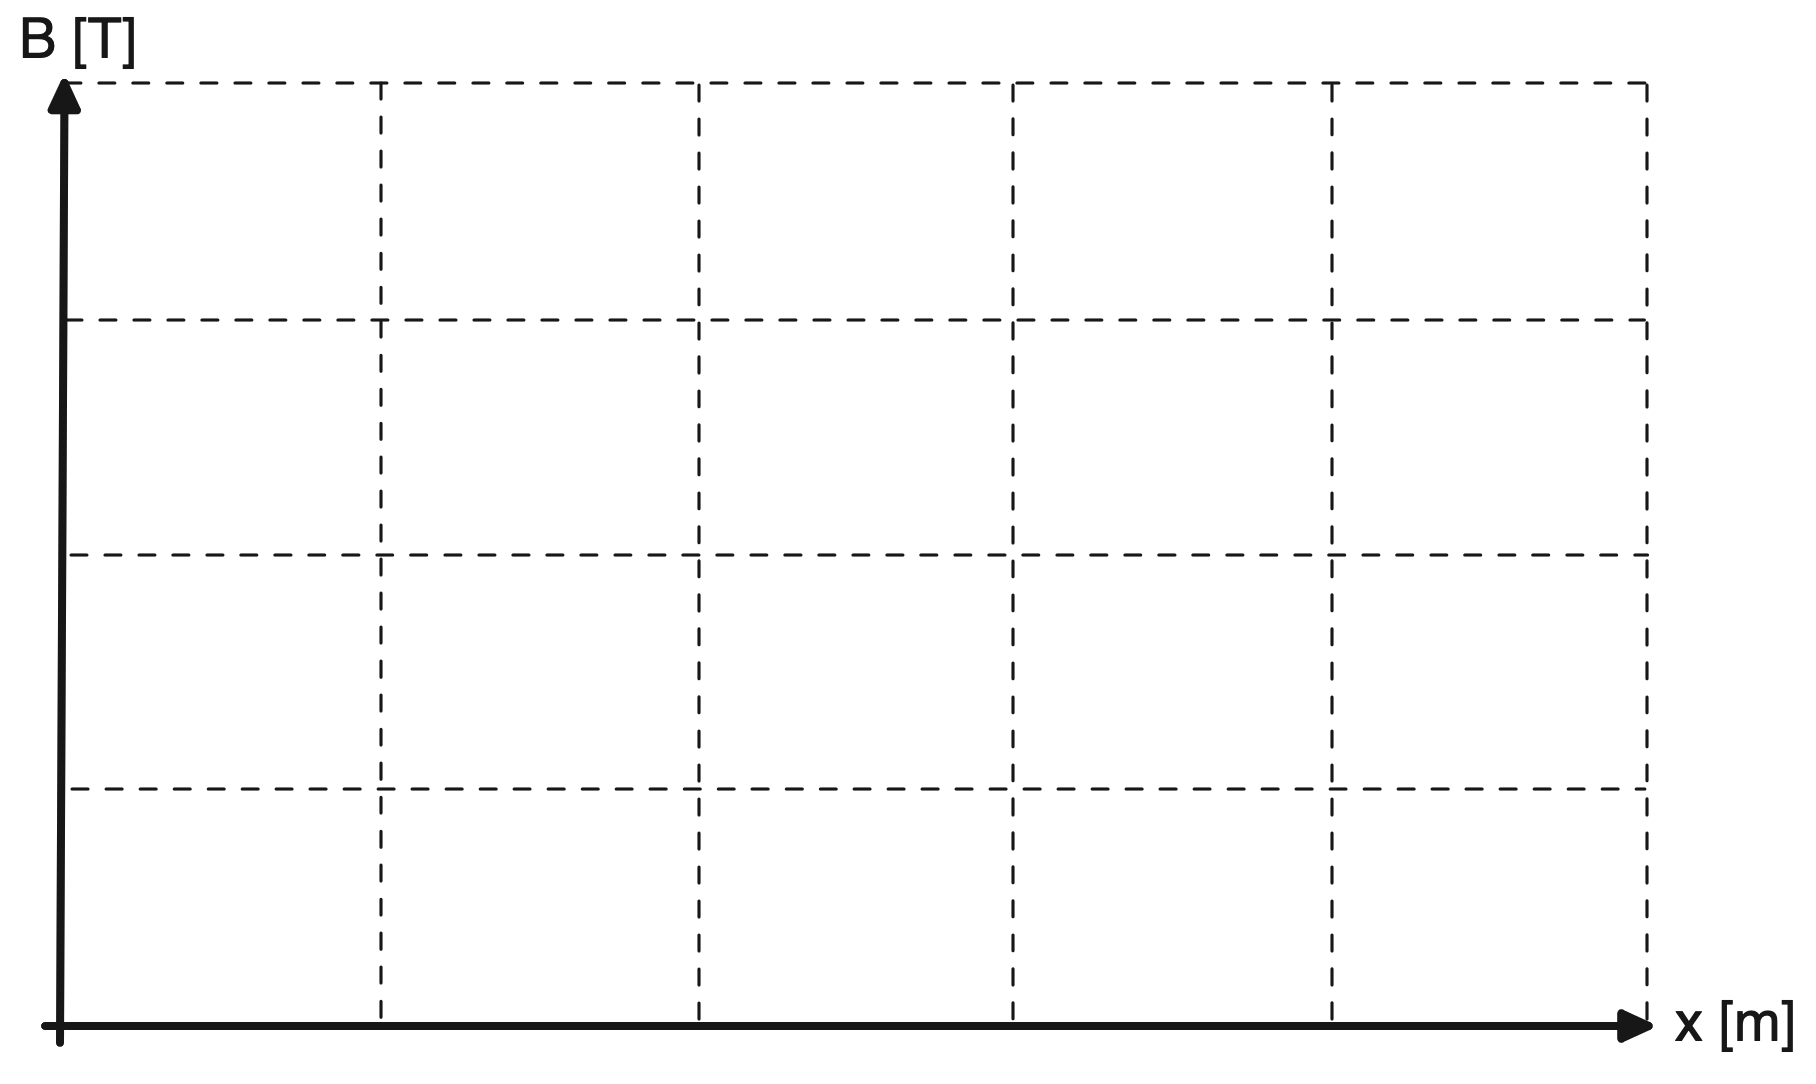
\includegraphics[width=0.75\textwidth]{FigurasMemoria/grafInducPractica.png}
    \caption{Inducción magnética en función de \textit{x}.}
    \label{fig:grafInducPractica} %Para referenciar -> \ref{fig:figNum}
\end{figure}

\begin{figure}[H]
    \centering 
    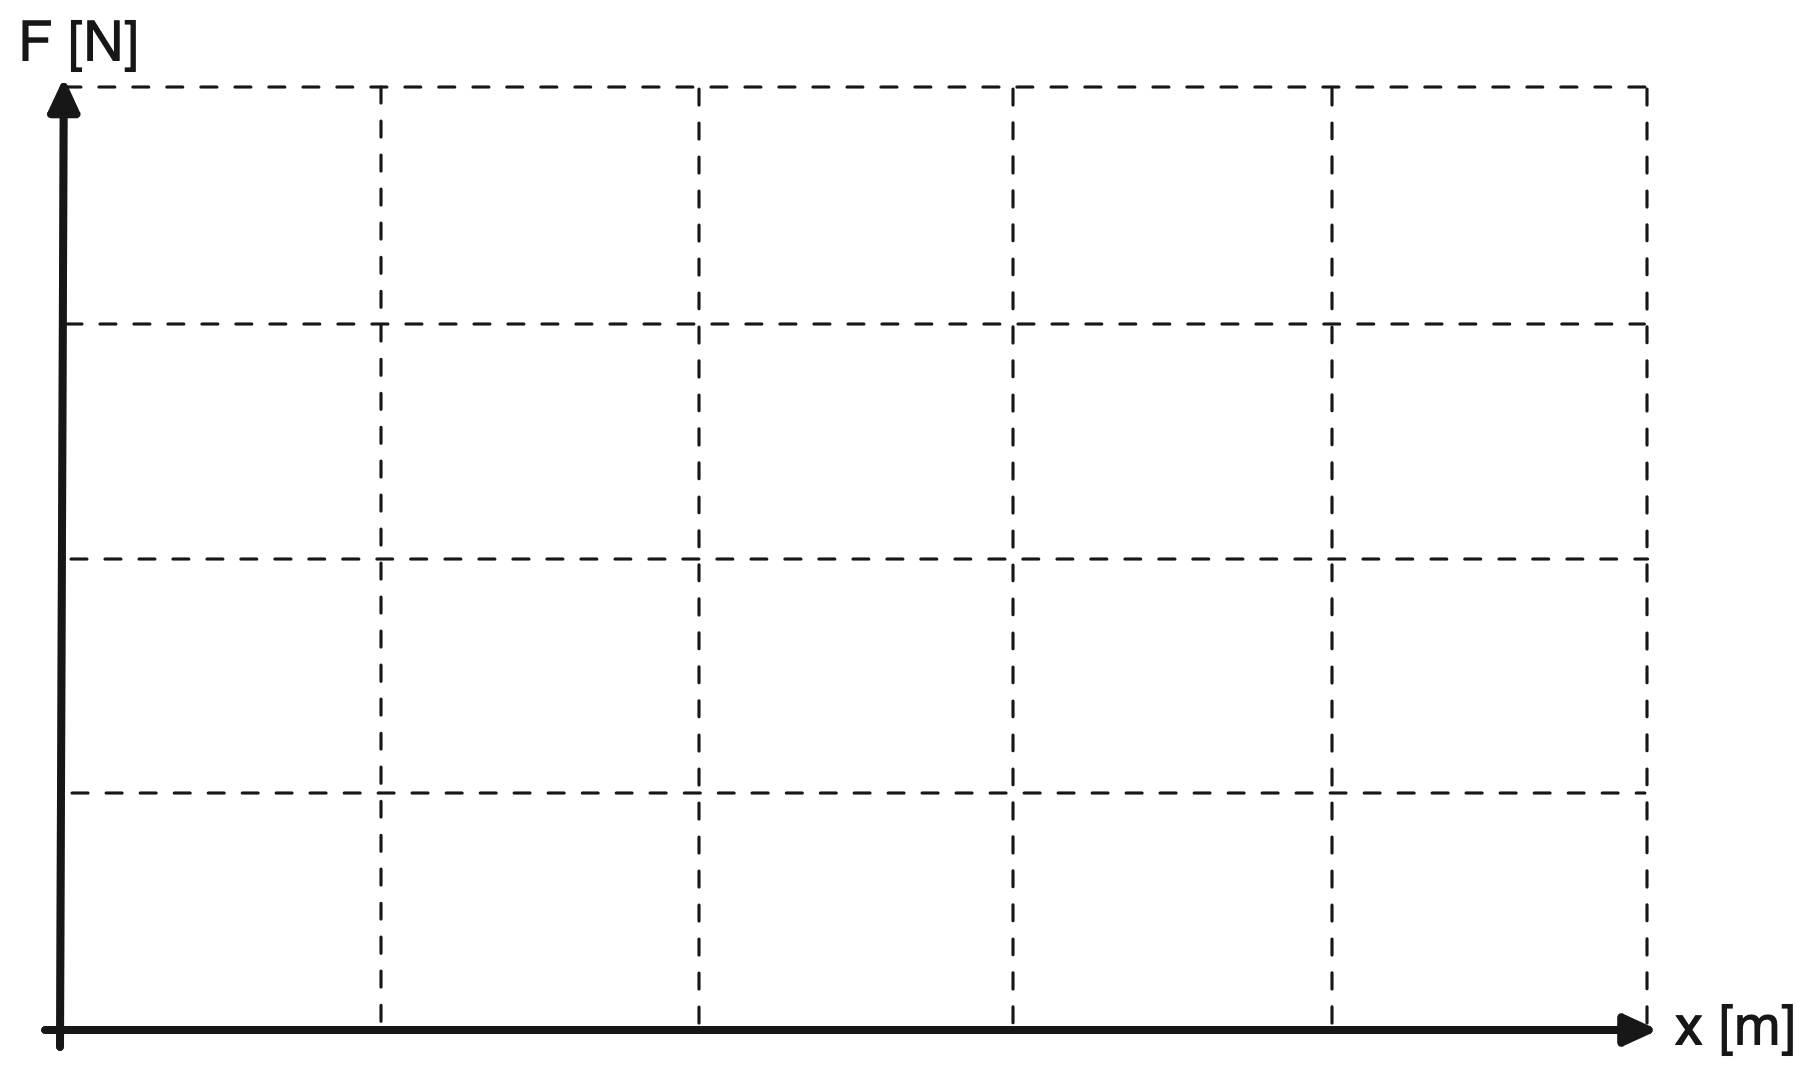
\includegraphics[width=0.75\textwidth]{FigurasMemoria/grafFuerzaPractica.png}
    \caption{Fuerza de atracción magnética en función de \textit{x}.}
    \label{fig:grafFuerzaPractica} %Para referenciar -> \ref{fig:figNum}
\end{figure}

\subsection*{Modelo de elementos finitos en ANSYS Maxwell}

\textbf{ESTA SECCIÓN NO SE SI INCLUIRLA EN LA PRÁCTICA DE LOS ALUMNOS, PERO LA DESCRIBO POR SI TE PARECE QUE ESTÁ BIEN}

El software ANSYS Maxwell o ANSYS Electronics, es una rama del software de simulación por elementos finitos ANSYS, utilizado para realizar simulaciones electromagnéticas tanto instantáneas como transitorias. Este apartado de la práctica consistirá en definir la geometría de la tabla \ref{tab:bobIniPractica} en ANSYS para conseguir dos objetivos: visualizar los campos magnéticos y obtener un valor para la fuerza de atracción. Como este es un software con el que el alumno no está familiarizado, se presenta a continuación una guía para poder realizar esta parte de la práctica:

\subsubsection*{Creación del proyecto}

El primer paso será abrir ANSYS Maxwell e inicializar el proyecto. Para ello, pulsaremos la tecla de menú de inicio (\faWindows{}) y escribiremos ``ANSYS Maxwell''. Pulsaremos aceptar en las ventanas que aparezcan hasta que salga lo siguiente:

\textbf{IMAGEN DE INICIO AM}

Ahora abriremos un nuevo proyecto en 3D clicando en la siguiente parte del menú:

\textbf{IMAGEN/ES DE CREACIÓN DE PROYECTO 3D}

El siguiente paso será empezar a definir la geometría. Esto hará de manera paramétrica, es decir, asignando a variables las medidas de los polígonos que utilicemos, lo que nos permitirá cambiar de solenoide fácilmente o realizar pruebas en distintos dispositivos que montemos en el laboratorio. Las variables o parámetros serán los mismos que los expuestos en el apartado de "Modelo de la bobina y geometría inicial". Para incluir estos parámetros, nos dirigiremos al menú de "Variables", localizado en la ventana de abajo a la izquierda. Las variables se añaden de la siguiente manera:

\textbf{IMAGEN DE ADICIÓN DE PARÁMETROS DEL SISTEMA}

En ANSYS Maxwell, hay dos maneras de representar una bobina. Para inductores electrónicos, que generalmente tienen pocas espiras y una trayectoria muy definida, se puede crear una función helicoidal que represente la bobina de manera fidedigna a la realidad, pero se convierte en algo imposible cuando se trata de una bobina en el orden de magnitud en el que trabajaremos en esta práctica, pues hay muchas capas de conductores que no son uniformes, con radios diferentes entre capa y capa y número de conductores distinto, lo que convierte la tarea de describir la función en algo innecesariamente difícil. En cambio, ANSYS permite generar un cilindro, especificar unos terminales, una resistencia y un número de espiras para tratarlo como un solenoide con los conductores distribuidos de manera homogénea en su volumen. Esto es muy conveniente, ya que simplifica el proceso a los siguientes pasos:

\textbf{IMAGENÉS DE COMO GENERAR EL CILINDRO BOBINA} (fig:cilindroAnsys)

Una vez generado el cilindro que representa la bobina, el siguiente paso es generar otro cilindro de manera análoga en el centro del primero, que se corresponderá con el vástago. Lo único que debemos de tener en cuenta a la hora de definir el vástago, es que es útil definir su posición en función de la altura de la bobina, para que después podamos ver con facilidad la evolución de los campos en función de la posición. También será necesario hacer clic izquierdo sobre la geometría seleccionada y añadirle el parámetro de fuerza. A continuación se muestran unas imágenes que explican el proceso de creación del vástago:

\textbf{IMÁGENES DE COMO GENERAR EL CILINDRO VÁSTAGO}

El siguiente paso es añadir las cualidades de bobina al cilindro de la figura %\ref{fig:cilindroAnsys}
para lo cual tendremos que realizar una sección en uno de los planos verticales, la cual se corresponderá con uno de los terminales de la bobina... \textbf{TERMINAR LA EXPLICACIÓN NO ME ACUERDO DE CABEZA}

\textbf{IMÁGENES DE CREACIÓN DE TERMINALES}

El siguiente paso necesario es definir una región de aire para poder dar las condiciones de contorno al sistema. Para ello pulsaremos el botón de \textit{region} en el menú del modelo, y definiremos un cubo con un 500\% de offset partiendo del origen de coordenadas. Luego seleccionaremos sus bordes y le asignaremos la condición de contorno de \textit{insulating}.

\textbf{IMÁGENES DE CREACIÓN DE LA REGION}

Para simular el comportamiento del sistema correctamente, será necesario definir también los materiales de cada una de las geometrías que hemos definido. Para ello, seleccionamos la geometría y buscamos su material, el cual será \textit{annealed copper} para la bobina y \textit{Steel ENG 100GJL} para el vástago.

\textbf{IMÁGENES DE SELECCIÓN DE MATERIAL}

Para poder obtener la visualización del flujo electromagnético a través del aire, tendremos que añadir un eje de coordenadas relativo al la sección del extremo superior de la bobina para poder dibujar un cuadrado que seccione al solenoide y a la barra por la mitad. Es importante definir este cuadrado como \textit{non-model}, para que no interfiera con las interacciones electromagnéticas del modelo. 

\textbf{IMÁGENES DE GENERACIÓN DEL CUADRADO DE VISUALIZACIÓN}


Por último antes de empezar a simular, debemos definir el tipo de solución que estamos buscando. Para ello, pulsaremos el apartado de \textit{Setup} con el botón izquierdo del ratón... \textbf{TERMINAR CON ANSYS DELANTE}

\textbf{IMÁGENES DE CREACIÓN DEL SETUP}

Con este último paso, debería estar todo listo para realizar la primera simulación. De todas formas, para comprobarlo, iremos al apartado de \textit{Simulation} y pulsaremos el tick verde que dice \textit{Verify}. Si todo sale en verde, podemos pulsar \textit{Analyze All} y ANSYS empezará a ejecutar la simulación, lo cual sabremos por la aparición de una barra verde en la esquina inferior derecha de la pantalla que indica el progreso. Cuando termine, tendremos que ir al apartado de \textit{Solution}, y buscar \textbf{NO RECUERDO EL NOMBRE DEL BOTÓN} para obtener el valor de fuerza de atracción que ANSYS ha calculado para la posición simulada. También podremos obtener la forma del campo magnético si seleccionamos el cuadrado que secciona la geometría, pulsamos el botón derecho del ratón, y navegamos por el menú que aparece siguiendo la ruta \(\text{Fields} \rightarrow B \rightarrow \text{B vector}\).

Una vez explicado el proceso de cómo realizar las simulaciones, se pide que se modifique el valor de la posición del vástago imitando el eje de abscisas de la figura \ref{fig:grafFuerzaPractica} y se rellene la siguiente tabla y gráfica con los diferentes valores del parámetro:

\begin{table}[ht]
    \centering
    \setlength{\tabcolsep}{5pt}
    \renewcommand{\arraystretch}{1.2}
    \begin{tabularx}{\textwidth}{|c|*{12}{>{\centering\arraybackslash}X|}}
        \hline
        \textbf{Fuerza} & \(l_c\) & \(\frac{9}{10} l_c\) & \(\frac{8}{10} l_c\) & \(\frac{7}{10} l_c\) & \(\frac{6}{10} l_c\) & \(\frac{5}{10} l_c\) & \(\frac{4}{10} l_c\) & \(\frac{3}{10} l_c\) & \(\frac{2}{10} l_c\) & \(\frac{1}{10} l_c\) & 0 \\
        \hline
        \(F_x\) &  &  &  &  &  &  &  &  &  &  &  \\
        \(F_y\) &  &  &  &  &  &  &  &  &  &  &  \\
        \(F_z\) &  &  &  &  &  &  &  &  &  &  &  \\
        \(F_{total}\) &  &  &  &  &  &  &  &  &  &  &  \\
        \hline
    \end{tabularx}
    \caption{Valores obtenidos en las simulaciones.}
    \label{tab:simulacionesPractica1}
\end{table}

\begin{figure}[H]
    \centering 
    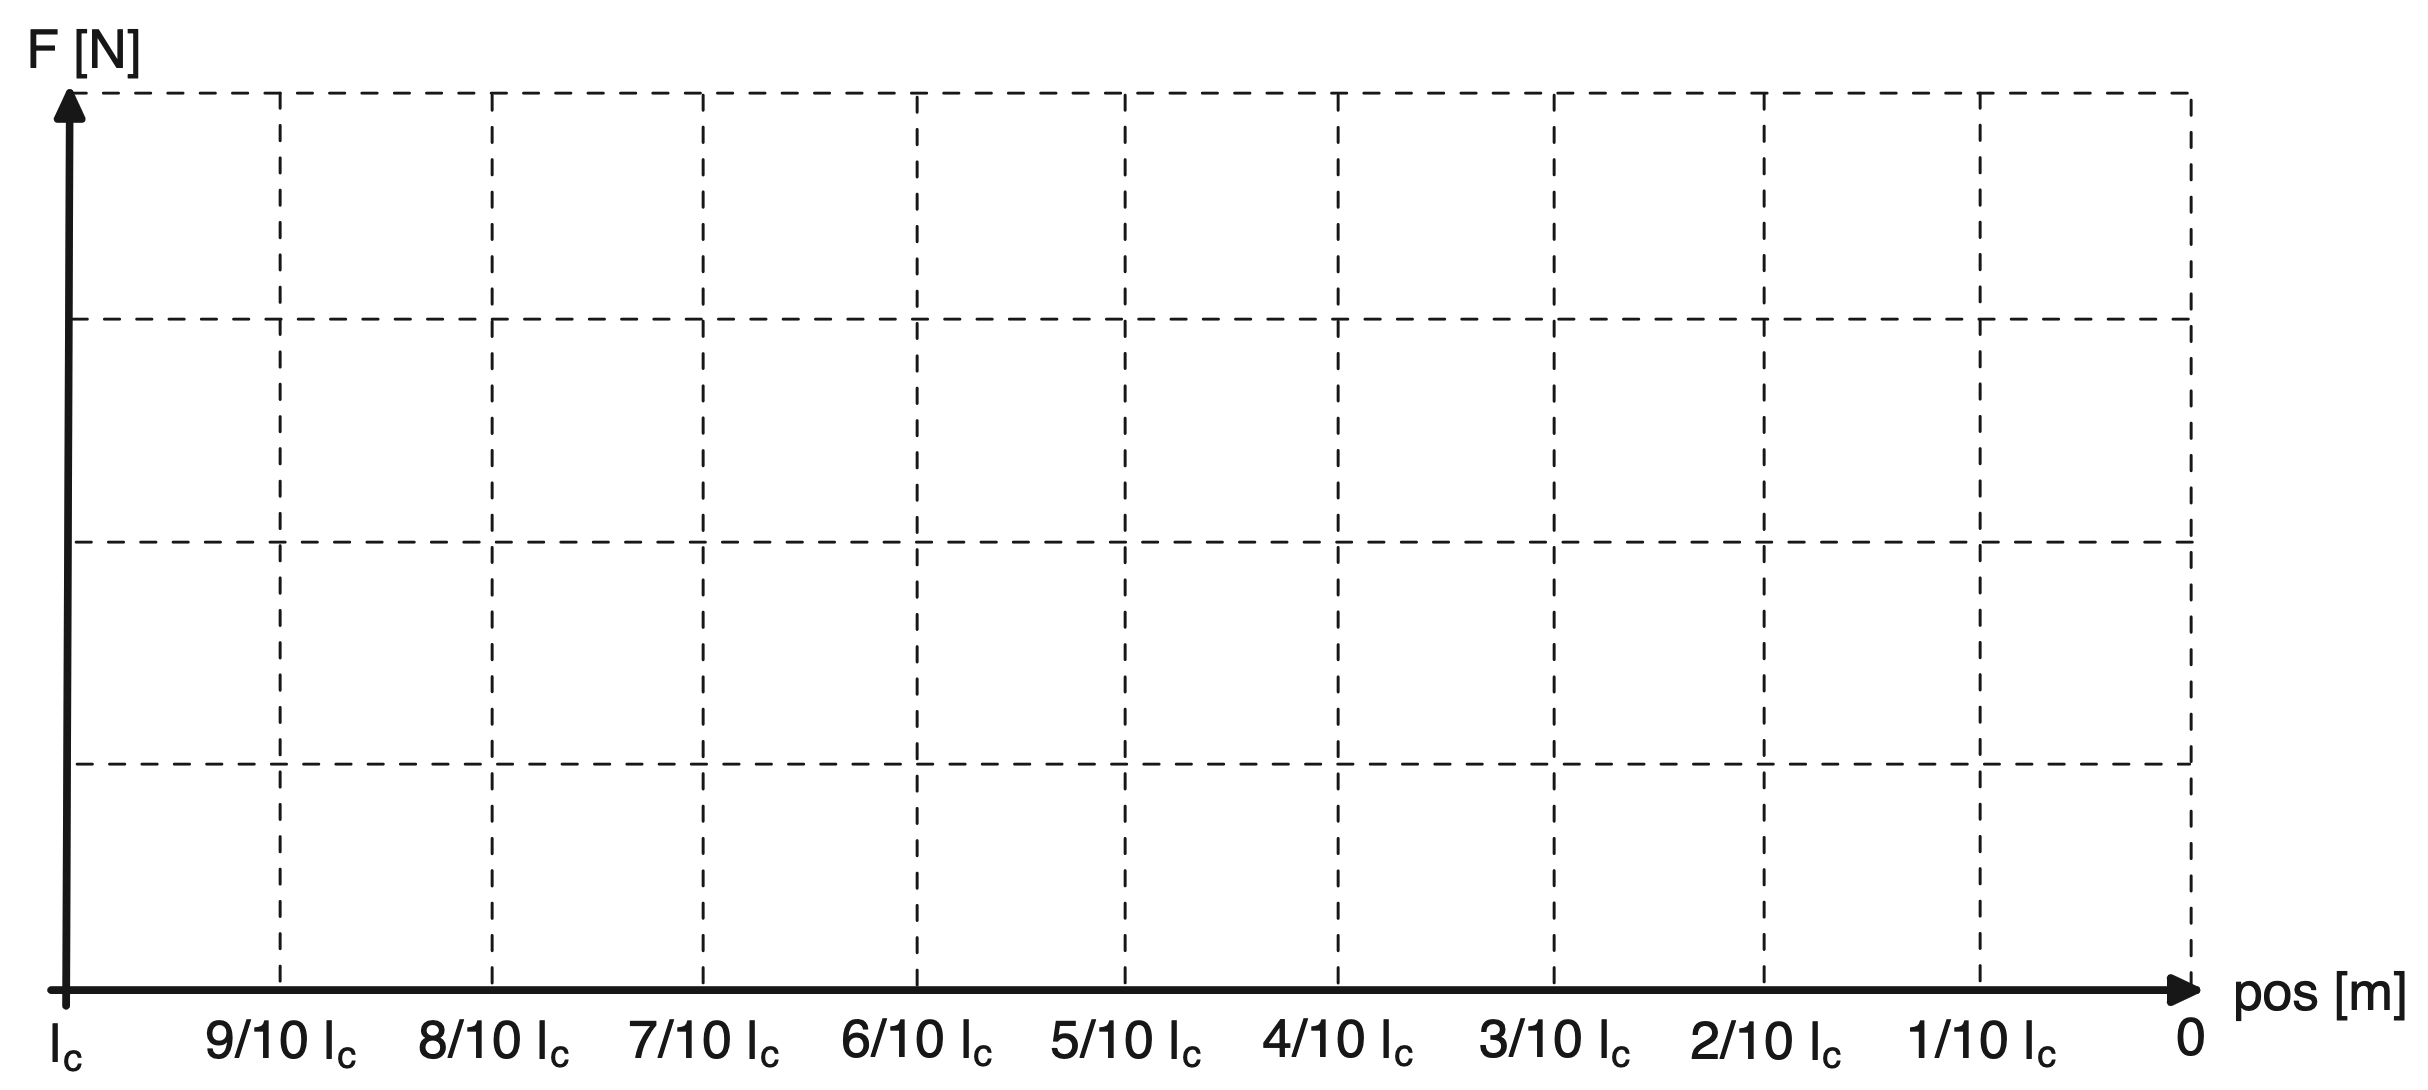
\includegraphics[width=\textwidth]{FigurasMemoria/grafPosAnsysPractica.png}
    \caption{Fuerza de atracción magnética en función de la posición del vástago.}
    \label{fig:grafPosAnsysPractica} %Para referenciar -> \ref{fig:figNum}
\end{figure}

Nótese que los valores de posición varían desde \(l_c\) a 0 debido a que se definen las posiciones de la geometría desde el origen de coordenadas. Esto implica que, en el entorno de ANSYS, \(x_{min} = l_c\) y \(x_{max} = 0\). 

\subsection*{Pruebas en el laboratorio}

En el laboratorio de electricidad se encuentra el \textit{banco de pruebas}, un montaje modular que nos permitirá tomar medidas de la fuerza y velocidad de la bobina.

\begin{figure}[H]
    \centering
    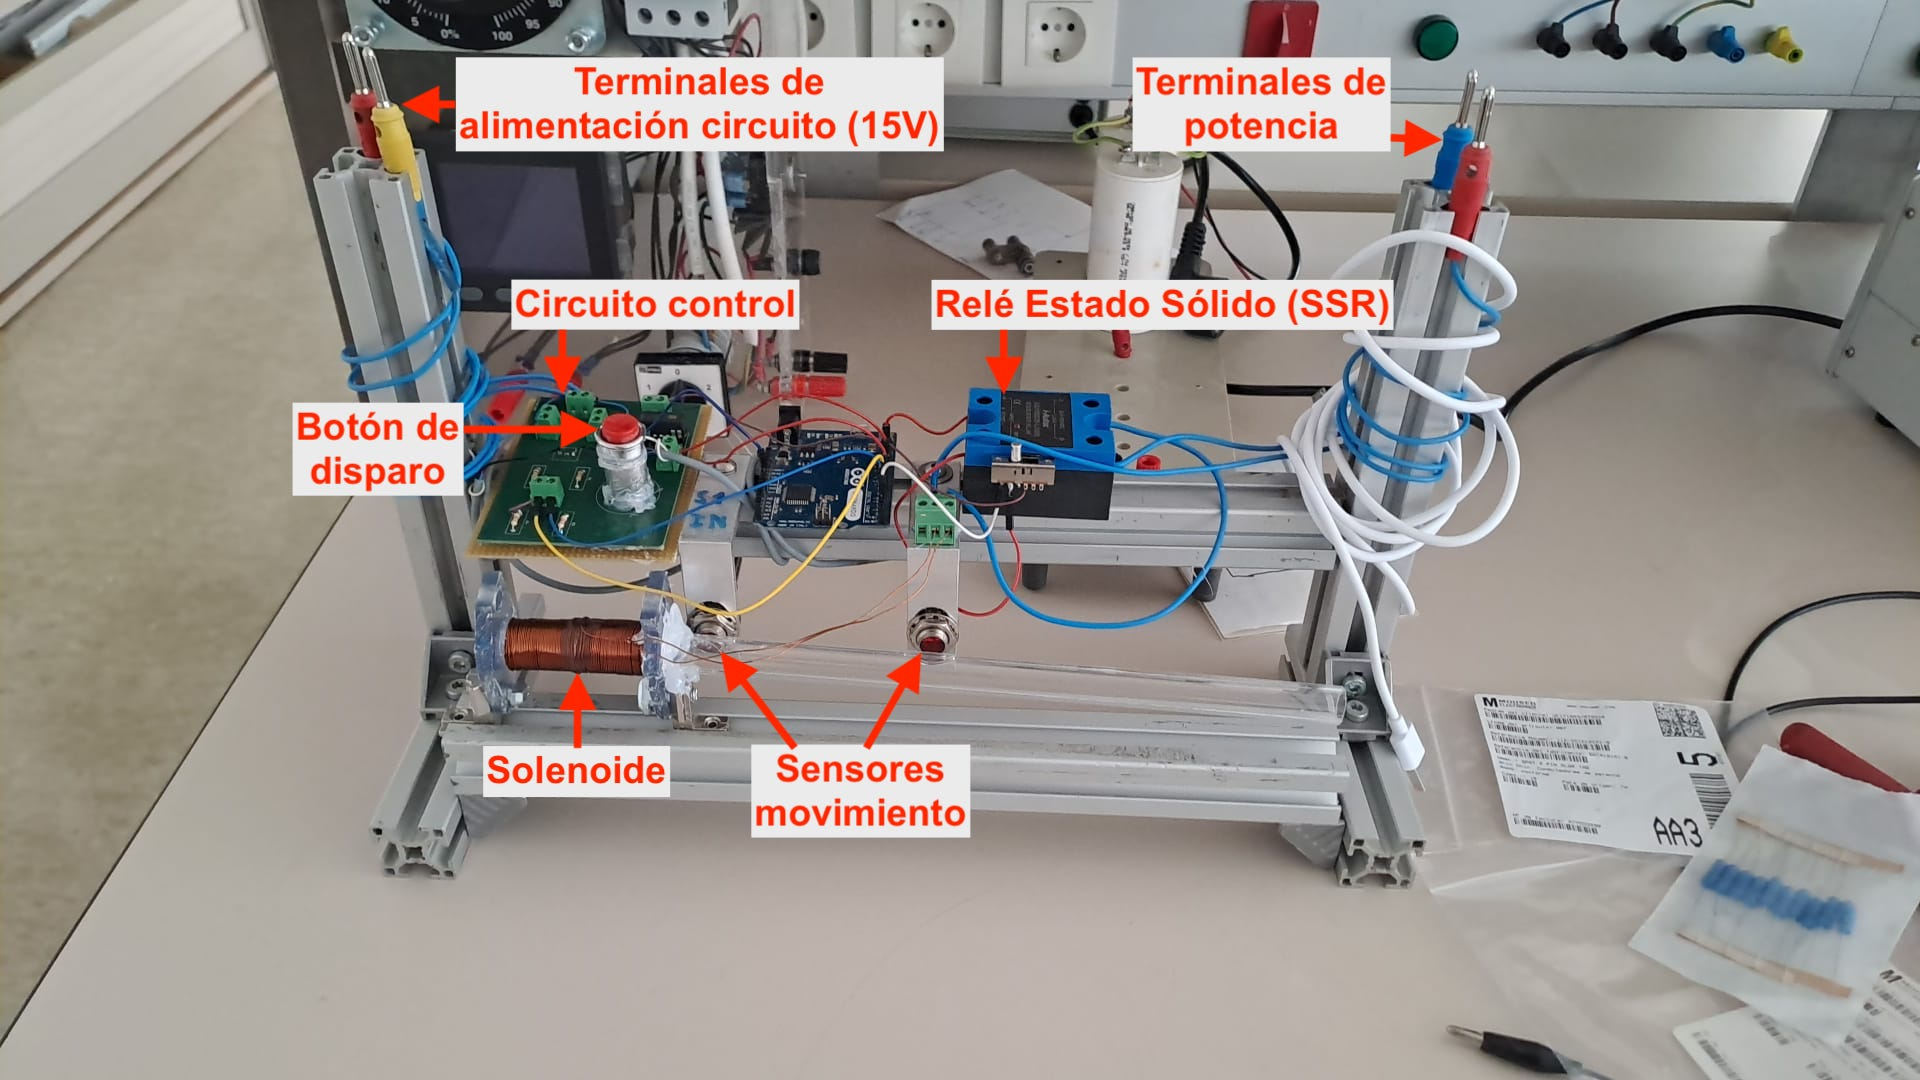
\includegraphics[width=10cm]{FigurasMemoria/prototipoFinalPractica.jpeg}
    \caption{Banco de pruebas.}
    \label{fig:prototipoFinalPractica} %Para referenciar -> \ref{fig:figNum}
\end{figure}

El objetivo esta sección de la práctica es validar los modelos teóricos realizados anteriormente mediante la construcción y prueba de el solenoide de la \ref{tab:bobIniPractica}. Los medios para conseguir esto será emplear montaje de la figura \ref{fig:prototipoFinalPractica}, el cual cuenta con un circuito electrónico que controla los disparos de la bobina así como las mediciones de velocidad del vástago. Las medidas de fuerza se tomarán mediante el uso del dinamómetro.

\textbf{DESPUÉS DE ESCRIBIR TODO ESTO, ME DOY CUENTA DE UNA COSA. ¿CÓMO VAN A SELECCIONAR LA CORRIENTE SI NO TIENEN MANERA DE MEDIR LA RESISTENCIA DE LA BOBINA ANTES DE MONTARLA? YO LO PRIMERO QUE HICÉ FUERON LAS PRUEBAS EXPERIMENTALES, POR LO QUE SABÍA LA CORRIENTE CON LA QUE TRABAJABA. ¿SE LO PONGO ASÍ?}

Para realizar las mediciones de velocidad, habrá que seguir los siguientes pasos:


\begin{enumerate}
    \item Bobinar el solenoide sobre el cilindro escogido en el apartado 1 de la práctica.
    \item Comprobar que el valor \(r_{cext}\) no difiere mucho del calculado analíticamente. Si es así introducir el valor experimental de \(r_{cext}\) en la calculadora.
    \item Acoplar el solenoide al banco de pruebas.
    \item Asegurar que hay un sensor de movimiento justo en la salida del solenoide.
    \item Asegurar que el switch integrado al lado del relé de estado sólido cierra el circuito en el PIN2 del arduino.
    \item Alimentar el sistema:
    \begin{enumerate}
        \item Conectar el circuito eléctronico (terminales de la izquierda) a una tensión de 15 VDC.
        \item Conectar el arduino a un PC o portátil.
        \item Conectar los terminales del relé de estado sólido (terminales de la derecha) a la tensión necesaria para obtener la corriente necesaria.
    \end{enumerate}
    \item Abrir el IDE de arduino.
    \item Subir el programa encontrado en ``URL'' a la placa.
    \item Abrir el \textit{Serial Plotter}.
    \item Colocar el vástago al borde de la bobina.
    \item Pulsar el botón rojo.
    \item Observar la diferencia temporal en el \textit{Serial}.
\end{enumerate}

Una vez obtenida la diferencia temporal, se deberá medir la distancia entre los centros de los sensores para poder completar los cálculos siguiendo el siguiente procedimiento. El primer paso será calcular la velocidad de salida:

\[v_{vas}=\frac{d_{sens}}{\Delta t}\]

Conocida la velocidad, podemos calcular la aceleración a partir de la fórmula de la distancia recorrida para un movimiento rectilíneo uniformemente acelerado (con \(v_0 = 0~\text{ms}^{-1}\)):

\[d = v_0 * \Delta t + \frac{1}{2}*a*(\Delta t)^2 \rightarrow a = \frac{2d}{(\Delta t)^2}\]

Y desde aquí podemos obtener el valor de la fuerza según la segunda ley de Newton:

\[F=m*a\]

Una vez presentados ambos procedimientos, se pide rellenar la siguiente tabla:

\begin{table}[H]
    \centering
    \begin{adjustbox}{max width=\textwidth,center}
        \begin{tabular}{|c|c|c|c|c|c|c|}
        \hline
        \textbf{Distancia} & \textbf{Tiempo} & \textbf{Velocidad} & \textbf{Aceleración} & \textbf{Fuerza} & \textbf{Fuerza calculadora} & \textbf{Fuerza ANSYS} \\
          &  &  &  &  &  &  \\
          &  &  &  &  &  &  \\
        \hline
        \end{tabular}
    \end{adjustbox}
    \caption{Resultados finales.}
    \label{tab:resultadosFinales}
\end{table}

\newpage
\section{Conclusiones}
\label{sec:conclusiones}

Este proyecto de fin de grado se ha centrado en el diseño, simulación y desarrollo de un prototipo de lanzadera electromagnética. A lo largo del documento, se han abordado diferentes aspectos técnicos y teóricos necesarios para comprender y optimizar el funcionamiento de este tipo de dispositivos. A continuación, se presentan las conclusiones más relevantes:

\begin{itemize}
    \item \textbf{Cálculo analítico de la fuerza de atracción}: Se han establecido las bases teóricas necesarias para el entendimiento del comportamiento de las lanzaderas electromagnéticas. A partir de la ley de Ampère y el análisis de circuitos magnéticos, se ha desarrollado un modelo teórico que permite calcular la fuerza de atracción magnética en función de los parámetros geométricos y eléctricos de la bobina y el vástago. Este modelo teórico ha sido implementado en un programa en Matlab que facilita el cálculo y la visualización de los resultados.
    \item \textbf{Cálculo por elementos finitos de la fuerza de atracción}: Utilizando el software ANSYS Maxwell, se han realizado simulaciones tanto instantáneas como transitorias para analizar el comportamiento del sistema en diferentes condiciones. Aunque las simulaciones han proporcionado una buena comprensión del comportamiento del campo magnético y la fuerza de atracción, se ha identificado una limitación en la precisión de los resultados en términos de magnitud. Sin embargo, las simulaciones han sido útiles para validar el modelo teórico y ajustar los parámetros del sistema.
    \item \textbf{Desarrollo de una lanzadera electromagnética}: Se ha diseñado y construido un prototipo funcional de lanzadera electromagnética que permite la validación experimental de los modelos teóricos y las simulaciones. El prototipo ha demostrado ser una herramienta eficaz para la enseñanza y la investigación en el campo de la ingeniería electromagnética. Los resultados experimentales obtenidos con el prototipo han corroborado en gran medida las predicciones teóricas y han proporcionado datos valiosos para futuras mejoras y optimizaciones del diseño.
    \item \textbf{Práctica propuesta}: Uno de los objetivos principales de este proyecto ha sido el desarrollo de una práctica universitaria para estudiantes de ingeniería. El proyecto ha demostrado ser una excelente plataforma para la aplicación práctica de conocimientos teóricos en un contexto real, fomentando el interés por la ingeniería electromagnética y mejorando las habilidades técnicas y analíticas de los estudiantes.
\end{itemize}

En resumen, este trabajo ha logrado combinar con éxito teoría, simulación y práctica para el diseño y desarrollo de una lanzadera electromagnética. Los resultados obtenidos son prometedores y abren la puerta a futuras investigaciones y desarrollos en este campo, tanto en el ámbito académico como en aplicaciones industriales y tecnológicas.

\newpage
\begin{flushleft}
  \begingroup
    \section{Referencias}
    \renewcommand{\refname}{}
    \bibliographystyle{unsrt}
    \bibliography{referencias}
  \endgroup
\end{flushleft}

\newpage
\section*{Anexo I. Código de MATLAB\textsuperscript{\textregistered} para la calculadora de fuerza.}
\label{sec:anexo1}
En este anexo se presenta el código escrito para la calculadora expuesta en el apartado de cálculo analítico (\ref{sec:analitico}). El código para la calculadora es ligeramente diferente ya que recibe las variables del campo \textit{Value} de los componentes de la interfaz en lugar de desde un valor numérico fijo, pero el procedimiento que ejecuta es el mismo que se muestra a continuación:

\begin{lstlisting}[style=Matlab-editor]
    % Propiedades electromagneticas
    mu0 = 4 * pi * 10^-7; % Permeabilidad del vacio [H/m]
    mu_fe = 5000; % Permeabilidad relativa del hierro
    N = 500; % Numero de espiras
    I_c = 3.65; % Corriente de la bobina

    % Geometria
    h_c = 0.05321; % Longitud de la bobina [m]
    r_c = 0.01064; % Radio externo de la bobina [m]
    l_fe = 0.096; % Longitud del vastago [m]
    r_fe = 0.003045; % Radio del vastago [m]

    S_c = pi * r_c ^ 2; % Seccion de la bobina [m^2]
    S_bar = pi * r_fe ^ 2; % Seccion del vastago [m^2]
    S_disp = 2 * S_c; % Seccion de dispersion [m^2]

    % Vectores espaciales
    num_points = 2000; % Numero de puntos
    x = linspace(0, h_c, num_points); % Region de movimiento

    % Definicion de los vectores magneticos
    R_dispc = zeros(size(x));
    R_phi = zeros(size(x));
    R_B = zeros(size(x));
    R_airc = zeros(size(x));
    R_total = zeros(size(x));
    Phi = zeros(size(x));
    B = zeros(size(x));
    F = zeros(size(x));

    % Calculos
    for i = 1:length(x)
        % Calculo de reluctancias:
        R_dispc(i) = h_c / (mu0 * S_disp); % Reluctancia de dispersion de la bobina [H^-1]
        R_B(i) = l_fe / (mu_fe * mu0 * S_bar); % Reluctancia del vastago [H^-1]
        R_phi(i) = ((h_c + l_fe) - x(i)) / (mu0 * S_disp); % Reluctancia de dispersion [H^-1]
        R_airc(i) = (h_c - x(i)) / (mu0 * S_c); % Reluctancia del aire dentro de la bobina [H^-1]

        R_total(i) = R_dispc(i) + R_phi(i) + R_B(i) + R_airc(i); % Reluctancia total [H^-1]
        
        % Flujo [Wb]
        Phi(i) = (N * I_c) / R_total(i);
        
        % Induccion magnetica [T]
        B(i) = Phi(i) / S_bar;

        % Fuerza en x(i) [N]
        F(i) = 0.5 * B(i)^2 * S_bar / mu0;
    end

    % Graficas

    % Reluctancias R[H^-1]
    figure;
    hold on;
    plot(x, R_dispc, 'r', 'DisplayName', 'R_{dispc}');
    plot(x, R_B, 'g', 'DisplayName', 'R_{bar}');
    plot(x, R_phi, 'b', 'DisplayName', 'R_{phi}');
    plot(x, R_airc, 'b', 'DisplayName', 'R_{airc}');
    plot(x, R_total, 'k', 'DisplayName', 'R_{total}');
    xlabel('Posicion del vastago [m]');
    ylabel('Reluctancias [H^-1]');
    title('Reluctancias vs posicion');
    legend show;
    legend('Location', 'best');
    grid on;
    hold off;

    % Induccion magnetica B[T]
    figure;
    plot(x, B, 'LineWidth', 2);
    xlabel('Posicion del vastago [m]');
    ylabel('Induccion magnetica [T]');
    title('Induccion magnetica vs posicion');
    grid on;

    % Fuerza [N]
    figure;
    plot(x, F, 'LineWidth', 2);
    xlabel('Posicion del vastago [m]');
    ylabel('Fuerza magnetica [N]');
    title('Fuerza vs posicion');
    grid on;
\end{lstlisting}

\newpage
\section*{Anexo II. Configuraciones transitorias.}
En este anexo se muestran las diferentes condiciones de inicio de las simulaciones transitorias. 




\newpage
\section*{Anexo III. Procedimiento de creación del modelo de elementos finitos en ANSYS Maxwell\textsuperscript{\textregistered}}

El software ANSYS Maxwell\textsuperscript{\textregistered} o ANSYS Electronics\textsuperscript{\textregistered}, es una rama del software de simulación por elementos finitos ANSYS\textsuperscript{\textregistered}, utilizado para realizar simulaciones electromagnéticas tanto instantáneas como transitorias. Este apartado de la práctica consistirá en definir la geometría de la tabla \ref{tab:bobIniPractica} en ANSYS Maxwell\textsuperscript{\textregistered} para conseguir dos objetivos: visualizar los campos magnéticos y obtener un valor para la fuerza de atracción. Como este es un software con el que el alumno no está familiarizado, se presenta a continuación una guía para poder realizar esta parte de la práctica:

\subsubsection*{Creación del proyecto}

El primer paso será abrir ANSYS Maxwell\textsuperscript{\textregistered} e inicializar el proyecto. Para ello, pulsaremos la tecla de menú de inicio (\faWindows{}) y escribiremos ``ANSYS Maxwell\textsuperscript{\textregistered}''. Pulsaremos aceptar en las ventanas que aparezcan hasta que salga lo siguiente:

\textbf{IMAGEN DE INICIO AM}

Ahora abriremos un nuevo proyecto en 3D clicando en la siguiente parte del menú:

\textbf{IMAGEN/ES DE CREACIÓN DE PROYECTO 3D}

El siguiente paso será empezar a definir la geometría. Esto hará de manera paramétrica, es decir, asignando a variables las medidas de los polígonos que utilicemos, lo que nos permitirá cambiar de solenoide fácilmente o realizar pruebas en distintos dispositivos que montemos en el laboratorio. Las variables o parámetros serán los mismos que los expuestos en el apartado de "Modelo de la bobina y geometría inicial". Para incluir estos parámetros, nos dirigiremos al menú de "Variables", localizado en la ventana de abajo a la izquierda. Las variables se añaden de la siguiente manera:

\textbf{IMAGEN DE ADICIÓN DE PARÁMETROS DEL SISTEMA}

En ANSYS Maxwell\textsuperscript{\textregistered}, hay dos maneras de representar una bobina. Para inductores electrónicos, que generalmente tienen pocas espiras y una trayectoria muy definida, se puede crear una función helicoidal que represente la bobina de manera fidedigna a la realidad, pero se convierte en algo imposible cuando se trata de una bobina en el orden de magnitud en el que trabajaremos en esta práctica, pues hay muchas capas de conductores que no son uniformes, con radios diferentes entre capa y capa y número de conductores distinto, lo que convierte la tarea de describir la función en algo innecesariamente difícil. En cambio, ANSYS Maxwell\textsuperscript{\textregistered} permite generar un cilindro, especificar unos terminales, una resistencia y un número de espiras para tratarlo como un solenoide con los conductores distribuidos de manera homogénea en su volumen. Esto es muy conveniente, ya que simplifica el proceso a los siguientes pasos:

\textbf{IMAGENÉS DE COMO GENERAR EL CILINDRO BOBINA} (fig:cilindroAnsys)

Una vez generado el cilindro que representa la bobina, el siguiente paso es generar otro cilindro de manera análoga en el centro del primero, que se corresponderá con el vástago. Lo único que debemos de tener en cuenta a la hora de definir el vástago, es que es útil definir su posición en función de la altura de la bobina, para que después podamos ver con facilidad la evolución de los campos en función de la posición. También será necesario hacer clic izquierdo sobre la geometría seleccionada y añadirle el parámetro de fuerza. A continuación se muestran unas imágenes que explican el proceso de creación del vástago:

\textbf{IMÁGENES DE COMO GENERAR EL CILINDRO VÁSTAGO}

El siguiente paso es añadir las cualidades de bobina al cilindro de la figura %\ref{fig:cilindroAnsys}
para lo cual tendremos que realizar una sección en uno de los planos verticales, la cual se corresponderá con uno de los terminales de la bobina... \textbf{TERMINAR LA EXPLICACIÓN NO ME ACUERDO DE CABEZA}

\textbf{IMÁGENES DE CREACIÓN DE TERMINALES}

El siguiente paso necesario es definir una región de aire para poder dar las condiciones de contorno al sistema. Para ello pulsaremos el botón de \textit{region} en el menú del modelo, y definiremos un cubo con un 500\% de offset partiendo del origen de coordenadas. Luego seleccionaremos sus bordes y le asignaremos la condición de contorno de \textit{insulating}.

\textbf{IMÁGENES DE CREACIÓN DE LA REGION}

Para simular el comportamiento del sistema correctamente, será necesario definir también los materiales de cada una de las geometrías que hemos definido. Para ello, seleccionamos la geometría y buscamos su material, el cual será \textit{annealed copper} para la bobina y \textit{Steel ENG 100GJL} para el vástago.

\textbf{IMÁGENES DE SELECCIÓN DE MATERIAL}

Para poder obtener la visualización del flujo electromagnético a través del aire, tendremos que añadir un eje de coordenadas relativo al la sección del extremo superior de la bobina para poder dibujar un cuadrado que seccione al solenoide y a la barra por la mitad. Es importante definir este cuadrado como \textit{non-model}, para que no interfiera con las interacciones electromagnéticas del modelo. 

\textbf{IMÁGENES DE GENERACIÓN DEL CUADRADO DE VISUALIZACIÓN}


Por último antes de empezar a simular, debemos definir el tipo de solución que estamos buscando. Para ello, pulsaremos el apartado de \textit{Setup} con el botón izquierdo del ratón... \textbf{TERMINAR CON ANSYS DELANTE}

\textbf{IMÁGENES DE CREACIÓN DEL SETUP}

Con este último paso, debería estar todo listo para realizar la primera simulación. De todas formas, para comprobarlo, iremos al apartado de \textit{Simulation} y pulsaremos el tick verde que dice \textit{Verify}. Si todo sale en verde, podemos pulsar \textit{Analyze All} y ANSYS Maxwell\textsuperscript{\textregistered} empezará a ejecutar la simulación, lo cual sabremos por la aparición de una barra verde en la esquina inferior derecha de la pantalla que indica el progreso. Cuando termine, tendremos que ir al apartado de \textit{Solution}, y buscar \textbf{NO RECUERDO EL NOMBRE DEL BOTÓN} para obtener el valor de fuerza de atracción que ANSYS Maxwell\textsuperscript{\textregistered} ha calculado para la posición simulada. También podremos obtener la forma del campo magnético si seleccionamos el cuadrado que secciona la geometría, pulsamos el botón derecho del ratón, y navegamos por el menú que aparece siguiendo la ruta \(\text{Fields} \rightarrow B \rightarrow \text{B vector}\).

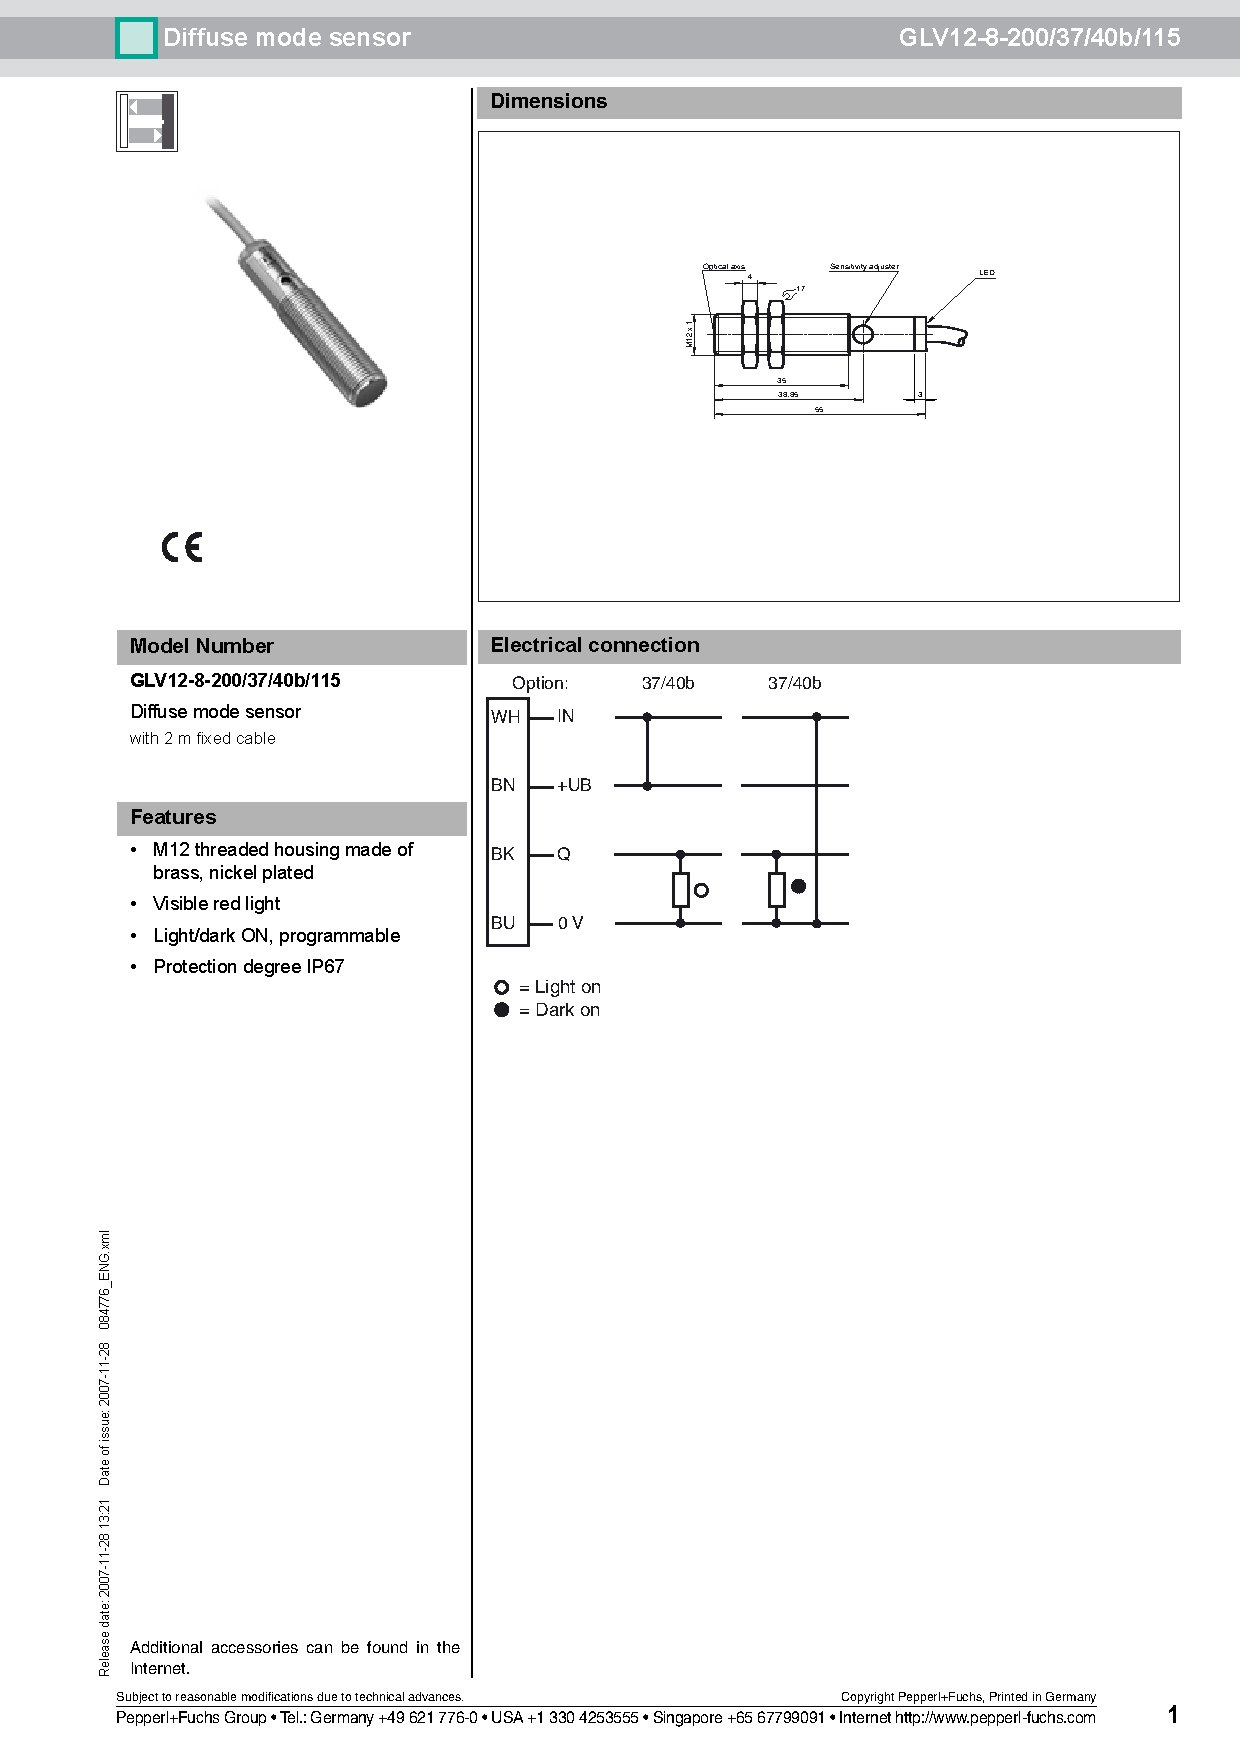
\includepdf[pages=-]{sensorDatasheet.pdf}
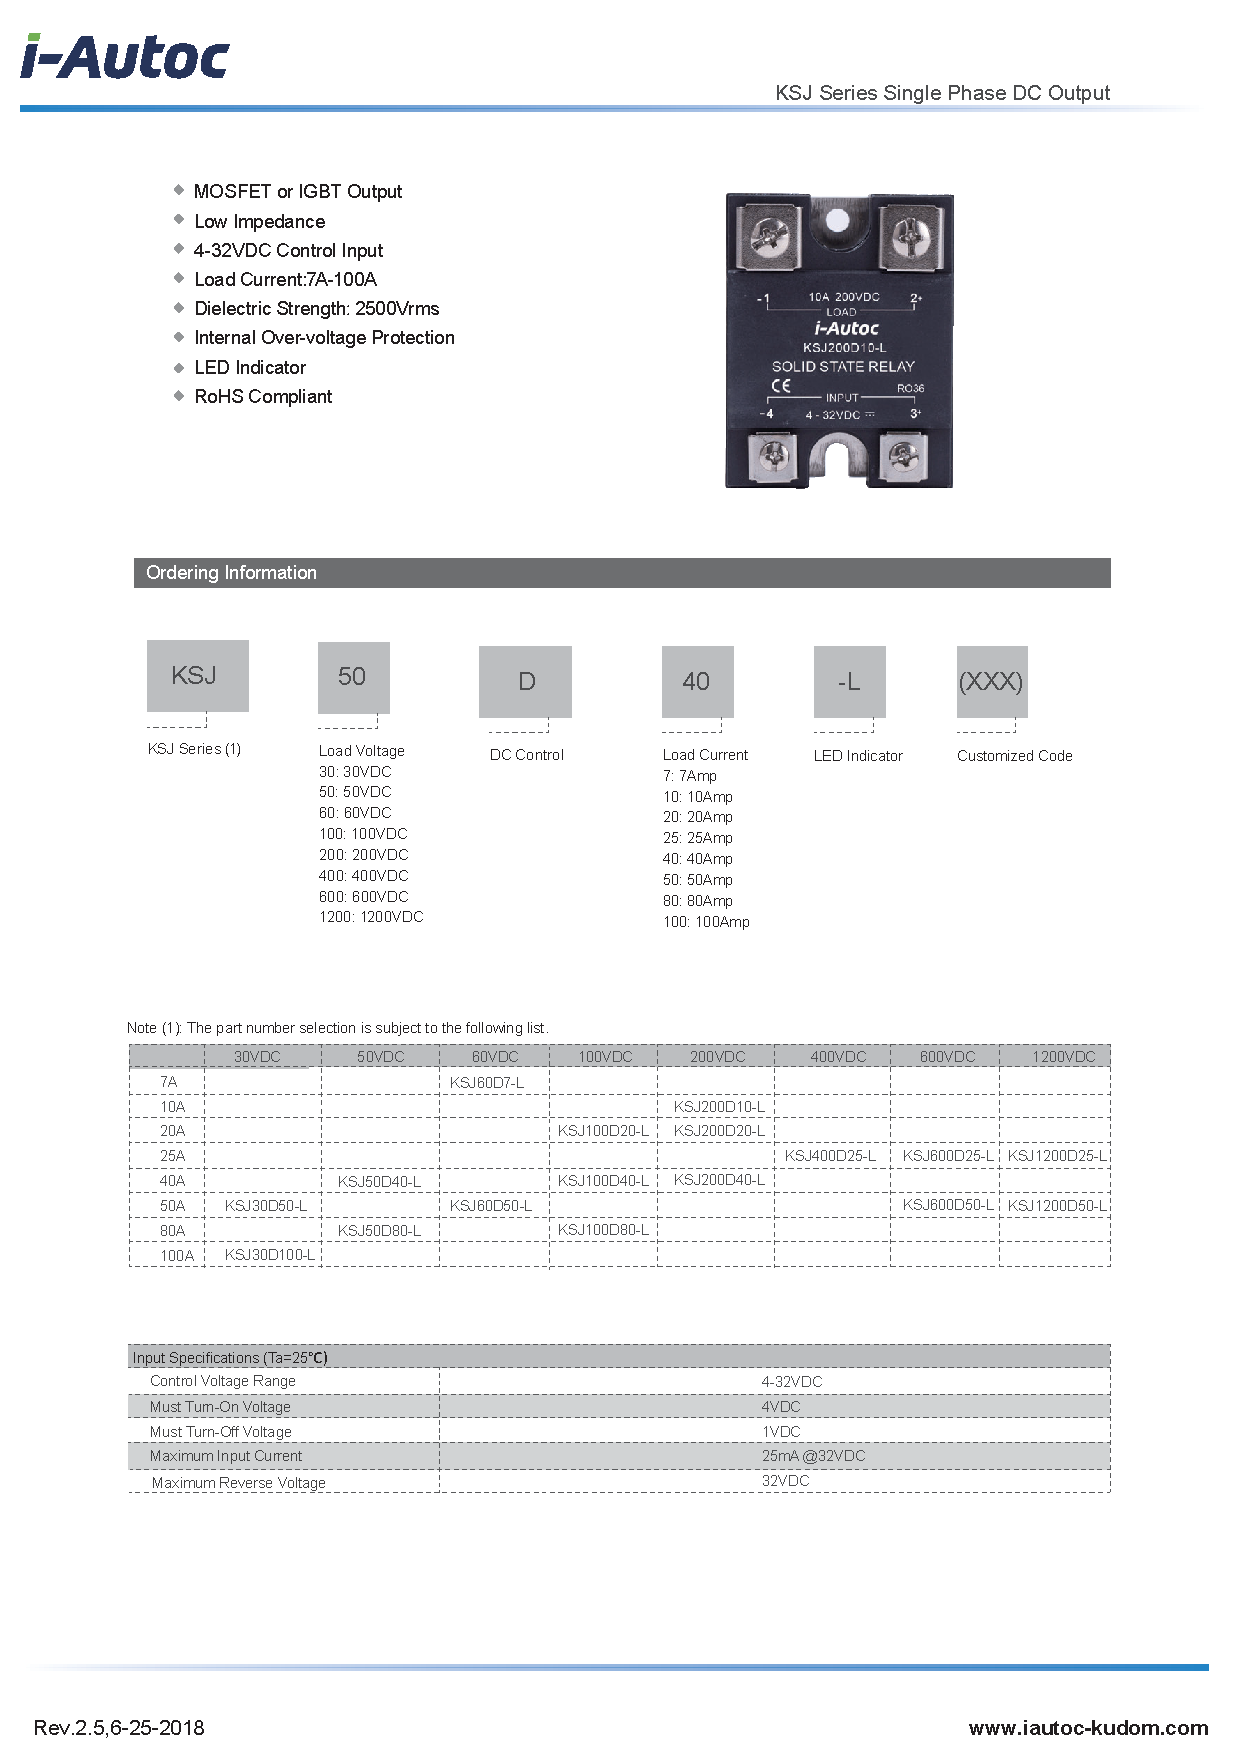
\includepdf[pages=1-5]{ssrDatasheet.pdf}

\end{document}